\documentclass[a4paper, 11pt]{report}
\usepackage[top=2.5cm, bottom=2.5cm, left=2cm, right=2cm]{geometry}
\usepackage{graphicx}
\usepackage{booktabs}
\usepackage{url}
\usepackage[english]{babel}
\usepackage[latin1]{inputenc}
\usepackage{hyperref}
\hypersetup{
    colorlinks,
    citecolor=black,
    filecolor=black,
    linkcolor=black,
    urlcolor=black
}
\usepackage{mathenv}
\usepackage{amsmath}
\usepackage{color}
\usepackage{caption}
\usepackage[bottom]{footmisc}
\usepackage{cancel}
\usepackage{multirow}
\usepackage[toc,page]{appendix}
\usepackage{titlesec}
\usepackage{bm}
\usepackage{mathtools}
\usepackage{subfigure}
\usepackage{cases}

\setlength{\parskip}{1em}
\setlength{\parindent}{0em}
\titleformat{\chapter}[display]
   {\normalfont\huge\bfseries}{\chaptertitlename\ \thechapter}{0pt}{\Huge}

\begin{document}

%Titlepage

\pagenumbering{roman}
\begin{titlepage}

	\centering
	
\includegraphics[width=0.15\textwidth]{figs/image_UC.png} \hspace{20pt} 
\includegraphics[width=0.15\textwidth]{figs/muonSystems.png} \par\vspace{1cm}
	{\scshape\LARGE Facultad de Ciencias \\ Universidad de Cantabria \par}
	
	\vspace{1.5cm}
	
	%English title
	{\huge\bfseries Statistical approach to muography as a non-destructive testing technique for \newline industry problem solving}
	
	\vspace{0.6cm}
		
	%Spanish title
	{\LARGE Muograf\'ia como m\'etodo de prueba estad\'istico y no-destructivo para la resoluci\'on de problemas en la industria \par}
	
	\vspace{2.6cm}
	{\scshape\Large Trabajo de fin de M\'aster \\ para acceder al \par}
	\vspace{0.3cm}
	{\scshape\Large \textbf{M\'ASTER INTERUNIVERSITARIO EN \\ CIENCIA DE DATOS} \par}
	
	\begin{flushright}
	
	\vspace{2.6cm}
	{\Large Autor : C\'edric PRIE\"ELS\par}
	{\Large Director : Pablo MART\'INEZ RU\'IZ DEL \'ARBOL\\}
	{\Large Co-director : CARLOS D\'IEZ\\}
	\vspace{0.5cm}
	{\Large Julio 2020\par}
	\vfill
	
	\end{flushright}

\end{titlepage}

%Empty page

\clearpage
\thispagestyle{empty}
\phantom{a}
\vfill
\newpage

%Abstract and keywords

\setcounter{page}{1}

\section*{\huge{Abstract}}

In this work, cosmic muons have been used to perform a muography experiment, a safe and non-destructive method allowing us to study the internal properties of physical objects with various geometries. Such study is extremely useful in the industry, in order for example to study the degradation of pipes, and finds many application in our daily lives. The main goal of this work was then to find a way to estimate the thickness of steel pipes by studying the deviation undergone by cosmic muons crossing such geometry, using data science and advanced statistical considerations.

In this context, a new C++/ROOT framework has been developed in order to i) recreate the geometry associated to this particular problem, ii) study the results of such muography experiments from a statistical point of view and iii) define a coherent way to estimate the optimal geometrical parameters of different objects placed between two muon detectors using the general properties of muons.

In particular, once defined and fully tested, this framework allowed us to determine the thickness of such steel pipes with a precision of the order of the millimeter.

\begin{center}
\textbf{Key words} : cosmic muons, muography, statistics, geometry, scattering, likelihood
\end{center}

\section*{\huge{Resumen}} 

En este trabajo, muones c\'osmicos se usan para llevar a cabo un experimento de muograf\'ia, un m\'etodo seguro y no-destructivo que permite estudiar las propiedades internas de objetos f\'isicos con diverses geometr\'ias. Estos estudios resultan ser muy \'utiles en la industr\'ia, para por ejemplo estudiar el estado de degradaci\'on de tuber\'ias, y se puede aplicar a muchos temas de nuestras vidas a diario. El objetivo principal de este trabajo consiste en encontrar una manera de estimar el espesor de estas tuber\'ias de acero estudiando la desviaci\'on que sufren estos muones c\'osmicos al atravesar estos objetos, usando cienc\'ia de los datos y m\'etodos estad\'isticos avanzados.

En este contexto, a nuevo framework escrito en C++ y ROOT ha sido desarollado con los objetivos de i) recrear la geometr\'ia asociada a este problema en particular, ii) estudiar los resultados de este experimento de muograf\'ia desde un punto de visto estad\'istico y iii) definir una manera coherente de estimar los par\'ametros geometr\'icos optimos de diferentes objetos puestos entre los dos detectores de muones usando las propiedades generales de los muones.

En particular, una vez definido y comprobado, este framework nos ha permitido detemrinar el espesor de tuber\'ias de acero con una precisi\'on del orden del milimetro. 

\begin{center}
\textbf{Palabras claves} : muones c\'osmicos, muograf\'ia, estad\'istica, geometr\'ia, dispersi\'on, probabilidad
\end{center}

\newpage

%Thank you notes

\section*{\huge{Acknowledgments}}

I would like to mainly thank Pablo for his outstanding work as the director of this project over the past few months. He has been incredibly helpful and present all along the way, teaching me the basic of muography, helping and guiding me when needed. I know it has not always been easy but I am very grateful for the time he spent with me, and I am more than happy with the final result and glad I decided to choose this particular subject.

Thank you to Muon Systems and its CEO Carlos D\'iez in particular, the co-director of this work, for allowing me be a part of their experiment during a few months, granting me a privileged access to actual data simulated and collected. Having the opportunity to work in collaboration with a real industry has been an extremely interesting experience that will for sure help me a lot in the future. I obviously wish to the company all the best for the future since the technology they developed is extremely interesting and definitely shows a lot of potential.

I would also like to thank all the other students involved in this Master degree, in particular Pedro and Nicol\`o, which have both been extremely helpful as well. Many thanks to Lara for organizing this degree in the best way possible given the special circumstances which happened this year and for setting up everything allowing me to follow the classes remotely during the first semester.

Finally, many thanks to my parents and family in general for being there whenever I need it and for supporting my decision to come and study in Spain 6 years ago. It has been a great experience that taught me a lot and that I will for sure never forget.  

%\section*{\huge{Note on my personal work}}

\newpage

%Table of contents

\tableofcontents

\thispagestyle{empty}
\newpage

%Here it starts!
\pagenumbering{arabic}

%Introduction

\chapter{Introduction}

Muon tomography (MT) or simply Muography, is an active field of research nowadays since it provides a non-destructive technique (NDT) allowing to map the inside of large objects where the access is difficult and/or dangerous, without any contact or damage, and without even having physical access to them. To do so, this technique uses cosmic muons, elementary particles similar to electrons but with a much greater mass, which allows them to penetrate much deeper and probe matter in a more efficient way, since they suffer less from the bremsstrahlung radiation affecting all leptons. This technology is relatively well-know and presents several advantages over other similar techniques such as X-ray imaging since it is globally safe, clean by definition (it uses natural radiation) and provides an excellent penetration power in matter.

In this work, MT will be applied to problems related to the heavy industry. In particular, it will be used to probe pipes in the context of the heavy and oil industry, with the target of determining their inner properties and study their degradation. This is the main objective of the company called Muon Systems, founded in 2015 and based in Bilbao.

This company already built powerful muon detectors allowing to perform this task and developed over the years a powerful framework allowing to study the degradation of pipes using convolutional neural networks. However, this method is limited in the sense that training such networks is computing intensive and time consuming, and therefore does not allow to study several properties and geometrical parameters of such pipes at once. In this work, an alternative method based on a statistical analysis of the problem is presented, allowing for a greater generalization of the previous method to other object geometries and to a higher dimension parameters phase space.

This project is highly relevant in today's society because it allows to combine data science algorithms and high-performing statistical methods that have been developed in this context to solve this particular MT problem, putting such methods in practice in an actual industry.


























\chapter{Muons and muography}

The basic physics principles used in the muography technique will be briefly introduced in Section~\ref{sec:particlePhysics} of this Chapter. Muons are particles produced naturally by cosmic rays, themselves introduced in Section~\ref{sec:cosmicRays} and, once produced, they interact when crossing the atmosphere and matter in ways described in Section~\ref{sec:interactions}. These processes need to be understood extremely well for the MT process, introduced in Section~\ref{sec:tomography}, to be useful and applicable to the industry. Finally, the actual experimental setup used for this work will be described in Section~\ref{sec:setup}.

\section{Particle physics and muons} \label{sec:particlePhysics}

Particle physics is the field which studies the matter surrounding us, along with the fundamental interactions between the particles. In this context, the Standard Model of particle physics \cite{SM} is nowadays the most accepted mathematical model used to describe the elementary particles and three of the four fundamental forces of nature (electromagnetic, weak and strong interactions, while the gravitational interaction is out of reach of this model). Even though quite simple in concept, it has been able to describe most of the phenomena observed in nature so far with an incredible level of precision, and has made a lot of predictions that have now been proven to be true, such as the discovery of the top quark \cite{topQuark} in 1995, the tau neutrino \cite{tauNeutrino} in 2001 and the Higgs boson itself \cite{HiggsDiscovery1, HiggsDiscovery2}, the last missing piece of the Standard Model, announced at CERN in July 2012.

According to this model, 12 different fermions (along with their 12 corresponding anti-particles) exist in nature, as shown in Figure~\ref{figure:SMFermions}, most of them being unstable. These fermions can be divided into two fundamentally different categories, the quarks and the leptons, containing each 6 particles and sensitive to different forces. Even though quite interesting, the quarks do not play a fundamental role in the muon tomography detailed in this work, so only leptons will be considered from now on. In particular, leptons can be divided even more into three different generations of particles, and the muon, one particular lepton belonging to the second generation, will be the main focus of this work.

\begin{figure}[htbp]
\begin{center}
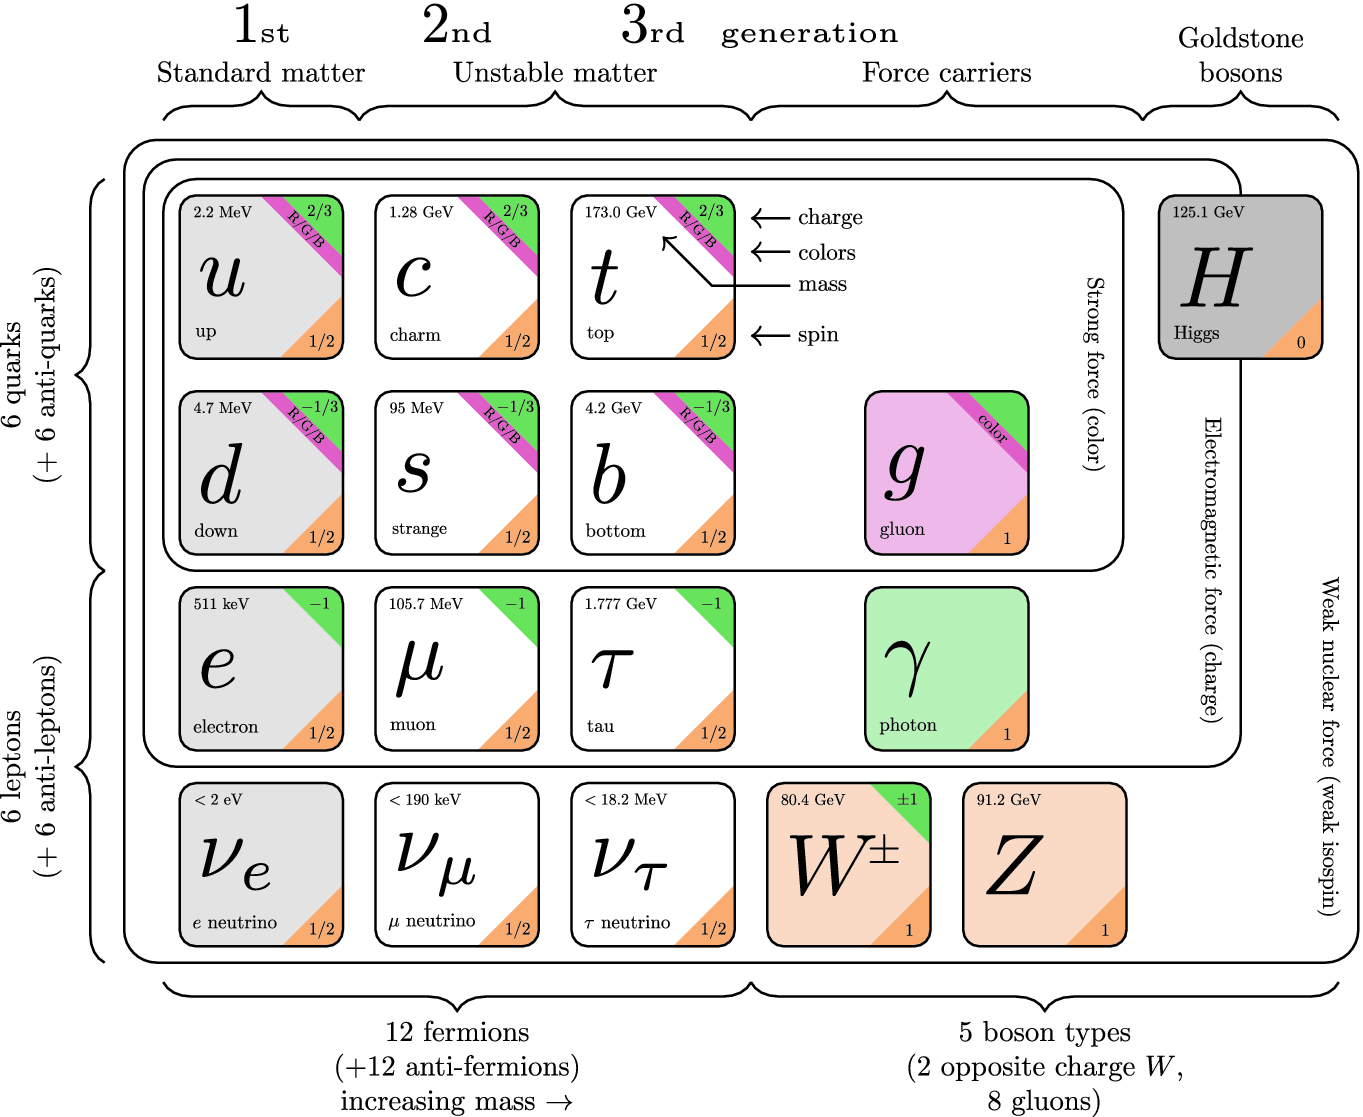
\includegraphics[width=10cm, height=8.2cm]{figs/SMFermions.png}
\caption{Representation of the 12 fermions of the Standard Model \cite{SMFermions} along with the main force carriers and the Higgs boson, discovered in 2012 and completing this model.}
\label{figure:SMFermions}
\end{center}
\end{figure}

Muons $\mu^{-}$ \cite{PDGMuons} are therefore fundamental particles having a negative charge and quite similar in nature to electrons, even though they have a higher mass (200 times larger than the electron), which implies that they are not stable particles: they have a lifetime of approximately 2.2$\mu$s, and typically decay into an electron and a pair of neutrinos. However, this lifetime is actually quite long with respect to other fundamental particles and muons are on average able to travel more than 700 meters, allowing us to consider them to be stable particles in many processes, such as the one presented in this work. Muons also have a relatively small interaction cross-section with ordinary matter, even though they do interact with baryonic matter by several processes described in Section~\ref{sec:interactions}.

\section{Cosmic rays} \label{sec:cosmicRays}

Being unstable by nature, once produced, muons decay almost instantly by a weak process into an electron and a pair of neutrinos. However, it is possible to observe them in nature, since they are continually produced, mainly thanks to cosmic rays \cite{cosmicPDG}, a constant flux of high energy particles (mostly protons and atomic nuclei) coming from many different sources, including supernovae explosions and AGN emissions, and reaching the Earth every day. Indeed, as they impact our atmosphere, these particles start a chain reaction, as shown in Figure~\ref{figure:cosmic}: first of all, several neutral and charged pions are produced, decaying themselves into a pair of photons (and, later on, electron and positron pairs) and muons and neutrinos, respectively.

\begin{figure}[htbp]
\begin{center}
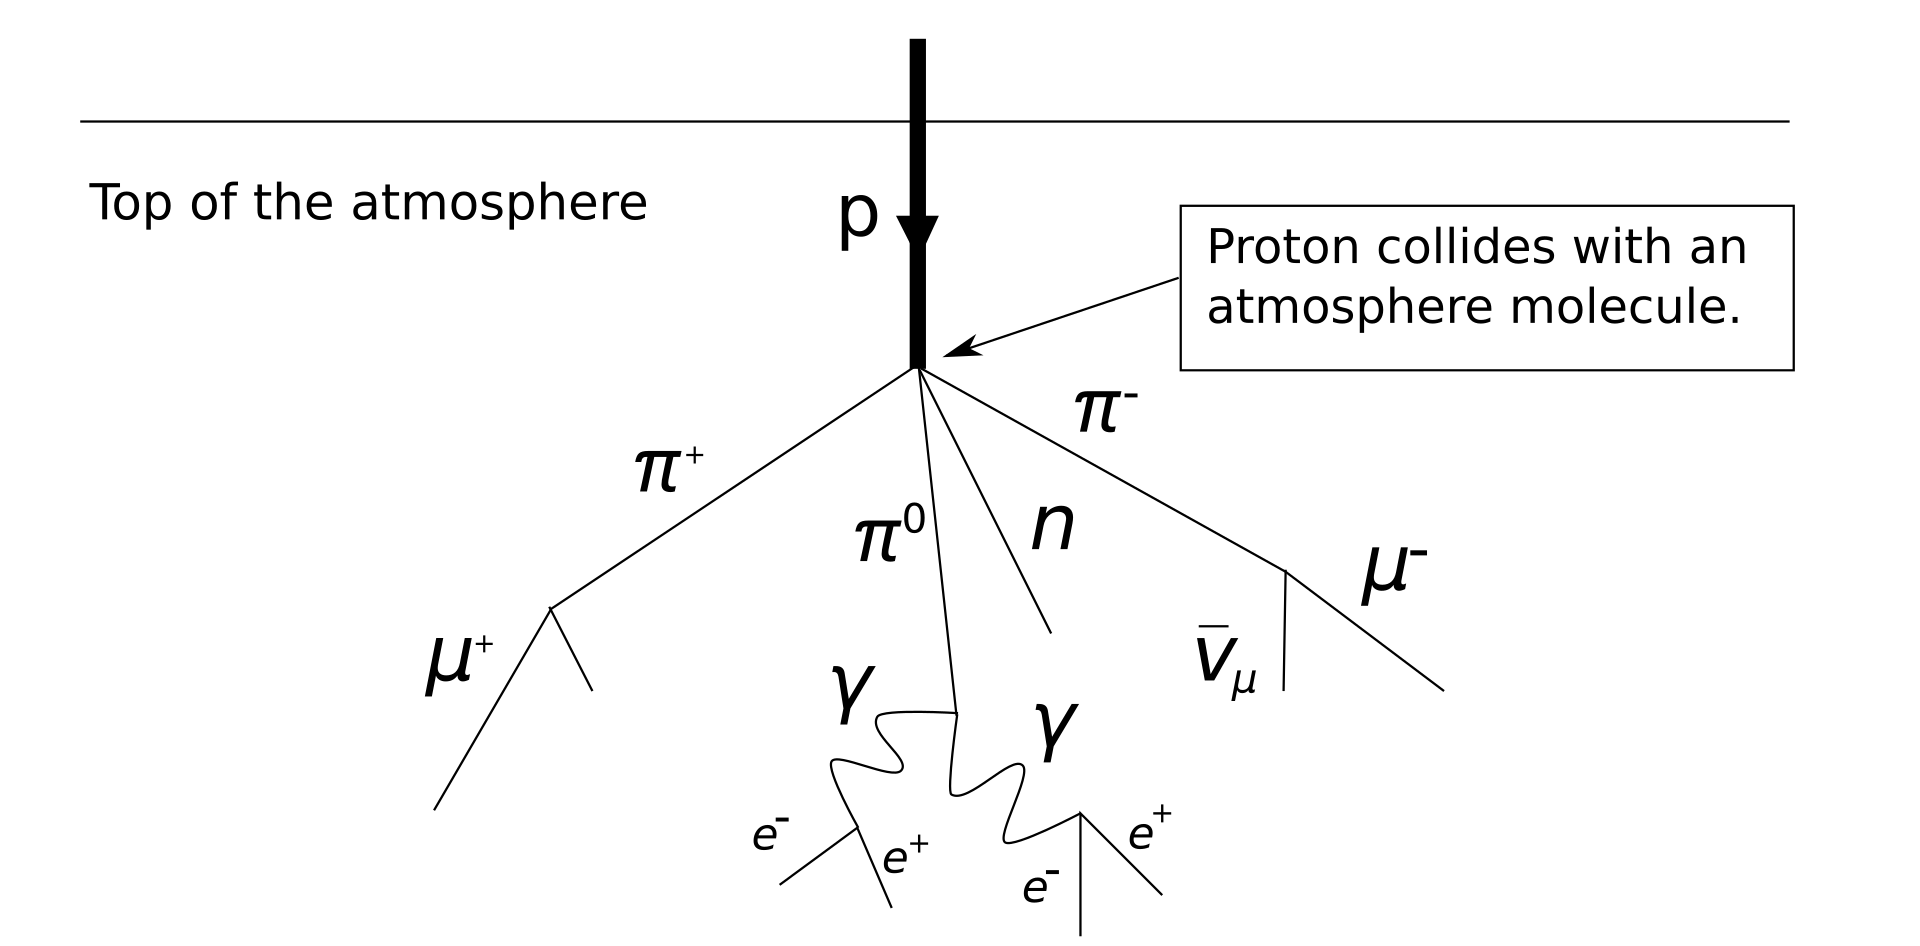
\includegraphics[width=11cm, height=6cm]{figs/cosmic.png}
\caption{Typical chain of decays induced by highly energetic cosmic rays when reaching the Earth's atmosphere and colliding with an atmosphere molecule.}
\label{figure:cosmic}
\end{center}
\end{figure}

\newpage
Muons are the most abundant charged particles produced by these processes actually reaching the sea level, as shown in Figure~\ref{figure:cosmicAbundance}. Even though they are unstable and have a limited lifetime, around 0.06\% of muons produced by such processes do manage to reach the sea level thanks to the time dilation induced by their high energy and relativistic speed. As a rule of thumb, one can expect to observe 10.000 muons per square meter and per minute at the sea level. Muons were actually discovered thanks to cosmic rays in 1936 \cite{muonDiscovery}.

\begin{figure}[htbp]
\begin{center}
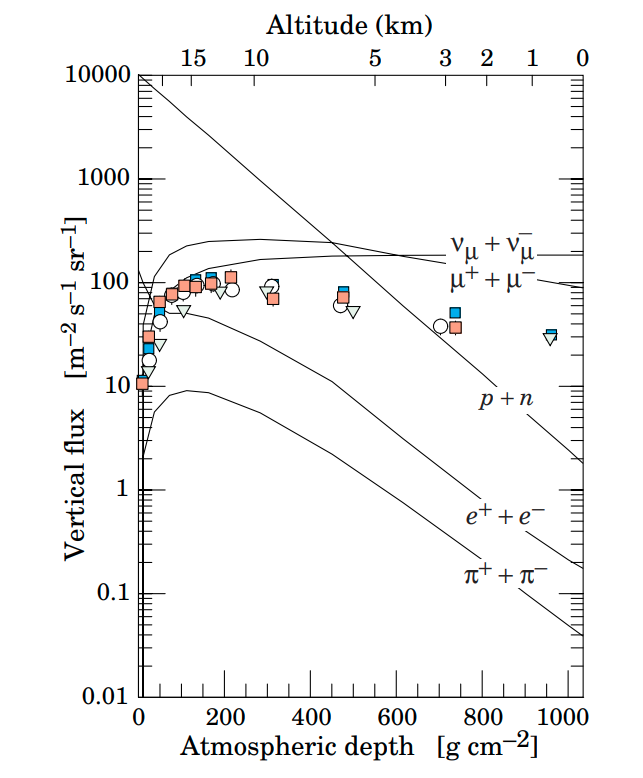
\includegraphics[width=8.5cm, height=9cm]{figs/cosmicMuons.png}
\caption{Abundance of particles due to cosmic rays and observed at the sea level \cite{cosmicPDG}.}
\label{figure:cosmicAbundance}
\end{center}
\end{figure}

The existence of these cosmic rays is critical for this work, since they play the role of the source able to give us the muons we need in order to perform our tomography experiment.

\section{Muons interaction with matter} \label{sec:interactions}

Most of the muons originating from cosmic rays interact with ordinary matter through two main processes: ionization and multiple scattering, both resulting in different effects on the incident particle.

\subsection{Ionization process}

First of all, cosmic muons can interact with matter through \textbf{ionization}, when the incident muon gives some of its energy to the electrons of the absorber. This process is well described by the famous Bethe-Bloch formula shown in Equation~\ref{eq:BB} \cite{PDGMuons}, relating the average loss of energy over a distance $\frac{dE}{dx}$ (typically referred to as the \textbf{mass stopping power}) of material with several parameters, such as the charge number of incident particle $z$ (for cosmic muons, $z = 1$), the atomic mass and charge of absorber $A$ and $Z$, the relativistic factors $\beta$ and $\gamma$, the maximum possible energy transfer to an electron in a single collision $W_{\text{max}}$ and the mean excitation energy $I$.

\begin{equation}
\label{eq:BB}
- \Bigl \langle \frac{dE}{dx} \Bigr \rangle = K z^2 \frac{Z}{A} \frac{1}{\beta^2} \left [\frac{1}{2} \ln \left (\frac{2 m_e c^2 \beta^2 \gamma^2 W_{\text{max}}}{I^2} - \beta^2 - \frac{\delta(\beta \gamma)}{2} \right ) \right ]
\end{equation}

This previous equation gives an accuracy of a few percent in the range $0.1 < \beta = \frac{v}{c} < 1000$ and we can easily see that the quantity of energy lost by a muon when crossing any given medium actually depends on the energy of the incident muon, as shown in Figure~\ref{figure:BB}. In practice, this means that cosmic muons, having a mean energy of a few GeV, have mean energy loss rates actually close to the minimum: they are usually called for this reason \textit{minimum ionizing particles} or MIPs. Energy losses of muons due to this ionization process are for this reason quite small and difficult to detect, so this interaction process will not be considered in this work.

\begin{figure}[htbp]
\begin{center}
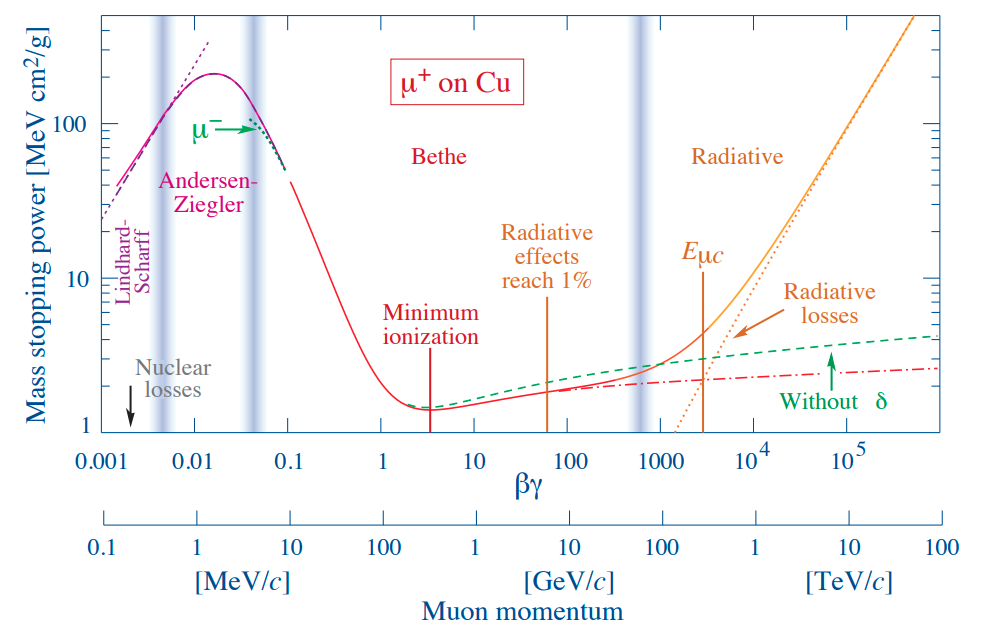
\includegraphics[width=12cm, height=8cm]{figs/BB.png}
\caption{Mass stopping power of copper, or energy lost by a muon in copper due to the ionization process, with respect to its momentum \cite{PDGMuons}.}
\label{figure:BB}
\end{center}
\end{figure}

\subsection{Multiple scattering process}

Muons also interact with matter through another process, called \textbf{multiple scattering}. Since muons have a negative electric charge, by getting close to the nuclei of the absorber, they are suffering from Coulomb scattering. Given the high number of nuclei in matter, this process is repeated many times, deflecting each time the muon by a small angle in a stochastic way, meaning that there is no way of calculating this deviation exactly, but only using probabilities and the so-called theory of Moli\`ere \cite{Moliere}.

According to this theory, the central 98\% of the projected angular distribution due to Coulomb scattering can be described with a Gaussian function, whose width is given by the $\theta_0$ parameter shown in Equation~\ref{eq:Moliere} \cite{PDGScat}, where $p$ is the momentum of the incident particle and $X_0$ is the radiation length, defined as the characteristic amount of matter traversed by the incident particle for a particular interaction. Such dependence on both these parameters has several physical consequences: a muon with a higher momentum (larger $\beta$) will be statistically less deflected, while a muon crossing a medium more dense will be statistically more deflected.

\begin{equation}
\label{eq:Moliere}
\theta_0 = \frac{13.6 \text{ MeV}}{\beta c p} \sqrt{\frac{x}{X_0}} \left [1 + 0.038 \ln \left (\frac{x}{X_0 \beta^2} \right ) \right ]
\end{equation}

This formula, whose second term is actually typically neglected, being much smaller and therefore having a small impact on the final results obtained, is expected to be valid for distances up to $\sim 100 X_0$, giving an error smaller than 11\%. Corrections do exist though in order to get slightly better results, especially in the tails of the distribution, but this theory is precise enough for our needs, given the small deviation angles we expect to observe for the experimental conditions considered.

\begin{figure}[htbp]
\begin{center}
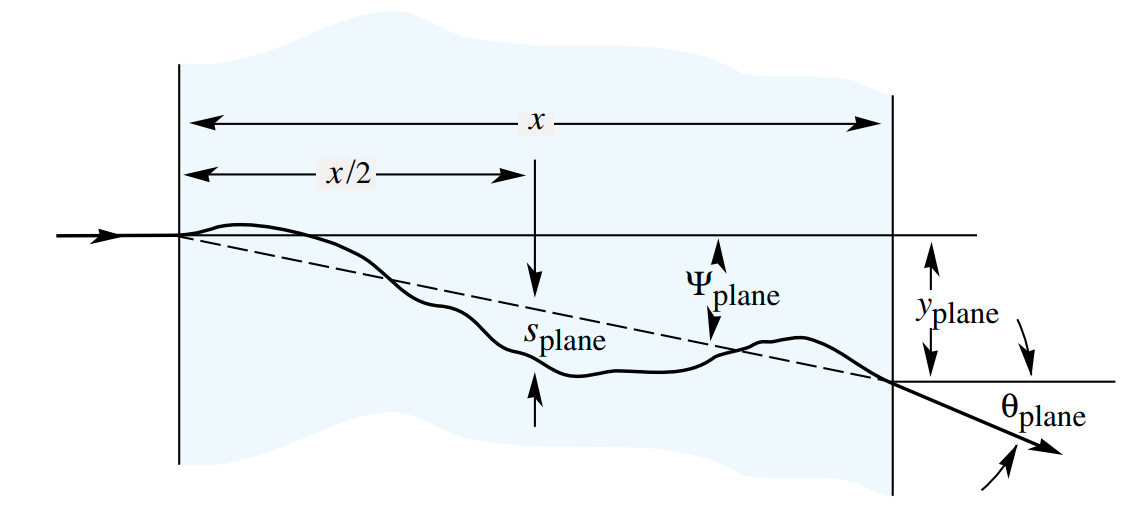
\includegraphics[width=12.5cm, height=5.8cm]{figs/moliere.png}
\caption{Schematic representation of the deviation induced by an absorber to an incident muon because of the multiple scattering effect \cite{PDGScat}.}
\label{figure:Moliere}
\end{center}
\end{figure}

Even though this deviation angle is the most important parameter when considering the multiple scattering, other parameters can be important as well, as shown in Figure~\ref{figure:Moliere}, such as the value of $y_\text{plane}$, shown in Equation~\ref{eq:parameters} corresponding to the deviation observed with respect to the initial expected position. All these additional parameters are typically highly correlated $\left (\text{such as } \rho_{y \theta} = \frac{\sqrt{3}}{2} \simeq 0.87 \right)$ to the deviation angle previously defined but cannot be easily described with this simple theory and not exactly relevant to this work anyway, since the deviation angle will be the main parameters studied with the muon tomography method used.

\begin{equation}
    \label{eq:parameters}
    \begin{dcases}
    \psi_{\text{plane}}^{\text{rms}} = \frac{1}{\sqrt{3}} \theta_0 \\
    y_{\text{plane}}^{\text{rms}} = \frac{1}{\sqrt{3}} x \theta_0 \\
    s_{\text{plane}}^{\text{rms}} = \frac{1}{4 \sqrt{3}} x \theta_0
    \end{dcases}
\end{equation}

\section{Muon tomography} \label{sec:tomography}

Given Moli\`ere's theory, it is obvious to see that, instead of \textit{calculating} the expected deviation of a muon crossing a given material, we can instead try and \textit{measure} it, by inverting the two previous relations. Since this deviation depends on several parameters related to the absorber itself, such as its thickness and radiation length $X_0$, we can then infer such parameters experimentally and determine the properties of the medium crossed by cosmic muons. This is the so-called muon tomography, or \textbf{muography}, taking advantage of the interaction of muons with matter to use it in practice.

Muography is therefore a NDT producing a density map of the inside of an object by measuring a flux of muons. Such method presents many different advantages over other imaging techniques such as X-rays, since it usually uses natural cosmic rays to make the measurements, being therefore completely safe. Additionally, muons interact lightly with matter, meaning that they typically have high penetrating capabilities and can therefore probe even large and/or dense objects. Muography can in this sense be applied to many different fields: it has for example even been used in 1970 in order to try and find hidden cavities of pyramids in Egypt \cite{Egypt} and can also be used to characterize nuclear waste \cite{waste} and is even often used in volcanology, to determine whether a pocket inside of a volcano is empty or full of lava \cite{lava}, among many other practical applications. 

Such imaging techniques can be divided into two categories:
\begin{itemize}
\item \textbf{Absorption muography}. In this case, the observed muon flux in a given direction is compared to what is expected to be seen from cosmic rays, trying to interpret the discrepancies between these two values in order to determine the inner structure of the absorber. Only one detector is needed in this case, therefore reducing the cost and making this technique useful mostly to study large objects, even though the low energy loss rates of relativistic cosmic muons imply that such measurements typically take really long, lasting sometimes up to a few months.
\item \textbf{Scattering muography}. On the other hand, the multiple scattering of muons can be used, by placing one detector on each side of the object being studied to determine the deviation in the direction of the flux of incoming muons. The denser and the thicker the material put in between the detectors is, the larger the observed deviation will be, as shown in Equation~\ref{eq:Moliere}. This technique is mostly used to study smaller objects and is able to make quick measurements.
\end{itemize}

In this particular work, scattering muography is being applied to industry in order to try and determine the degradation of the interior of industrial equipment such as steel pipes, as we will now see, starting by a description of the experimental setup that was used with this objective in mind.

\section{Experimental setup} \label{sec:setup}

\subsection{Muon detectors} \label{sec:muonDetectors}

If we want to work with cosmic muons, we need to be able to build devices able to detect them and measure their properties such as their energy and/or direction of propagation. Many different technologies exist nowadays in order to detect muons but in this particular case, the typical \textbf{multi-wire proportional chambers} have been used.

Invented at CERN in 1968, these detectors use an array of high-voltage wires (playing the role of the anode), running through a chamber filled with gas and whose walls are typically grounded (the cathode), as shown in Figure~\ref{fig:wireChambers}. Such an experimental setup therefore creates an electric field inside of the chamber, that needs to be tweaked to be as large and uniform as possible.

\begin{figure}[htbp]
\begin{center}
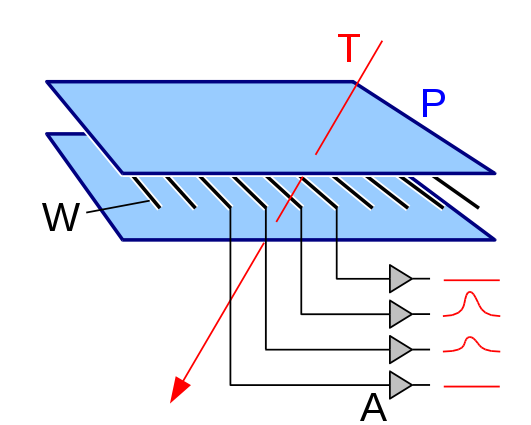
\includegraphics[width=7.2cm, height=5.5cm]{figs/wireChambers.png}
\caption{Schematic representation of a wire chamber muon detector.}
\label{fig:wireChambers}
\end{center}
\end{figure}

When a charged particle such as a muon crosses this chamber, it will ionize the gas of the chamber and leave small electric charges along its path which will start to drift until reaching one of the wire. This drift induces an electric signal proportional to the ionisation effect in the different wires surrounding the particle path, and the combination of all the signals collected by the different wires is able to give information regarding the actual path followed by the incoming particle.	

Several properties are extremely important when designing a detector:
\begin{itemize}
\item First of all, the \textbf{spatial resolution}, the precision by which we can tell the position of the muon, should be ideally as small as possible, depending on the actual problem faced. This can typically be achieved simply by increasing the number of wires in the muon chamber.
\item We also typically want the detector to be large enough to avoid any \textbf{acceptance} issues.
\item Finally, the \textbf{efficiency} is also an important parameter, since we want to be able to detect as many muons as possible, to make the measurement faster and more precise.
\end{itemize}

\subsection{Working setup} \label{sec:ourSetup}

For this particular work, four muon chambers of 1 meter by 1 meter have been build using these principles, as shown in Figure~\ref{fig:setup}. As we can see, more than 200 wires connected to the high voltage and made out of gold and tungsten have been placed every 4 mm in two different planes rotated by 90 degrees, to measure the $x$ and $y$ position of cosmic muons. 

These chambers, filled while a mixture of Argon and CO$_2$, are then setup in pairs above and below the object being studied, in order to determine the position and the direction of the incoming and outgoing cosmic muon. This setup allows to measure with a good spatial resolution the deviation of muons, to determine as precisely as possible the properties of the object put in between both detectors.

\begin{figure}[htbp]
\centering
\begin{minipage}[b]{.59\textwidth}
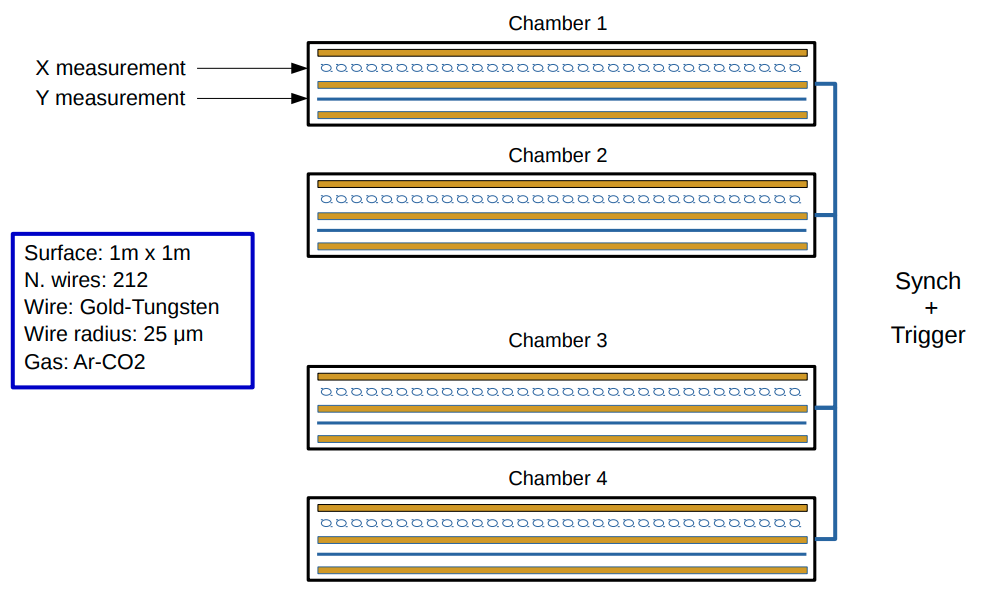
\includegraphics[width=9cm, height=6cm]{figs/muonChambers.png}
\end{minipage}\hfill
\begin{minipage}[b]{.39\textwidth}
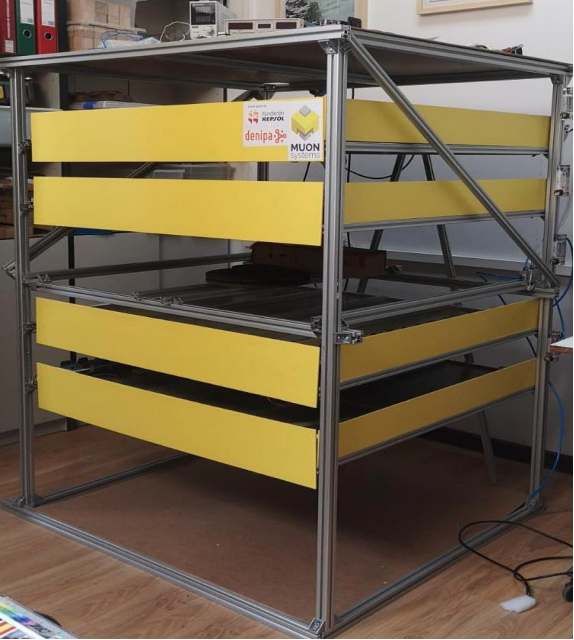
\includegraphics[width=6cm, height=6cm]{figs/muonChambersPhoto.png}
\end{minipage} \hfill
\caption{Actual working setup used for this work, with two multi-wires muon chambers of 1m$^2$ placed on each side of the object being studied.}
\label{fig:setup}
\end{figure}

\subsection{Data flow} \label{sec:dataFlow}

Once collected, the data needs to be passed through several different layers in order to convert electric signals into files that can be processed, as shown on Figure~\ref{fig:dataFlow}. As we can see, the data follows a different path depending on its nature, if it has been collected by the detector or if we are considering Monte-Carlo simulations that will be described in details in the next Chapter. 

The stream of data on one hand is collected by a simple USB, and then sent to a DAQ/DQM system and to an unpacker, which takes into account the detector geometry and translates into a physical position the information received from the DAQ, typically only telling that a certain wire has been activated. On the other hand, the stream for Monte-Carlo, which will be mostly used in this work, relies first of all on CRY \cite{CRY}, a cosmic ray generator able to simulate reliably the incident cosmic muons, and then on Geant4 \cite{Geant4}, a toolkit developed by CERN in order to simulate the passage of particles through matter and through the detectors, by including at this point as well a calibration step related to the expected detector response.

Both streams then join at the 1D histogram format level, gathering a collection of all the hits measured for every event. All these hits are then processed and reconstructed into two trajectories, one above and one below the object, using advanced techniques that will also be described in next Chapter. Finally, 4D segments are made available from this reconstruction process, containing all the position and direction information needed, from which the actual analysis can take place.

\begin{figure}[htbp]
\begin{center}
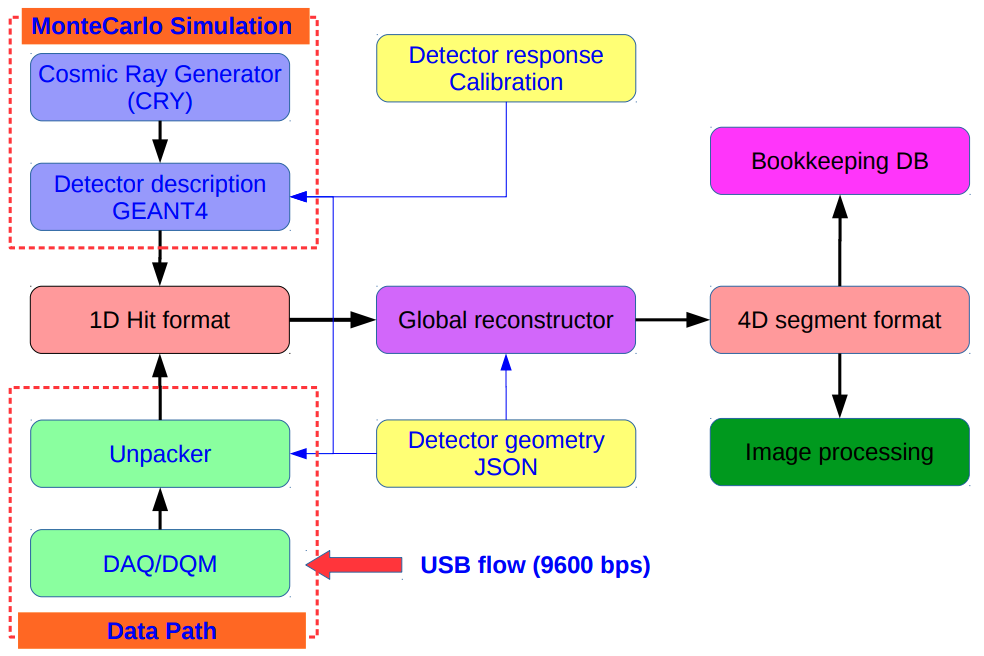
\includegraphics[width=9cm, height=7cm]{figs/dataFlow.png}
\caption{Schematic representation of the detector data flow.}
\label{fig:dataFlow}
\end{center}
\end{figure}



























\chapter{Statistical basis of the algorithm}

The main goal of this work is to find a way to estimate the geometrical parameters of a physical object using a MT technique (in particular, we will focus on the estimation of the thickness of a steel pipe for simplicity). To reach this goal, an algorithm based on a Maximum Likelihood Estimation method  in which the inner radius of the pipe is the parameter and described in Chapter~\ref{chapter:algorithm} has been developed, in order to estimate the interaction between the cosmic muons and the object under investigation to determine its inner properties.

By nature, this algorithm heavily relies on several important statistical concepts that therefore needs to be described first. In this context, concepts such as the probability and kernel density functions (described in Sections~\ref{sec:PDF} and~\ref{sec:KDF} respectively), Monte-Carlo simulations (in Section~\ref{sec:MC}), the probability values (in Section~\ref{sec:pValues}) and the likelihood function (in Section~\ref{sec:Likelihood}) will now be described.

\section{Probability density functions} \label{sec:PDF}

The probability density functions, or PDF, are mathematical expressions defining probability distributions which represent the likelihood of any given outcome. Depending on the problem considered, they are typically represented as curves as shown in Figure~\ref{fig:PDF}, in which the total area below the curve in an interval can be interpreted as the value of the probability of a random variable occurring. 

\begin{figure}[htbp]
\begin{center}
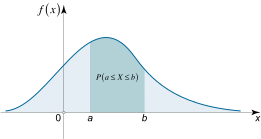
\includegraphics[width=12cm, height=5.4cm]{figs/PDF.png}
\caption{Schematic representation of a random PDF \cite{PDF}.}
\label{fig:PDF}
\end{center}
\end{figure}

The famous Gaussian distributions are in this sense probability density functions which have a particular expression shown in Equation~\ref{eq:gauss}, where $\sigma$ is the so-called \textbf{standard deviation} of the distribution, representing its width: a low $\sigma$ indicates that the values of the distribution tend to be close to its mean value $\mu$, while a high $\sigma$ indicates that the values are spread out over a wider range.

\begin{equation}
\label{eq:gauss}
f(x) = \frac{1}{\sqrt{2 \pi} \sigma} e^{-\frac{1}{2} \left (\frac{x - \mu}{\sigma} \right )^2}
\end{equation}

These definitions are important because we already know that the multiple scattering process which affects the incident cosmic muons is a stochastic process: this means that two muons having similar incident kinematics can leave the detector with very different output positions and directions, whose actual distribution can be approximated by a Gaussian function for small enough deviation angles (at larger angles, the distribution is behaving like Rutherford scattering, with slightly larger tails), according to the multiple scattering theory. 

The probability density function is an important concept in this work since the multiple scattering process of muons is given by a bi-dimensional Gaussian distribution whose covariance depends on the geometrical parameters of the eventual object put between the two detectors, as shown in Figure~\ref{fig:deviation}. This means that, in first approximation, the thicker and denser the object investigated is, the higher the expected deviation will be and this simple observation will actually be used as the driving process of the statistical study performed in this work.

\begin{figure}[htbp]
\centering
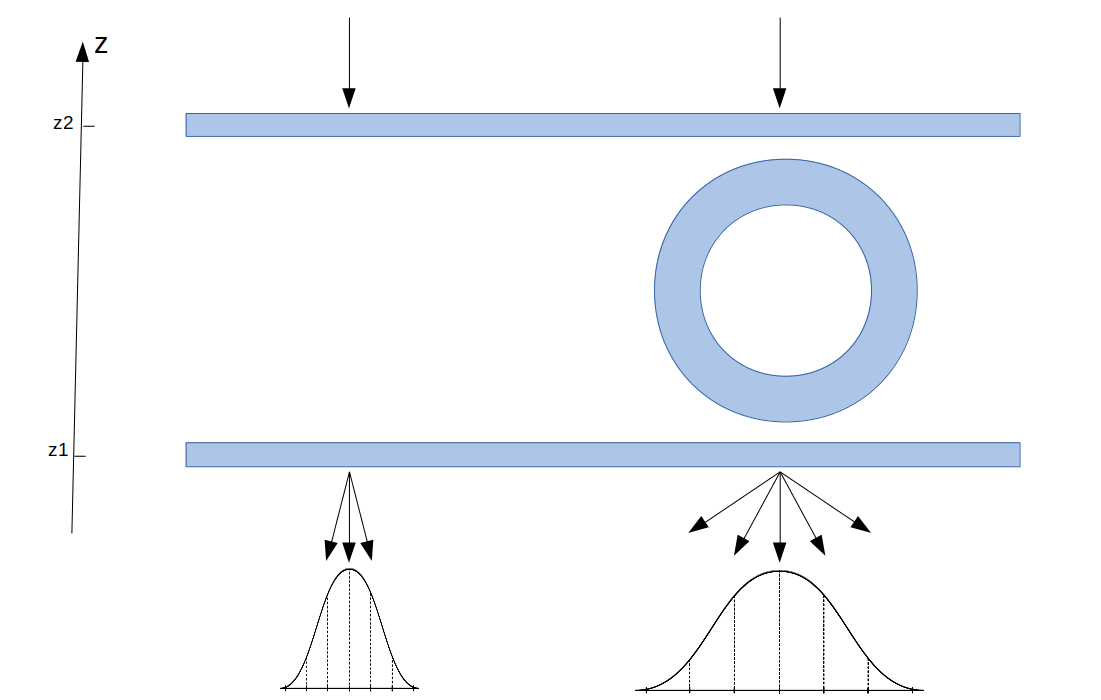
\includegraphics[width=11.5cm, height=7cm]{figs/pdfs.png}
\caption{Schematic representation of the deviation expected for an incoming muon and PDF associated without (on the left) and with (on the right) an object placed between the detectors.}
\label{fig:deviation}
\end{figure}

\section{Kernel density estimations} \label{sec:KDF}

In statistics, the kernel density estimation is a method allowing to estimate the shape of the density probability $f$, the PDF defined in Section~\ref{sec:PDF}, of a random variable $\bm x$, from $N$ observations drawn from this unknown function PDF. The usual way to proceed is to place each observation made in an histogram, where the density in each point $x$ can be therefore be estimated as the proportion of observations close enough to $x$. However, this method depends strongly on the binning used and the function obtained by this process is non-continuous by definition. The \textbf{kernel method} has been developed in this context, to try and solve the non-continuity of the PDF obtained, by simply using various continuous functions instead of bins. This process allows to create a smooth curve given a set of data, which will be something of great interest in this work.

Mathematically, we can define a function called the \textbf{density estimator} of $f$, $\hat{f}_h(x)$, defined as the sum of general functions $K$ over the number of observations drawn, as shown in Equation~\ref{eq:KDF}.

\begin{equation}
\label{eq:KDF}
\hat{f}_h(x) = \frac{1}{Nh} \sum_{i=1}^{N} K \left (\frac{x-x_i}{h} \right )
\end{equation}

In this last equation, two parameters that need to be defined by hand before using this method are actually extremely important:
\begin{itemize}
\item First, the \textbf{kernel} $K$, is a non-negative window function defined depending on the problem, as the "building block" of the final function that needs to be estimated: indeed, as we can see, the function $\hat{f}_h(x)$ will be given as a simple sum of these kernels. In most of the problems, including this work, a standard Gaussian kernel is used, taking the shape shown in Equation~\ref{eq:kernel}.

\begin{equation}
\label{eq:kernel}
K(x) = \frac{1}{\sqrt{2 \pi}} e^{-\frac{1}{2} x^2}
\end{equation}

\item The so-called \textbf{bandwidth} or \textbf{smoothing parameter} $h$ is another interesting parameter, affecting mainly the final smoothness of the resulting curve obtained. The optimal selection of such parameter is not obvious at all \cite{bandwidth} but, as a rule of thumb, it can be shown that for Gaussian kernels of standard deviation $\sigma$, it should be approximately equal to $1.06$ $\sigma N^{-1/5}$ in order to minimize the mean integrated square error obtained. 
\end{itemize}

A comparison of the different methods so far and different possible is shown in Figure~\ref{fig:KGR}.

\begin{figure}[htbp]
\centering
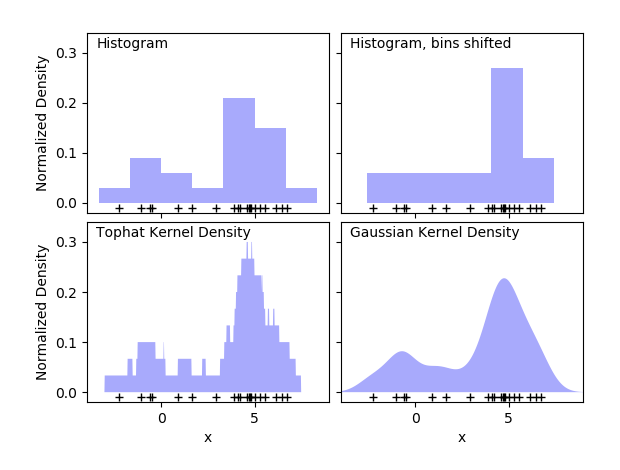
\includegraphics[width=13cm, height=10cm]{figs/kernels.png}
\caption{Comparison of the histogram and the kernel density estimations methods for different kernels in order to estimate a PDF \cite{scikit}.}
\label{fig:KGR}
\end{figure}

In summary, this method is used in order to model the distribution of an arbitrary input dataset as a superposition of Gaussian kernels, one for each data point, each contributing 1/N to the total integral of the PDF. This method allows us to construct continuous functions and recover for the eventual low statistics and possible gaps in the bi-dimensional histograms for the position and direction of the muons obtained in $x$ and $y$, following the method that will be described in Chapter~\ref{chapter:algorithm}.

\section{Monte-Carlo simulations} \label{sec:MC}

Monte-Carlo simulations are generated from algorithms developed in order to compute approximate numerical values to stochastic problems using random processes and advanced probabilistic techniques. In this particular case, such computation methods apply extremely well since, by being a stochastic process, the actual probability density function associated to a given geometry cannot be computed analytically (and if we were able to do it, a simple gradient descent method would be enough to solve this problem and find the optimal parameters \{$\theta_i$\} of the object). 

The only way available to actually estimate these parameters is by using thousands of Monte-Carlo simulated toys, simulating thousands of different incident muons for different geometries. The principle is simple: for each incident muon measured, a large number $N_{\text{MC}}$ of Monte-Carlo simulations will be performed, propagating the muon using an algorithm described in Chapter~\ref{chapter:algorithm} until reaching the lower detector. Repeating this experiment over and over again always gives different results, giving us the opportunity to build the expected PDF for a given object geometry and for the incident muon that has been measured and that will be used later on.

At the end of the day, the main objective of this process is to be able to estimate the probability of observing a certain deviation given an object geometry and the input trajectory of the muon, $P$(deviation$|$input) in simulation. Once done, this process can then be reversed using actual data in order to try and obtain the geometry of the object from the actual measurement of the input and output muon trajectories and positions, using a likelihood minimization method.

\section{Probability values} \label{sec:pValues}

So far, we developed a technique allowing us to reconstruct the expected probability density function for a given incident muon using Monte-Carlo techniques. However, we still need a way to estimate the goodness of the actual measurement with respect to this simulated PDF. This is where the so-called \textbf{p-values} enter, a key ingredient for this work since they allow to relate the two main parts of the problem: the simulations performed and the actual data collected.

Probability values, or p-values, are based on the concept of the \textbf{null hypothesis $H_0$}, a general statement or default position telling that there is no actual relationship between two measured phenomena and assumed to be true until an evidence indicates otherwise. This hypothesis is then typically opposed to the \textbf{alternative hypothesis $H$}, usually more interesting by being the interesting hypothesis of the experiment being performed. The main goal is to compare the data with both hypotheses: if the data is consistent with $H_0$, then the null hypothesis can simply not be rejected. However, we can reject $H_0$ (and therefore accept $H$, its exact opposite) if the data collected is significantly unlikely to have occurred if the null hypothesis were to be true, according to a certain \textbf{confidence level}.

From these definitions, a p-value is then defined as the probability for a variable to be observed equal or more extreme (lower or higher, depending on the problem) than the actual value $x$ observed under the null hypothesis. This definition, can be represented in a schematic way in Figure~\ref{fig:pvalue}.

\begin{figure}[htbp]
\centering
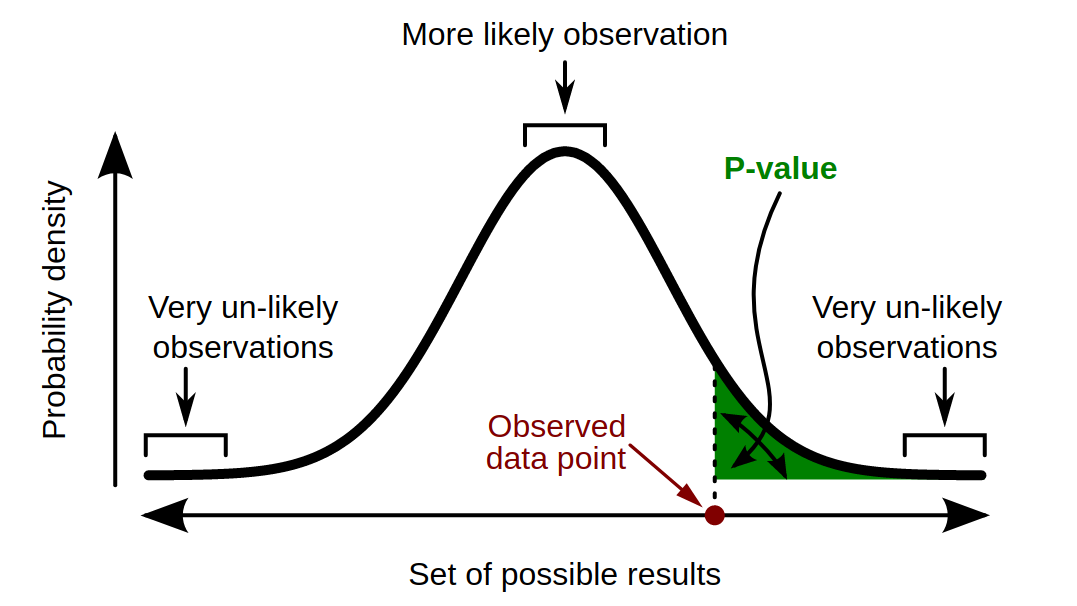
\includegraphics[width=13cm, height=7cm]{figs/pvalue.png}
\caption{Schematic representation of the statistical concept of p-value.}
\label{fig:pvalue}
\end{figure}

In general, a smaller p-value indicates us that the hypothesis $H$ under consideration may not adequately explain the observation. At the end of the day, the null hypothesis can be rejected only if the p-value obtained is smaller than a previously defined, arbitrary and fixed threshold $\alpha$, the so-called \textbf{level of significance} of the experiment. This parameter can take a large range of values, typically ranging from 0.05 to 0.001.

Even though this is an extremely important parameter that could be used, in this particular work however, we don't really to go through this whole need to estimate the PDF integral from a certain value, we only need to estimate the value of the PDF at a given position. This value will then be fed to a likelihood function, as explained in Section~\ref{sec:Likelihood}.

\section{Likelihood} \label{sec:Likelihood}

So far, we have been able to generate thousands of different Monte-Carlo experiments for a given muon and for a given object geometry, but we still need to find a way to reverse this process to estimate the geometry of the object from a given measurement. 

This is where the likelihood becomes useful, defined as a function that measures the goodness of a fit with respect to a sample of data, for several unknown parameters of a mathematical model. In general, this function can be defined in Equation~\ref{eq:likelihood}, where $\bm \theta = $\{$\theta_1, ..., \theta_i$\} are the parameters of the model and $x$ is the actual measurement of a random variable $X$ following a density function $f$.

\begin{equation}
\label{eq:likelihood}
\mathcal{L}(\bm \theta | x) = f_{\bm \theta}(x) = P(X = x | \bm \theta)
\end{equation}

It is important to note at this point that the likelihood is a function of the parameters $\bm \theta$ but not a probability density function itself. Additionally, it should in general not be confused with the probability $p(\bm \theta | x)$ since it is equal to the probability of observing a given outcome $x$ when the true values of the parameters are $\bm \theta$: this means that the likelihood is equal to a probability density over the outcome $x$, not over the set of parameters $\bm \theta$.

To understand this concept better, the simple example of an unfair coin toss can be considered, where the fairness of the coin is the parameter of the model, represented by the probability of obtaining head $p_H$ and taking values between 0 and 1 (for a regular coin, $p_H = 0.5$). The likelihood is then defined from a given observation, such as obtaining two heads in a row $HHT$ in the following way:

\begin{equation}
\label{eq:likelihoodEx}
\mathcal{L}(p_H | HHT) = P(HHT | p_H) = P(H | p_H) \cdot P(H | p_H) \cdot P(T | (1-p_H))
\end{equation}

For each value of $p_H$, the value of the likelihood can then be computed and ultimately plotted, as shown in Figure~\ref{fig:likelihoodEx}, showing a minimum value for a particular value of $p_H$. Often, the \textbf{log-likelihood} $l(\bm \theta | x) = -2 \log(\mathcal{L}(\bm \theta | x))$ is actually used instead, being a bit more convenient to deal with the special part concavity plays in the maximization process. Given the properties of the logarithm, maximizing the likelihood is equivalent to minimizing this particular log-likelihood

\begin{figure}[htbp]
\centering
\begin{minipage}[b]{.49\textwidth}
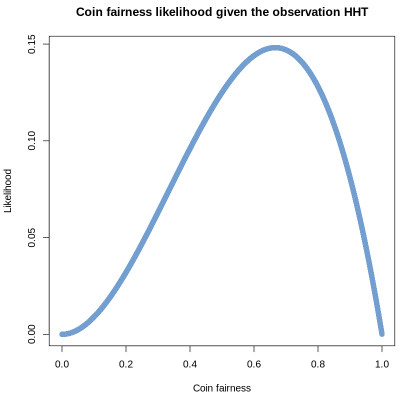
\includegraphics[width=7.8cm, height=6.8cm]{figs/likelihood.png}
\end{minipage}\hfill
\begin{minipage}[b]{.49\textwidth}
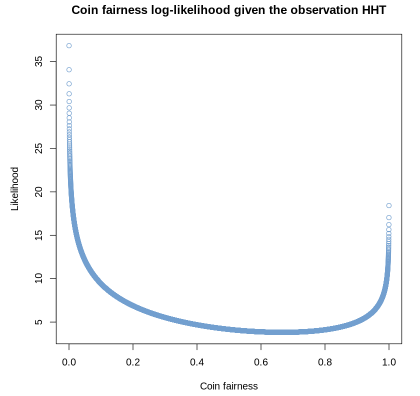
\includegraphics[width=7.8cm, height=6.8cm]{figs/loglikelihood.png}
\end{minipage} \hfill
\caption{Likelihood (on the left) and log-likelihood (on the right) obtained for our particular example of the fairness of a coin given the observation $HHT$.}
\label{fig:likelihoodEx}
\end{figure}

The likelihood is in this sense interesting because it can be described as an hypersurface whose peak gives the optimal set of parameters maximizing the probability of drawing the actual sample measured. Another important property of the likelihood that will be used extensively and already assumed in the previous example is the fact that, for two independent measurements, the likelihood of both measurements is equal to the product of both likelihoods independently computed for each event.

In this work, the objective is to estimate how likely it is that we observed a given set of measurements for a particular pipe geometry. This is done by computing the PDF of the positional and angular deviation of cosmic muons from Monte-Carlo simulations and by then evaluating the actual PDF value for a given measurement along both the $x$ and $y$ axes, the total likelihood being defined as the product of such values obtained for the thousands of muons collected for a given geometry. A general maximum likelihood estimation method is then used, which consists in finding the best possible estimator, referred to as $\bm \hat \theta$, by minimizing the log-likelihood obtained by considering several different object geometries put between the detectors, allowing us to find the optimal set of parameters (such as the thickness of the pipe) able to describe in the best way possible this object. Indeed, from the definition of the likelihood in Equation~\ref{eq:likelihood}, we can see that the $\bm \hat \theta$ which maximizes the likelihood will also maximize the probability of observing the data measured for a given geometry.










%In this work, measurements of cosmic muons are taken for a relatively long period of time to accumulate statistics. Each event recorded is independent from the previous one by nature, and our goal is to estimate from the ingredients previously defined the actual geometry of the object placed between the detectors, defined from a set of parameters $\bm \theta$.

















\addtocontents{toc}{\protect\newpage}
\chapter{The algorithm} \label{chapter:algorithm}

The algorithm we developed to solve this particular problem has been written in C++ and can be divided in three categories. First of all, we have the so-called \textbf{PipeReconstructor} (Section~\ref{sec:PipeReconstructor}), a set of classes able to perform several tasks:
\begin{itemize}
\item Define the geometry of the problem (the detector, and the volume under investigation are therefore defined using the smallest possible set of parameters at this stage);
\item Compute the different intersection points of an incident cosmic muons with our geometry;
\item Propagate the muons through the different medium of interaction encountered along their path using the Moli\`ere's theory of multiple scattering;
\item Calculate the likelihood of a given measurement for a given volume;
\item Finally, probe different volumes and perform a descent method in order to minimize the likelihood encountered and find the optimal volume to solve our problem given the measurements collected. 
\end{itemize}

This class is complemented with the \textbf{Generator} (Section~\ref{sec:Generator}), a small class allowing us to generate muons simulating our actual experiment, using some of the functions of the PipeReconstructor. Usually, the Monte-Carlo simulation and event reconstruction is performed using the Geant4 toolkit, a reliable method able to describe precisely the interaction between the detector and the incident muons. However, this process is quite slow and in this work, we then developed this Generator as an alternative faster reconstruction method that will be thoroughly validated in Chapter~\ref{chapter:results}.

Finally, a \textbf{Plotter} (Section~\ref{sec:Plotter}) comes in play, allowing us to plot the different interesting variables such as the likelihood curves for different geometries, a crucial step of the minimization process.

\section{PipeReconstructor} \label{sec:PipeReconstructor}

The PipeReconstructor is a set of classes allowing us to define different kind of physical and statistical objects essential to solve the original problem.

\subsection{MuonState}

First of all, a muon is defined from the \textbf{MuonState} class and from 7 parameters: 3 parameters ($x$, $y$, $z$) representing the position of the muon, 3 additional parameters ($v_x$, $v_y$, $v_z$) representing its three-dimensional direction, and the actual value of its momentum. The measurement performed at the top detector will be labelled with the index 1 ($x_1$, $y_1$, $z_1$, $v_{x1}$, $v_{y1}$, $v_{z1}$, $p_1$) while the measurement performed by the lower detector will take the index 2.

\subsection{Surfaces and volumes}

\textbf{Surfaces} and \textbf{Volumes} are virtual classes allowing us to define general surfaces (their spatial position and their geometrical center) and volumes, defined as vectors of several surfaces: a general volume is in this sense defined by its surfaces, central position and global density. Defining such virtual classes is extremely important since it would allow us to consider different geometries, not just a pipe put in between the two detectors. The constant size ($1 m^2$) and $z$ position of both the lower and upper detectors (-37 and 37 cm, respectively) are also defined as constants at this stage.

\subsection{Cylinders and pipes}

\textbf{Cylinders} and \textbf{Pipes} are particular subclasses of the virtual classes previously defined in order to define the geometry of this particular problem. A pipe is in this sense defined as a set of two cylinders and from 7 different parameters: its central position ($x$, $y$, $z$), along with its density, the radii $r$ and $R$ of both cylinders and its length along the y-axis $L$, as shown in Figure~\ref{fig:cylinder}. For simplicity, the pipes considered in this work are therefore considered to have a constant density.

\begin{figure}[htbp]
\centering
\begin{minipage}[b]{.49\textwidth}
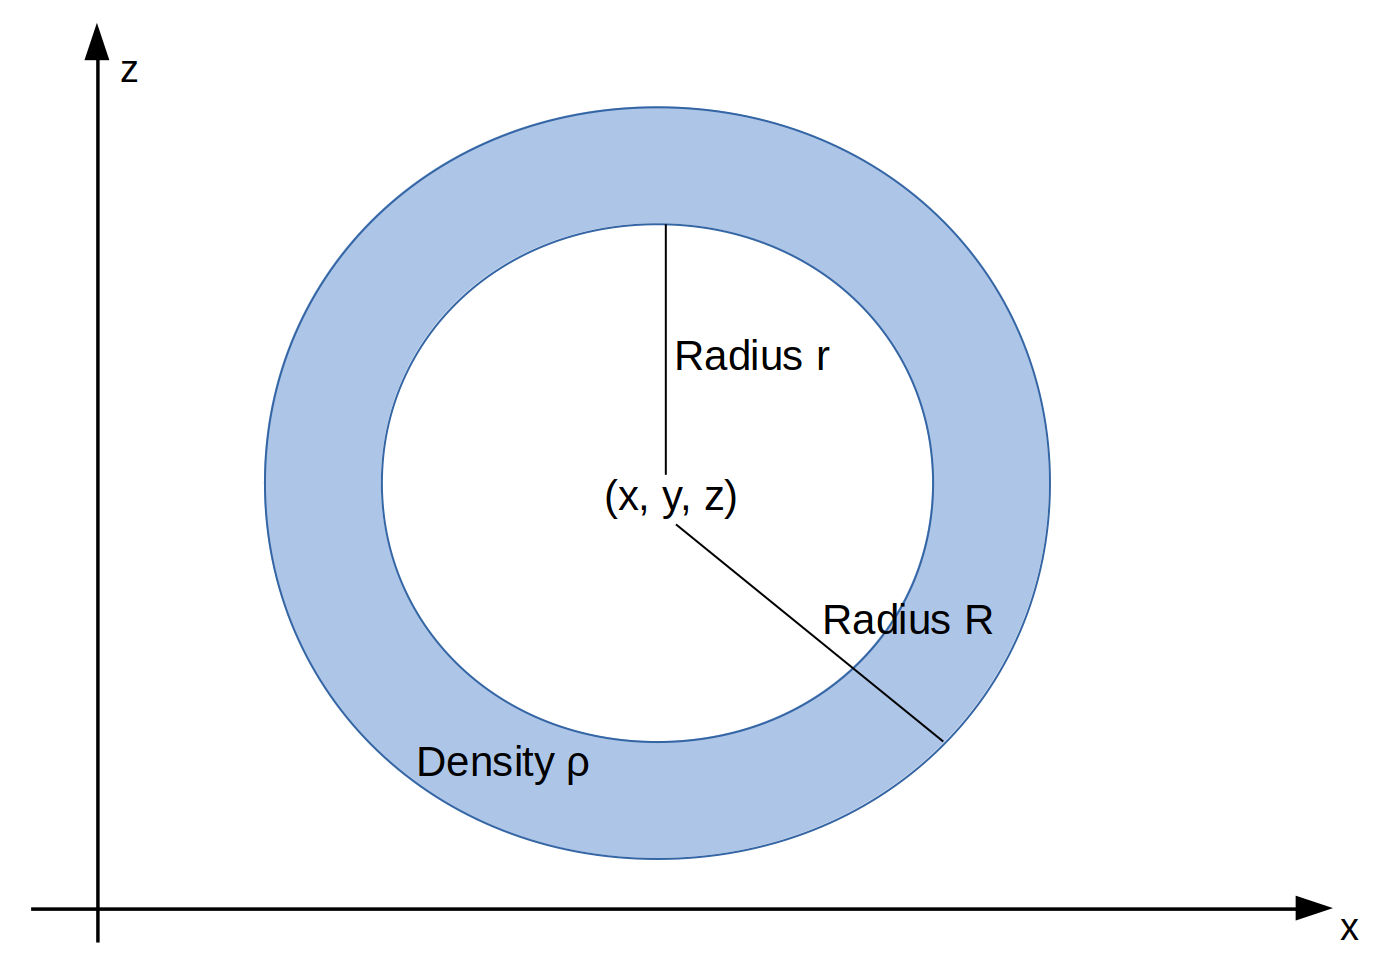
\includegraphics[width=8.5cm, height=6cm]{figs/cylinder.png}
\end{minipage}\hfill
\caption{Schematic representation of the pipe considered in this work and its geometric parameters.}
\label{fig:cylinder}
\end{figure}

One method computing the exact cut point between a muonState and a Cylinder has been defined at this point as well, from the general equation of a cylinder of radius $R$ centered in ($X$, $Y = 0$, $Z$) (given the fact that the y-axis is defined along the cylinder, we can assume that the cylinder is actually centered in $Y = 0$ without any loss of generalization).

\begin{equation}
\label{eq:cylinder}
(x - X)^2 + (z - Z)^2 = R^2
\end{equation}

From this, computing the intersection between such cylinder and a general MuonState ($x_0$, $y_0$, $z_0$, $v_{x}$, $v_{y}$, $v_{z}$, $p$) is trivial, since a MuonState can be represented with a straight line: 

\begin{equation}
\label{eq:line}
\begin{dcases}
x = x_0 + \lambda v_x \\
y = y_0 + \lambda v_y \\
z = z_0 + \lambda v_z
\end{dcases}
\end{equation}

By putting this into the equation of the cylinder, we get the following expressions:

\begin{equation}
\label{eq:together}
%\begin{dcases}
(x - X)^2 + \left (z_0 + \frac{v_z}{v_x} (x - x_0) - Z \right )^2 = R^2 \\
%x^2  - 2 x X + X^2 + z_0^2 + \left ( \frac{v_z}{v_x} \right )^2 (x-x_0)^2 + Z^2 - 2 z_0 Z -2 \frac{v_z}{v_x} (x - x_0) Z + 2 z_0 \frac{v_z}{v_x} (x - x_0) = R^2
%\end{dcases}
\end{equation}

Once both the squared values applied, we get an equation having the shape $Ax^2 + Bx + C = 0$, where both cutting points will be given therefore by $x^{+/-} = \frac{-B \pm \sqrt{B^2 - 4 AC}}{2A}$:

\begin{equation}
\label{eq:lines}
\begin{dcases}
A = \left (1 + \left (\frac{v_z}{v_x} \right )^2 \right ) \\
B = -2X - 2 x_0 \left (\frac{v_z}{v_x} \right )^2 + (2 z_0 - 2) \left (\frac{v_z}{v_x} \right ) \\
C = X^2 + Z^2 + z_0^2 - 2 z_0 Z + x_0^2 \left (\frac{v_z}{v_x} \right )^2 + x_0 (2 Z - 2 z_0) \left (\frac{v_z}{v_x} \right ) - R^2
\end{dcases}
\end{equation}

Finally, one method allowing us to determine whether a muon state is inside or outside of the pipe have also been written, taking into account the particular geometry of such objects. This is important mainly because the equation for the multiple scattering process highly depends on the density of the medium of propagation, which changes by a factor $\sim10^4$ depending on whether the muon is propagating through the steel pipe or air.

\subsection{Propagator}

A \textbf{Propagator} is then defined as the object allowing us to propagate a MuonState through a general Volume. The way it works is quite simple: 

\begin{itemize}
\item First of all, the distance between the initial MuonState and all the surfaces of the Volume considered is computed and the first intersection point is kept.
\item The muon is then propagated in a distance corresponding to 90\% of the total distance to this first cut point by taking into account the multiple scattering effect and the Moli\`ere theory, and a new MuonState is therefore obtained. We cannot propagate the muon 100\% of the distance immediately to avoid effects related to the actual shape of the Cylinder and due to the fact that the Equation~\ref{eq:Moliere} is only valid in case of normal incidence between the MuonState and the Cylinder, which is typically not verified, as shown in Figure~\ref{fig:normal}. Indeed, in this last Figure, we can see that if the normal incidence is not verified, then the width of pipe will be dependant on the deviation applied to the muon, which cannot be easily computed.

\begin{figure}[htbp]
\centering
\begin{minipage}[b]{.49\textwidth}
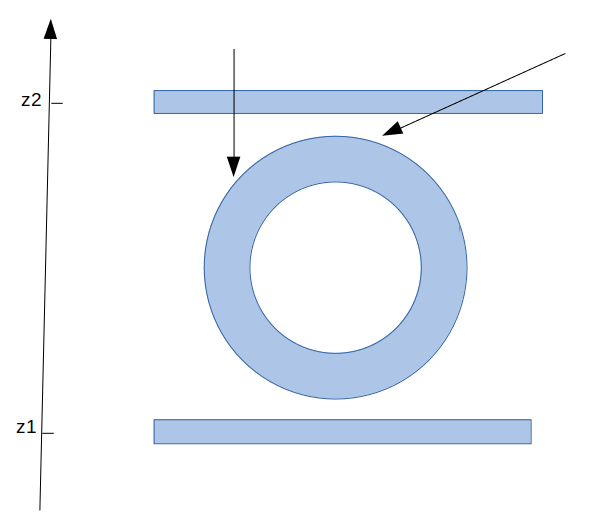
\includegraphics[width=7cm, height=6cm]{figs/normal.png}
\end{minipage}\hfill
\caption{Typical example of two incident muons not respecting the normal incidence required by the Moli\`ere equation for the multiple scattering of muons.}
\label{fig:normal}
\end{figure}

\item This propagation process is then repeated several times, until reaching a position extremely close to the volume that is being studied (our tolerance parameter has been fixed to $0.1$ mm). The muon is then manually propagated along its direction of propagation along a distance of 0.1 mm in order to force its crossing with respect to the first surface, so that the propagation process can be repeated for the next surface.
\item This whole process is repeated for all the different surfaces encountered by the muon (up to four times in total for our particular geometry), and one final time until reaching the bottom detector. At this point, the MuonState obtained is kept as the second measurement ($x_2$, $y_2$, $z_2$, $v_{x2}$, $v_{y2}$, $v_{z2}$, $p_2$) that will be compared with the simulation using statistical methods.
\item Eventual muons which do not actually crossing the pipe or which are out of the acceptance of any of the detectors are of course rejected at this stage and simply not considered.
\end{itemize}

\subsection{Likelihood}

The \textbf{Likelihood} object itself can then be calculated. This class takes as input a pipe geometry and a file containing a set of measurements (either obtained from Monte-Carlo or actually measured by the detectors) and its main objective is to estimate how likely it is that we obtained exactly these measurements for the geometry given. 

To reach this goal, several calculations are performed for each event found in the input file: 
\begin{itemize}
\item First of all, three MuonStates are computed: the so-called \textit{IncomingMuon} and \textit{OutgoingMuon}, directly read as the measurement at the upper and lower detectors from the input file, and the \textit{IncomingMuonLinearDown}, defined as the prolongation along a straight line of the \textit{IncomingMuon}. Each \textit{IncomingMuon} is then propagated along the geometry using our Propagator, defining a fourth and final \textit{IncomingMuonDown} MuonState, as shown in Figure~\ref{fig:parameters}.

\begin{figure}[htbp]
\centering
\begin{minipage}[b]{.49\textwidth}
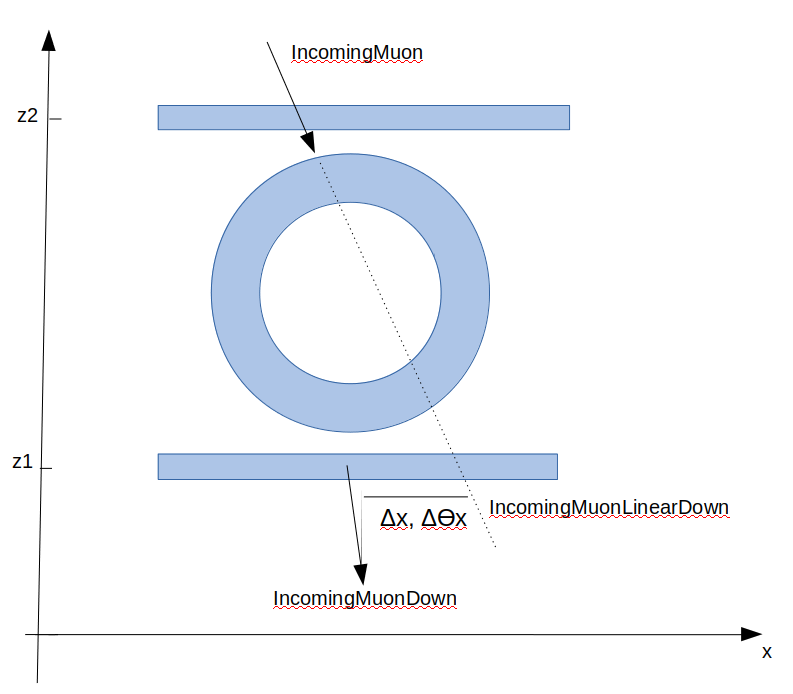
\includegraphics[width=7cm, height=6cm]{figs/parameters.png}
\end{minipage}\hfill
\caption{Schematic representation of the 4 four muonStates and main parameters used for the computation of the likelihood.}
\label{fig:parameters}
\end{figure}

\item From these muonStates, the $\Delta$x, $\Delta \theta_x$, $\Delta$y and $\Delta \theta_y$ parameters can easily be computed as the difference between the positions and angles measured between the \textit{IncomingMuonDown} and \textit{IncomingMuonLinearDown} muonStates. Such parameters are important and will be used a lot in this work since they represent the actual deviation suffered by the muon.
\item This propagation process is repeated multiple times ($N_{\text{it}} \sim 100-500$ times in total) since we known that the multiple scattering is a stochastic process. In each iteration of the loop, two bi-dimensional histograms ($\Delta$x vs $\Delta \theta_x$ and $\Delta$y vs $\Delta \theta_y$) are then filled with the actual values of the deviation parameters previously obtained.
\item Keeping in mind that this process needs to be repeated for every single event found in the input file, and given the relatively high number of iterations needed to get statistically meaningful results for each event, the kernel density estimation method introduced in Section~\ref{sec:KDF} becomes really helpful at this point. Indeed, this method allows us to keep the number of iterations (and therefore the computing time) to a minimum, while still obtaining smooth enough results to compute p-values in a reliable way.
\item At this stage, all the ingredients needed to compute a the likelihood are available. A value for each \textit{IncomingMuon} is then computed by using estimating the value of the bi-dimensional PDF from the histograms previously defined and representing all the possible deviation values for a single event, and by comparing the actual measurement \textit{OutgoingMuon} to such distributions.
\item Two values, one along each of the $x$ and $y$ axes, are then obtained using this method for each of the $N$ events found in the input file. The total value returned by this function can then simply be computed from Equation~\ref{eq:totallikelihood}.

\begin{equation}
\label{eq:totallikelihood}
\mathcal{L} = \left( \frac{1}{N} \right) \sum_{i = 1}^N -2.0 \left ( \log(\text{pvalue}_{x, i}) + \log(\text{pvalue}_{y, i}) \right)
\end{equation}

%Given the relative complexity of the different computation steps performed in this class, the steps previously defined can be summarized in the following pseudocode.

%\begin{verbatim}
%for each event in input file

%    IncomingMuon = top position and direction MuonState
%    OutgoingMuon = bottom position and direction MuonState
%    IncomingMuonLinearDown = linear propagation of IncomingMuon to bottom detector
    
%    for each iteration
%        IncomingMuonDown = IncomingMuon propagated to bottom detector
%        measX = IncomingMuonDown.getX() - IncomingMuonLinearDown.getX()
%\end{verbatim}

%\item So far, we described a method allowing to compute the likelihood of observing a given measurement by using Monte-Carlo simulations for a given volume, but one last important step is still missing: we need to find a way to find the optimal volume for a given measurement, the main objective of this process. 
%\color{red} Talk about the minimization process once implemented. \color{black}
\end{itemize}

\section{Generator} \label{sec:Generator}

As we have just seen, the computation of the values required for the likelihood takes as input a file of Monte-Carlo generated events, which needs to be previously produced thanks to Geant4 or to this \textbf{Generator}, assuming a perfect detector but typically orders of magnitude faster. This class takes as input one rootfile containing the Monte-Carlo generation of incoming cosmic muons previously produced by the company using CRY \cite{CRY}, a dedicated generator for cosmic muons. To simplify the current problem, the goal is then to simply read the input parameters of such muons, such as the position of their impact with the upper detector, and to propagate them using the previously defined functions, to generate a distribution of the expected output.

The way this algorithm works is quite simple: a general volume matching the one that needs to be studied (in this case, a general Pipe located in the center (0, 0, 0) of the detector, having an inner radius variable, an outter radius of 20 cm and a length of 50 cm) is first of all defined. Then, for each event we want to generate ($n_{\text{MC}} \sim 10.000$), a loop is performed: in each iteration of this loop, the incident muon is propagated throughout the geometry, histograms for the parameters $\Delta x$, $\Delta \theta_x$, $\Delta y$ and $\Delta \theta_y$ are obtained and, more importantly, measurements in the lower detector are artificially generated to test our framework without having to consider detector effects for now.

One last important notion to introduce at this point is the difference between the actual measurement and the Monte-Carlo truth value, that can both be computed by the generator. The existence of both variables is related to the fact that the detector is made out of 200 discrete wires, each separated by a distance of 4 mm, meaning that the actual position measured is typically a discrete number. However, when considering simulation files, both the real and the measured position can be obtained and kept in different MuonStates labelled as ($px_i$, $py_i$, $pz_i$, $pv_{xi}$, $pv_{yi}$, $pv_{zi}$, $p_i$) and ($mx_i$, $my_i$, $mz_i$, $mv_{xi}$, $mv_{yi}$, $mv_{zi}$, $m_i$) respectively. Depending on whether we are working with Monte-Carlo simulations or data, one or the other MuonState will then be chosen.

\section{Plotter} \label{sec:Plotter}

Finally, the last important ingredient of the framework built is the Plotter, allowing us to plot different results obtained. This part of the framework is therefore able to:

\begin{itemize}
    \item Simply plot the position, direction and deviation parameters $\Delta x$, $\Delta \theta_x$, $\Delta y$ and $\Delta \theta_y$ of the MuonStates measured at the top and bottom detectors, by reading the rootfile containing either data or Monte-Carlo generated from the Generator.
    \item Draw on the same canvas all these parameters for two different generators at once, allowing us to compare the results of our Generator with the results obtained from a full Geant4 simulation, in order to validate this framework.
    \item Plot on the same canvas the deviation parameters obtained by considering different pipe geometries to compare them.
    \item Generate 2D distributions representing the results obtained by the kernel density estimator method to check them and make sure the smoothing process works as expected.
    \item Finally, plot all the likelihood curves obtained by considering different input files and pipe geometries, allowing us to graphically minimize this likelihood and therefore find the most likely geometry for each of the generated files.
\end{itemize}

All this framework has been developed internally for the specific use of the company MuonSystems and is therefore unfortunately not available in a public repository.










































\chapter{Results obtained} \label{chapter:results}

Now that the experimental setup and main statistical parameters used have been fully described and that the algorithm developed for this particular exercise has been introduced, we can present the results obtained. This chapter is divided into several sections: first of all, we are going to mention the different validation steps performed to make sure that this algorithm's results can be trusted in Section~\ref{sec:validation} and then, more general results obtained for different pipe geometries will be presented in Section~\ref{sec:general}, along with the final likelihood results of this work.

\section{Generator validation} \label{sec:validation}

The validation step consists in comparing the results previously obtained with Geant4, a a toolkit for the simulation of the passage of particles through matter \cite{Geant4}, with a complete and realistic description of the interaction between the cosmic muons and the detectors, and the ones obtained with our Generator, assuming a perfect detector but typically orders of magnitude faster.

This step is actually extremely important, as it allowed us to find several bugs in the code. In this context, several files have been generated using both generators and different pipe geometries, allowing us to perform several different checks. In each case, the objective was to obtain the output MuonState ($x_2$, $y_2$, $z_2$, $v_{x2}$, $v_{y2}$, $v_{z2}$, $p_2$) after propagating the initial MuonState throughout a given geometry.

For a given pipe having a geometry ($r = 17.2$ cm, $R = 20$ cm, $L = 50$ cm) and located in (0, 0, 0), thousands of muons have then been generated using both Geant4 and our Generator. The output distributions (the positions $x$ and $y$ and directions $v_x$ and $v_y$ after propagation, along with the deviations in position $\Delta$x and $\Delta$y, defined in Equation\ref{eq:deviationPos} where $d$ is the vertical distance between the two detectors, and the angular deviation $\Delta \theta_x$ and $\Delta \theta_y$, defined in Equation~\ref{eq:deviationDir}) have then been obtained in this case in Figure~\ref{fig:genComp}. All these plots have been normalized to unity in order to account for the eventual different number of events generated with both generators.

\begin{equation}
\label{eq:deviationPos}
\begin{dcases}
\Delta \text{x} = x_2 + d (v_{x2} - x_1)  \\
\Delta \text{y} = y_2 + d (v_{y2} - y_1)
\end{dcases}
\end{equation}

\begin{equation}
\label{eq:deviationDir}
\begin{dcases}
\Delta \theta_x = \arctan \left ({\frac{v_{x2}}{v_{z2}}} \right ) - \arctan \left ({\frac{v_{x1}}{v_{z1}}} \right ) \\
\Delta \theta_y = \arctan \left ({\frac{v_{y2}}{v_{z2}}} \right ) - \arctan \left ({\frac{v_{y1}}{v_{z1}}} \right )
\end{dcases}
\end{equation}

\begin{figure}[htbp]
\centering
\subfigure[Muon position (on the left) and direction (on the right) along the x-axis at the bottom detector after propagation]
 {
\begin{minipage}[b]{.49\textwidth}
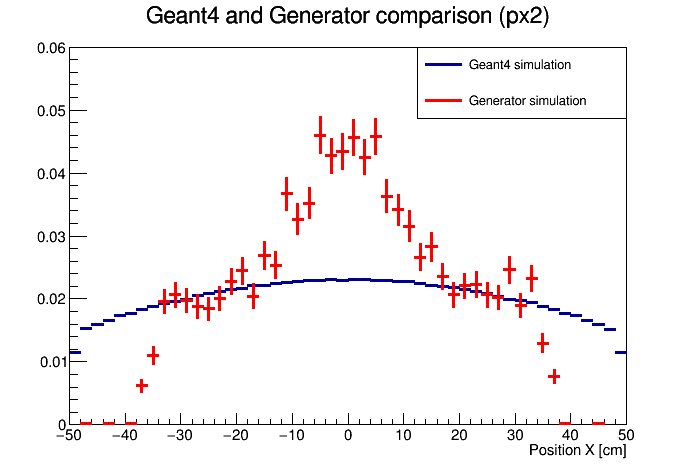
\includegraphics[width=8cm, height=6cm]{figs/px2-17p2vs17p2.png}
\end{minipage}\hfill
\begin{minipage}[b]{.49\textwidth}
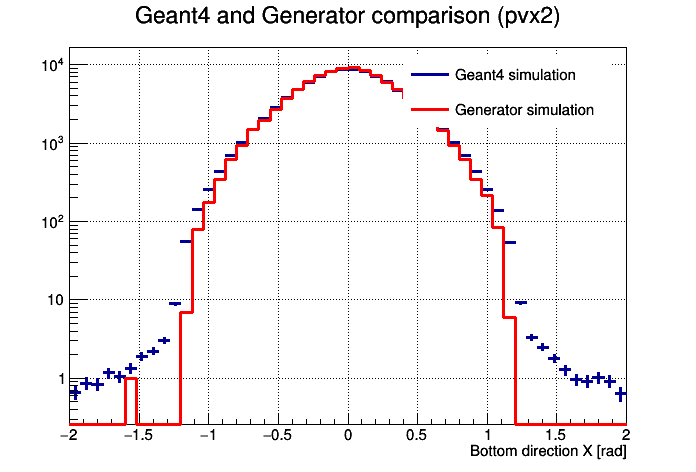
\includegraphics[width=8cm, height=6cm]{figs/pvx2-17p2vs17p2.png}
\end{minipage} \hfill
}
\subfigure[Muon $\Delta$x (on the left) and $\Delta$y (on the right) as measured after propagation]
 {
\begin{minipage}[b]{.49\textwidth}
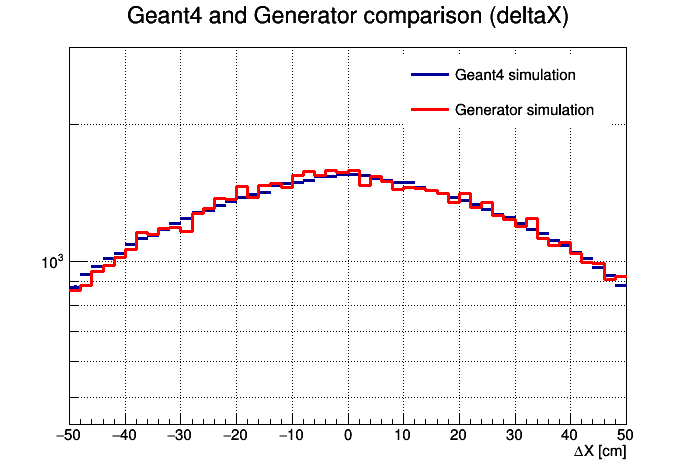
\includegraphics[width=8cm, height=6cm]{figs/deltaX-17p2vs17p2.png}
\end{minipage}\hfill
\begin{minipage}[b]{.49\textwidth}
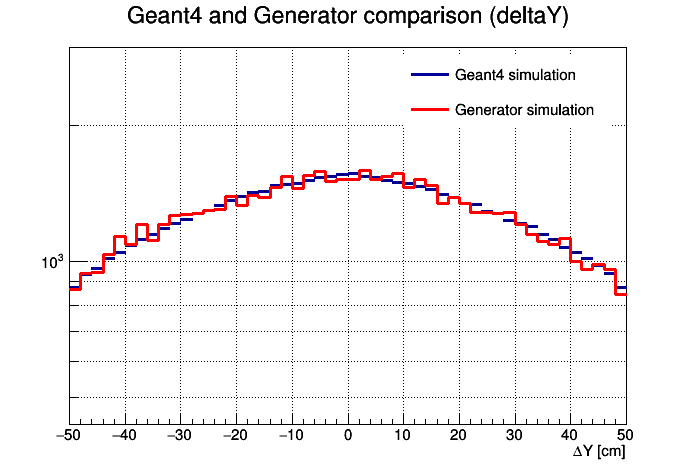
\includegraphics[width=8cm, height=6cm]{figs/deltaY-17p2vs17p2.png}
\end{minipage} \hfill
}
\subfigure[Muon $\Delta \theta_x$ (on the left) and $\Delta \theta_y$ (on the right) as measured after propagation]
 {
\begin{minipage}[b]{.49\textwidth}
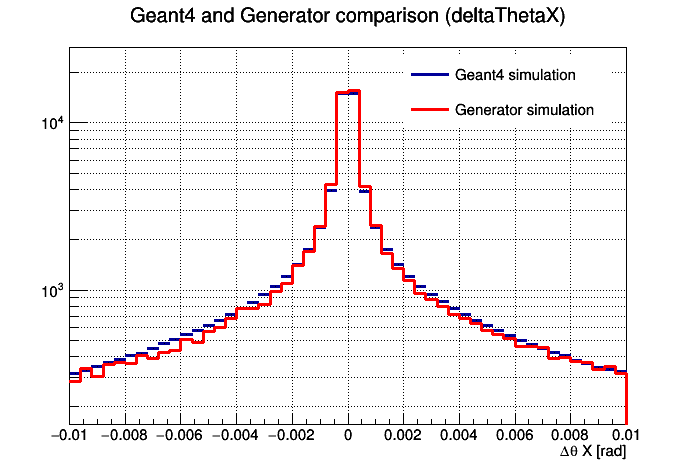
\includegraphics[width=8cm, height=6cm]{figs/deltaThetaX-17p2vs17p2.png}
\end{minipage}\hfill
\begin{minipage}[b]{.49\textwidth}
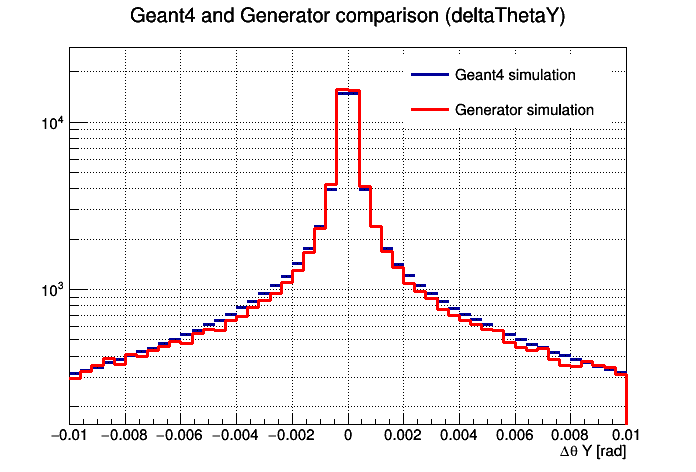
\includegraphics[width=8cm, height=6cm]{figs/deltaThetaY-17p2vs17p2.png}
\end{minipage} \hfill
}
\caption{Normalized variables measured on the bottom detector using the Geant4 (in blue) simulation process and our custom Generator (in red).}
\label{fig:genComp}
\end{figure}

%\section{Cosmic muons properties} \label{sec:incident}

%One of the most famous properties of cosmic muons is their regular angular distribution $T_\theta$, given by Equation~\ref{eq:cossquare}, where $p_0$ and $p_1$ are parameters depending on several factors, such as the altitude and latitude of the place where the measurement is performed.

%\begin{equation}
%\label{eq:cossquare}
%I_\theta = p_0 \cos^{p_1} \theta \propto cos^{p_1} \theta
%\end{equation}

%At our latitude, we can approximately estimate that $p_1 \simeq 2$ and this is something we can easily check with our experimental setup, given the fact that the upper detector is able to give us such angular distribution from a simple fit. Another important property of cosmic muons is their relatively well known vertical energy spectrum, following a power law $p_0 E^{-p_1}$ \cite{properties}, that we can also represent here, in order to check for the validity of the cosmic muons generated with CRY. The results obtained in both cases are shown in Figure~\ref{fig:prop}.

%\begin{figure}[htbp]
%\centering
%\begin{minipage}[b]{.49\textwidth}
%
\includegraphics[width=8cm, height=6cm]{figs/placeholder.png}
%\end{minipage}\hfill
%\begin{minipage}[b]{.49\textwidth}
%\includegraphics[width=8cm, height=6cm]{figs/incidentEnergy.png}
%\end{minipage}\hfill
%caption{Study of the angular (on the left) and energy (on the right) distributions of cosmic muons generated by CRY and used throughout this work.}
%\label{fig:prop}
%\end{figure}

\section{General results} \label{sec:general}

\subsection{Pipe geometries impact}

Now that we know we can trust the results obtained from the Generator, the next step has then been to generate 9 Monte-Carlo files with 10.000 to 50.000 events each, using our Generator, corresponding to 9 possible pipe geometries characterized by a constant length $L = 50$cm, an outer radius of $R = 20$cm and different inner radii $r$, ranging from 16.6 to 19.0cm, by steps of 0.2cm. It took 8 seconds to produce a file with 50.000 events per geometry considered, almost two orders of magnitude faster than a file generation using the Geant4 generator.

We can then start comparing the $\Delta$x, $\Delta$y, $\Delta \theta_x$ and $\Delta \theta_y$ distributions obtained for these different geometries, as shown in Figure~\ref{fig:gemComp}.

\begin{figure}[htbp]
\centering
\subfigure[Muon $\Delta$x (on the left) and $\Delta$y (on the right) as measured after propagation]
 {
\begin{minipage}[b]{.49\textwidth}
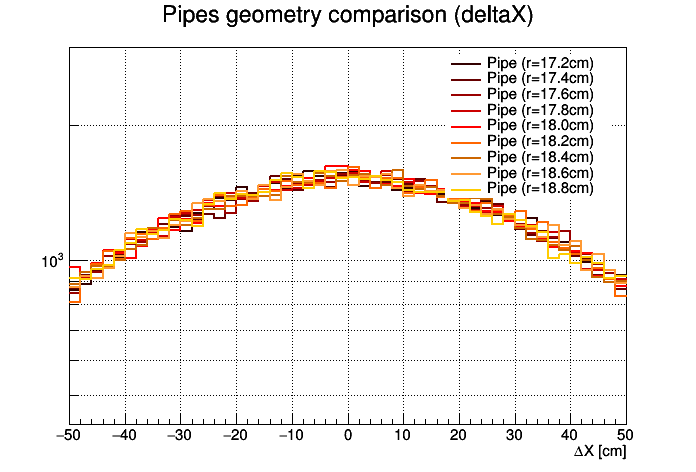
\includegraphics[width=8cm, height=6cm]{figs/deltaX.png}
\end{minipage}\hfill
\begin{minipage}[b]{.49\textwidth}
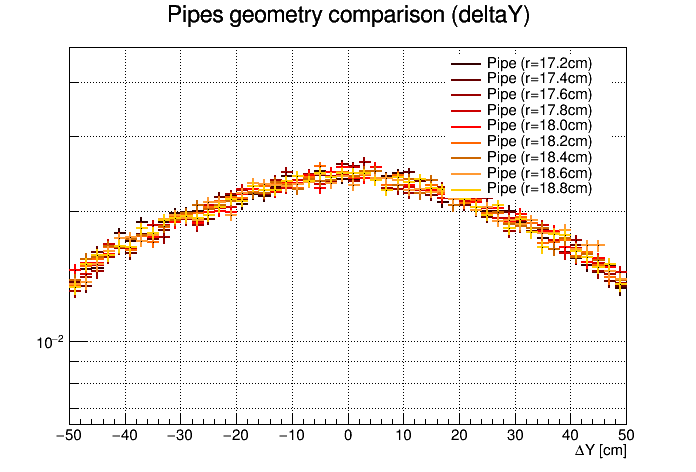
\includegraphics[width=8cm, height=6cm]{figs/deltaY.png}
\end{minipage} \hfill
}
\subfigure[Muon $\Delta \theta_x$ (on the left) and $\Delta \theta_y$ (on the right) as measured after propagation]
 {
\begin{minipage}[b]{.49\textwidth}
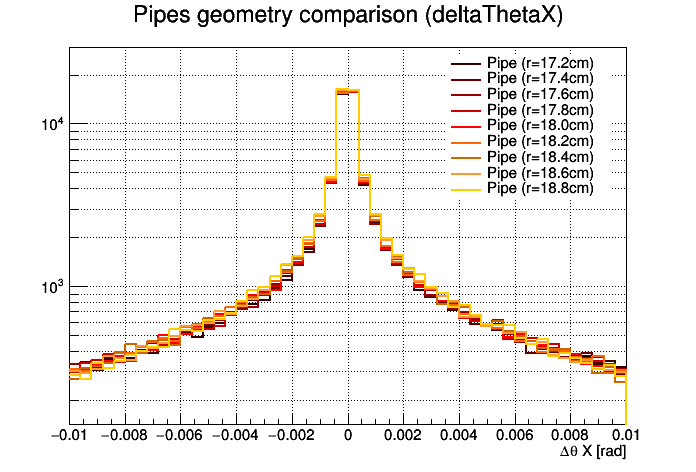
\includegraphics[width=8cm, height=6cm]{figs/deltaThetaX.png}
\end{minipage}\hfill
\begin{minipage}[b]{.49\textwidth}
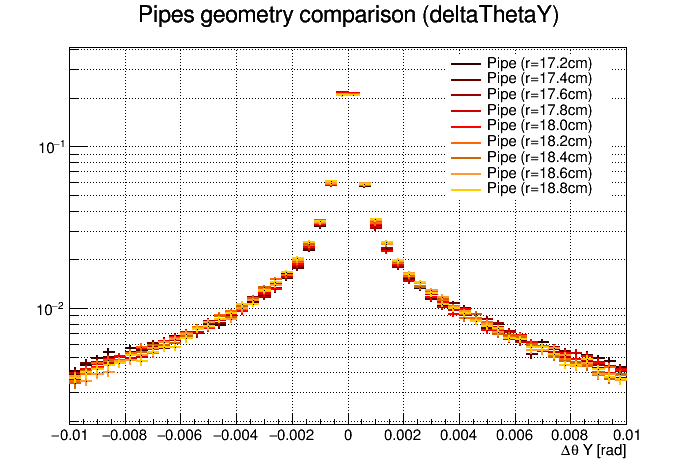
\includegraphics[width=8cm, height=6cm]{figs/deltaThetaY.png}
\end{minipage} \hfill
}
\caption{Normalized deviation variables generated using different pipe geometries.}
\label{fig:gemComp}
\end{figure}

As we can see, the geometry actually has only a little impact on the deviation observed in the position and direction, along both the $x$ and $y$ axes. We can however observe slightly larger tails for the pipes having a larger inner width, as expected. The study of these small differences between the different geometries will be the starting point of the determination of the properties of an unknown pipe placed between the two detectors using our Likelihood class.

\subsection{Kernel density functions}

As explained previously, we generated between 10.000 and 50.000 events events for each geometry with our Generator and, for every single event, a likelihood needs to be computed, which involves running another loop of at least several hundreds of iterations. In each iteration, the value of the deviation in position and angle between the MuonState obtained with our Propagator and the one defined as the linearly propagated MuonState to the bottom detector is computed, filling in this process two bi-dimensional histograms ($\Delta$x vs $\Delta \theta_x$ and $\Delta$y vs $\Delta \theta_y$) for each input event.

More precise results are expected to be obtained by increasing this number of iterations, but so does the computing time, so in order to keep the code running time manageable, we decided to use the kernel density estimation method described in Section~\ref{sec:KDF}, allowing us to reduce this number of iterations while keeping the results reliable and smooth. Both the original and the smoothen histograms obtained for a single event can be found in Figure~\ref{fig:KDFresults}.

\begin{figure}[htbp]
\begin{center}
\subfigure[($\Delta$x vs $\Delta \theta_x$) histogram along the x-axis, without (on the left) and with (on the right) smoothening applied.]
 {
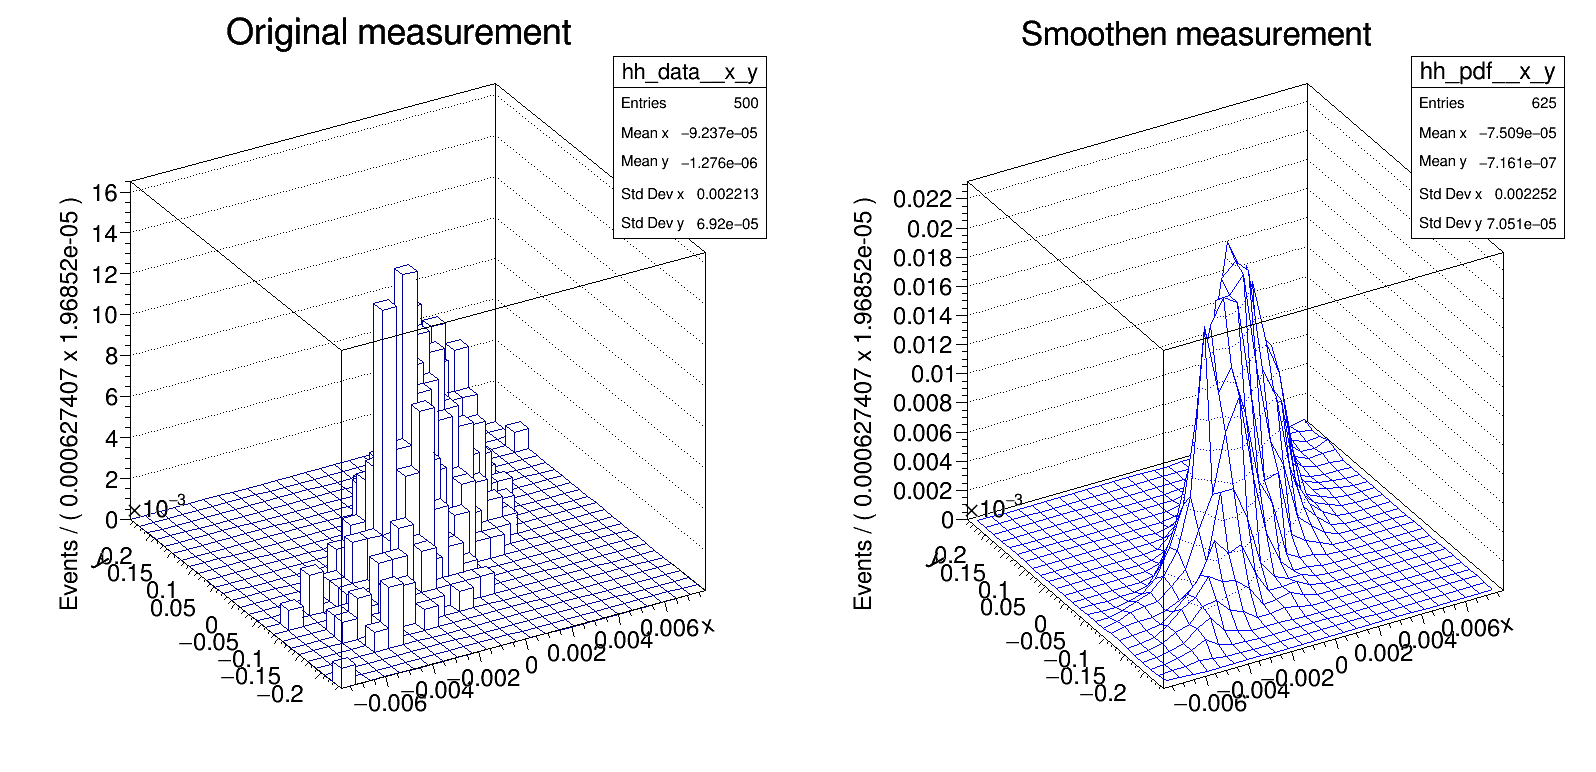
\includegraphics[width=16cm, height=7.6cm]{figs/plot_kernely.png}
}
\subfigure[($\Delta$y vs $\Delta \theta_y$) histogram along the y-axis, without (on the left) and with (on the right) smoothening applied.]
 {
 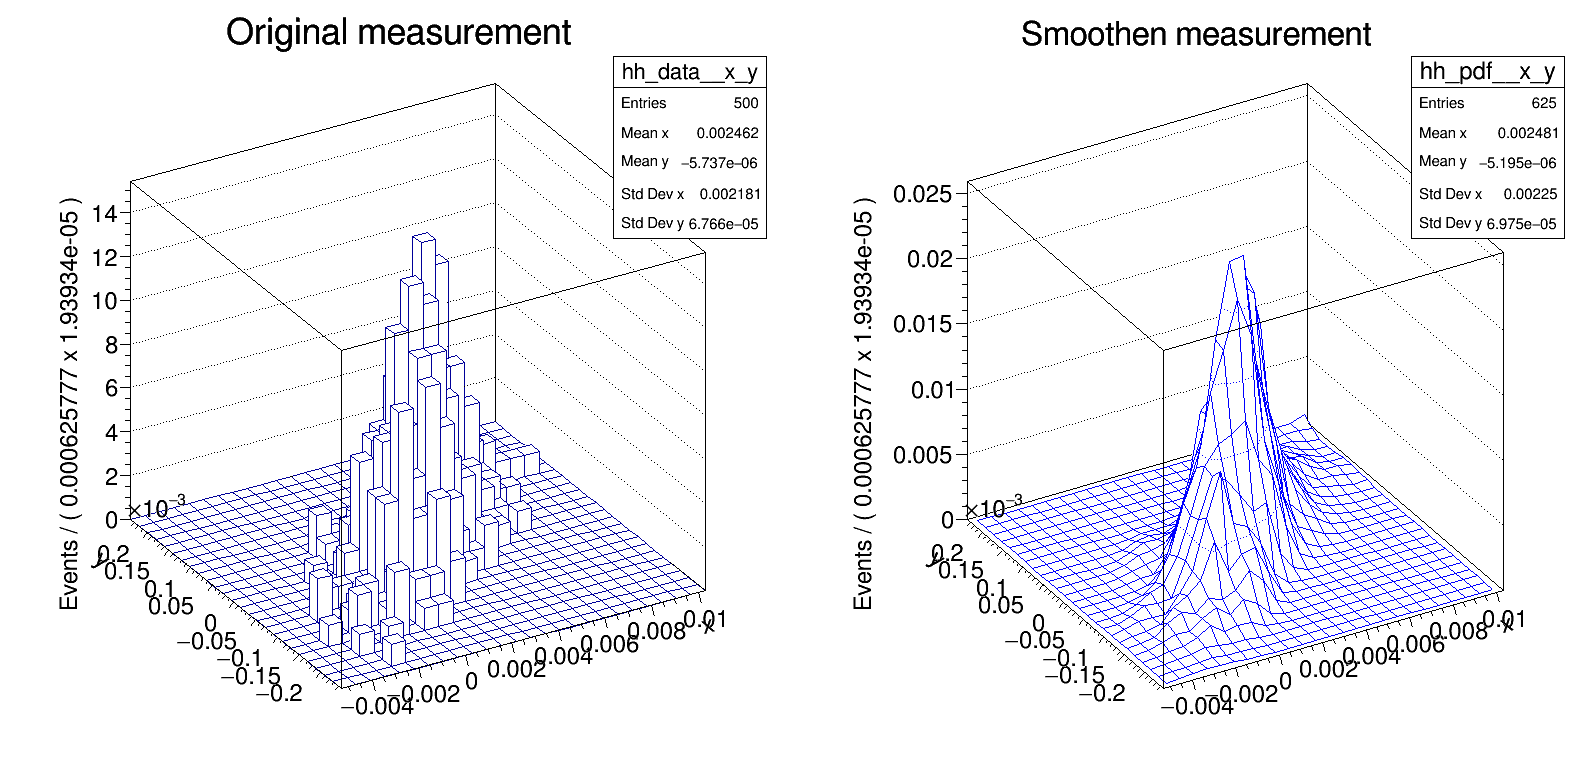
\includegraphics[width=16cm, height=7.6cm]{figs/plot_kernelx.png}
 }
\caption{Original and smoothen bi-dimensional histograms along the x and y axes, obtained for a single event generated with the Generator class.}
\label{fig:KDFresults}
\end{center}
\end{figure}

\subsection{Likelihood curves}

The goal is now to finally estimate the value of the total likelihood obtained for different pipe geometries, characterized by different inner radii, ranging from 16.6 to 19.0cm, by steps of 0.2cm.

The idea is in this sense to compute the value of the likelihood obtained for each of these geometries by comparing an actual measurement obtained with our Propagator with these generated files one by one, in order to estimate the value of the PDF and minimize the likelihood obtained in each case to, at the end of the day, try to figure out which pipe geometry is more likely to give rise to such measurements. The results obtained are shown in Figures~\ref{fig:likelihoods} for iterations of computation for the likelihood and with 10.000 events simulated, in Figure~\ref{fig:likelihoods2} for 100 iterations and 50.000 events simulated and finally in Figure~\ref{fig:likelihoods3} for 250 computation iterations and 10.000 simulated events. In all these figures, the vertical red line shows the place where we would expect to see the minimum value.

\begin{figure}[htbp]
\centering
\begin{minipage}[b]{.32\textwidth}
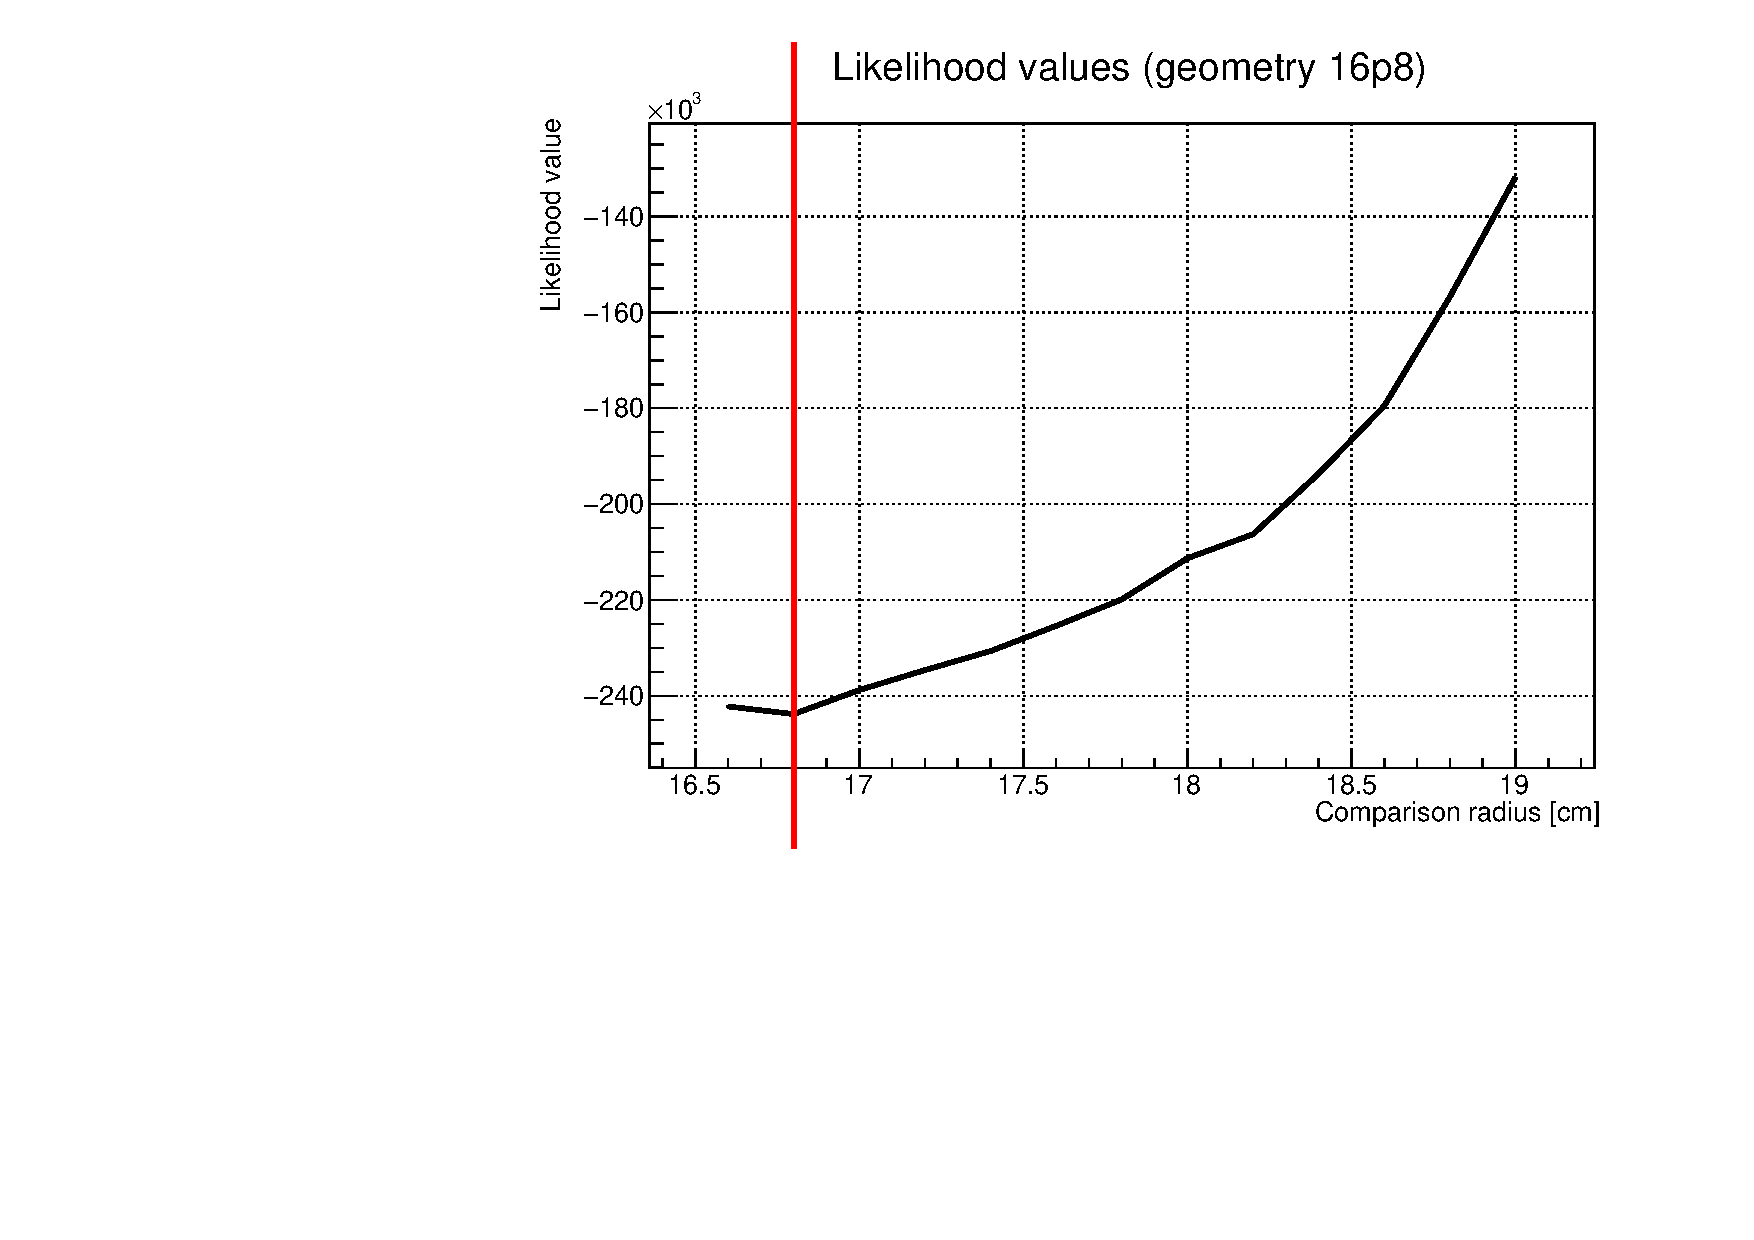
\includegraphics[width=6cm, height=4.6cm]{figs/likelihood100LowStat/likelihood16p8.pdf}
\end{minipage}\hfill
\begin{minipage}[b]{.32\textwidth}
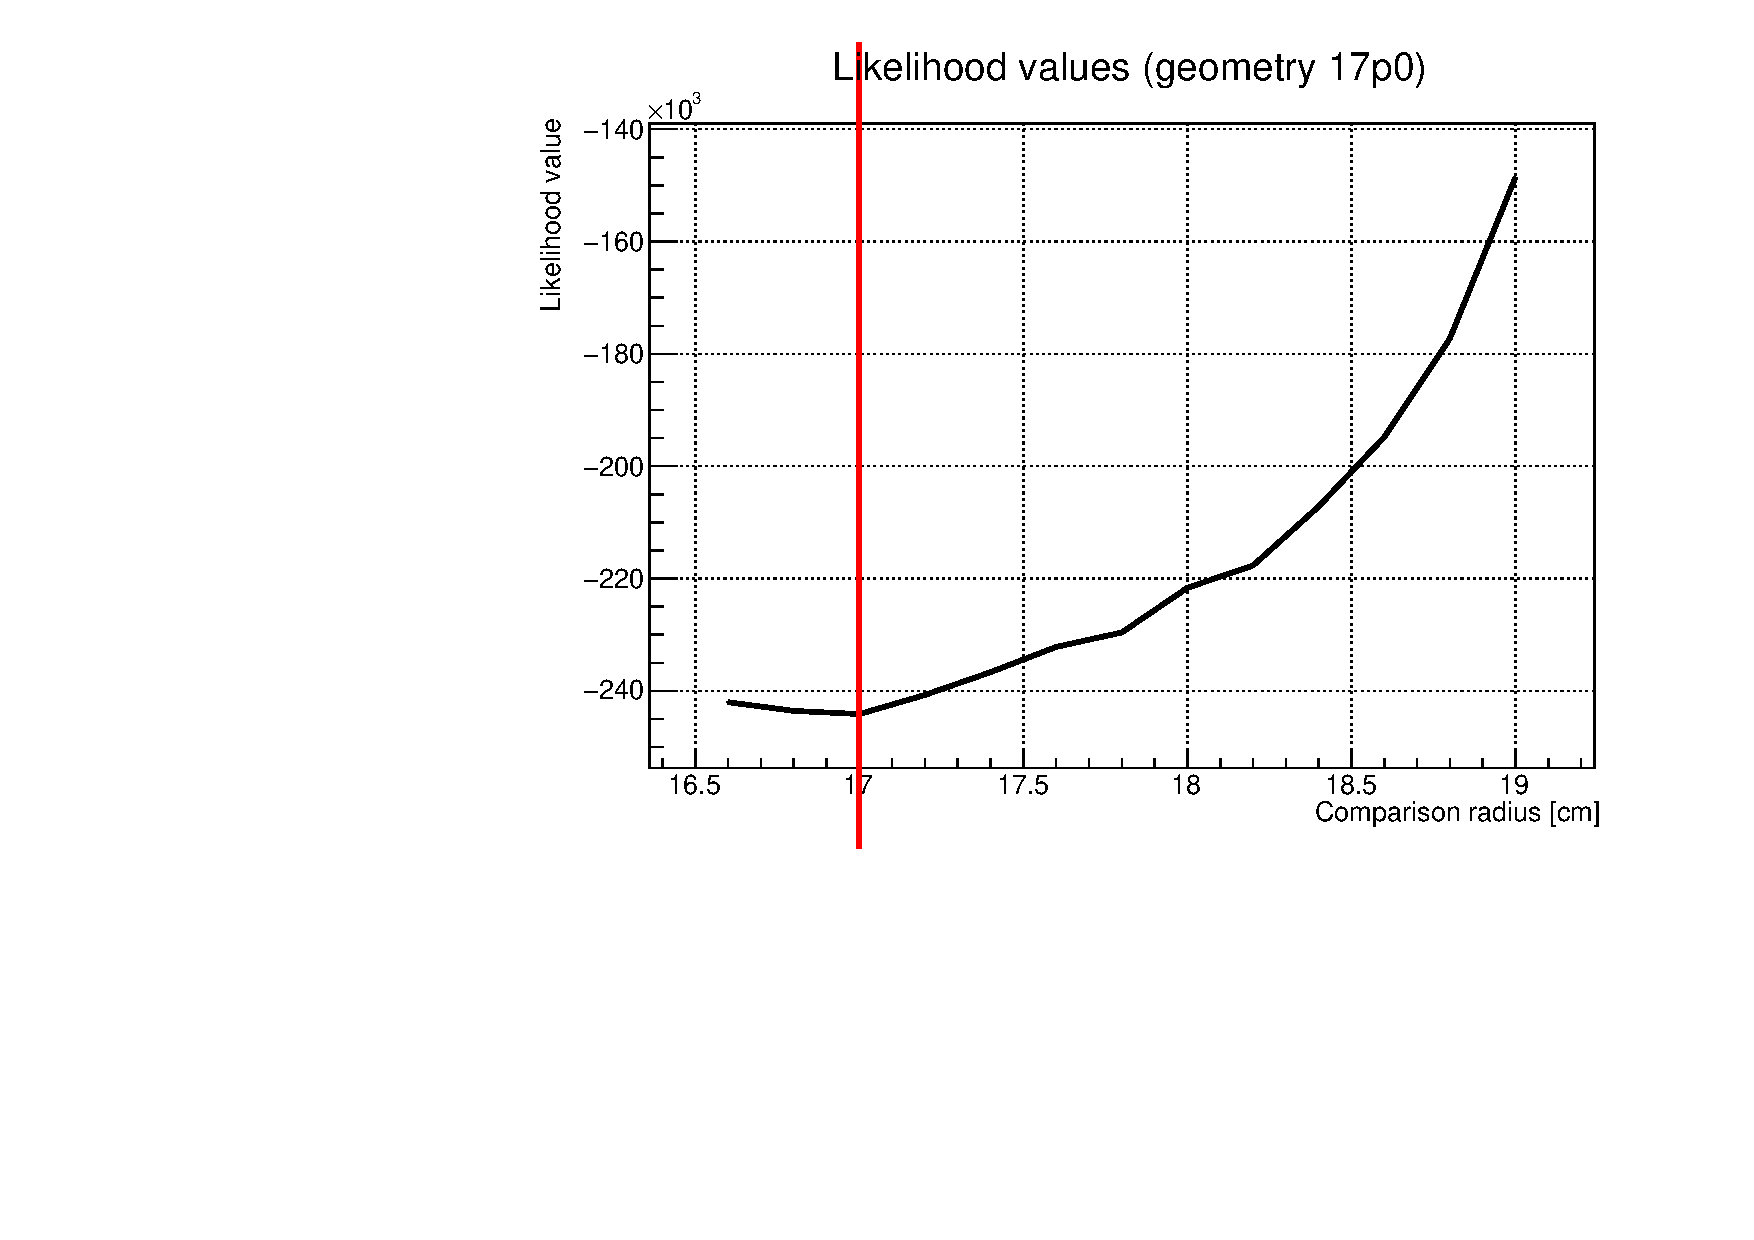
\includegraphics[width=6cm, height=4.6cm]{figs/likelihood100LowStat/likelihood17p0.pdf}
\end{minipage} \hfill
\begin{minipage}[b]{.32\textwidth}
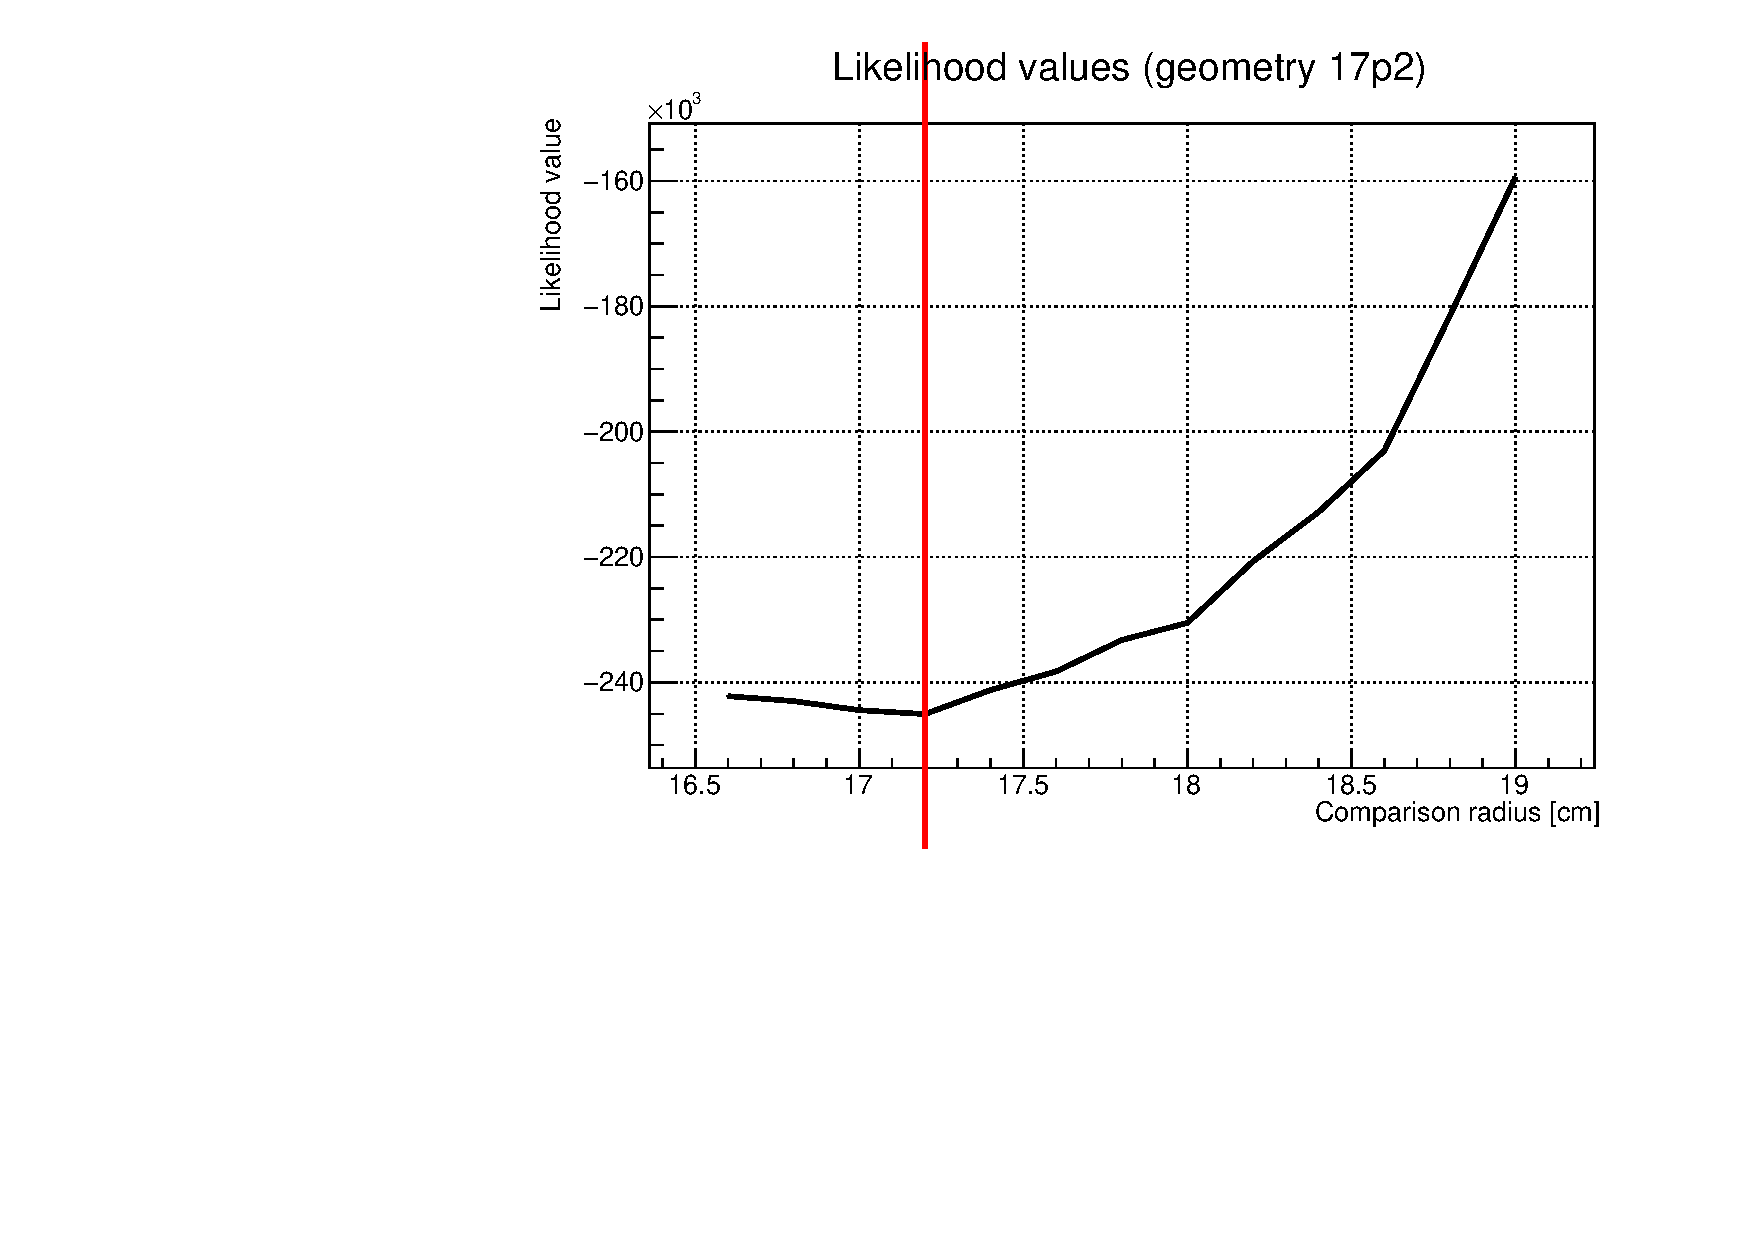
\includegraphics[width=6cm, height=4.6cm]{figs/likelihood100LowStat/likelihood17p2.pdf}
\end{minipage} \hfill \vspace{10pt}

\begin{minipage}[b]{.32\textwidth}
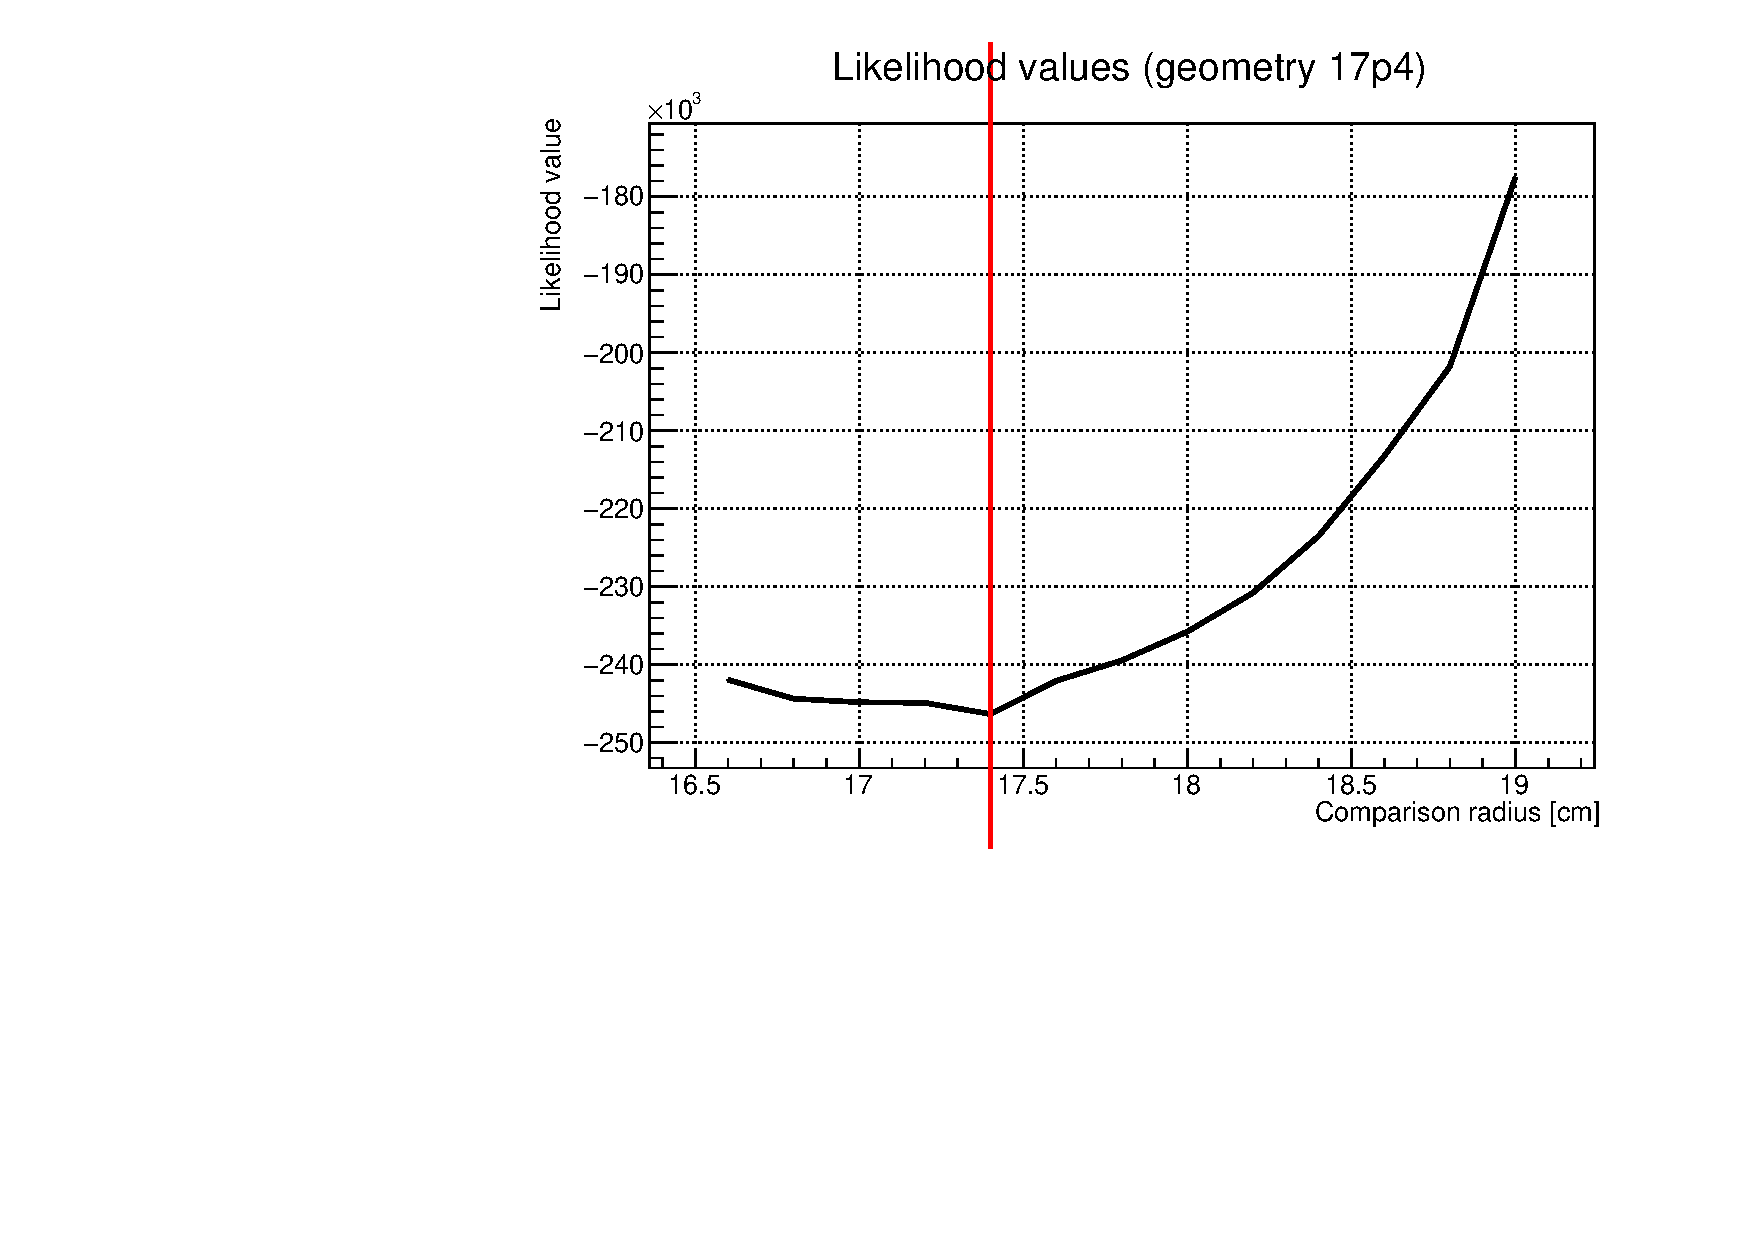
\includegraphics[width=6cm, height=4.6cm]{figs/likelihood100LowStat/likelihood17p4.pdf}
\end{minipage}\hfill
\begin{minipage}[b]{.32\textwidth}
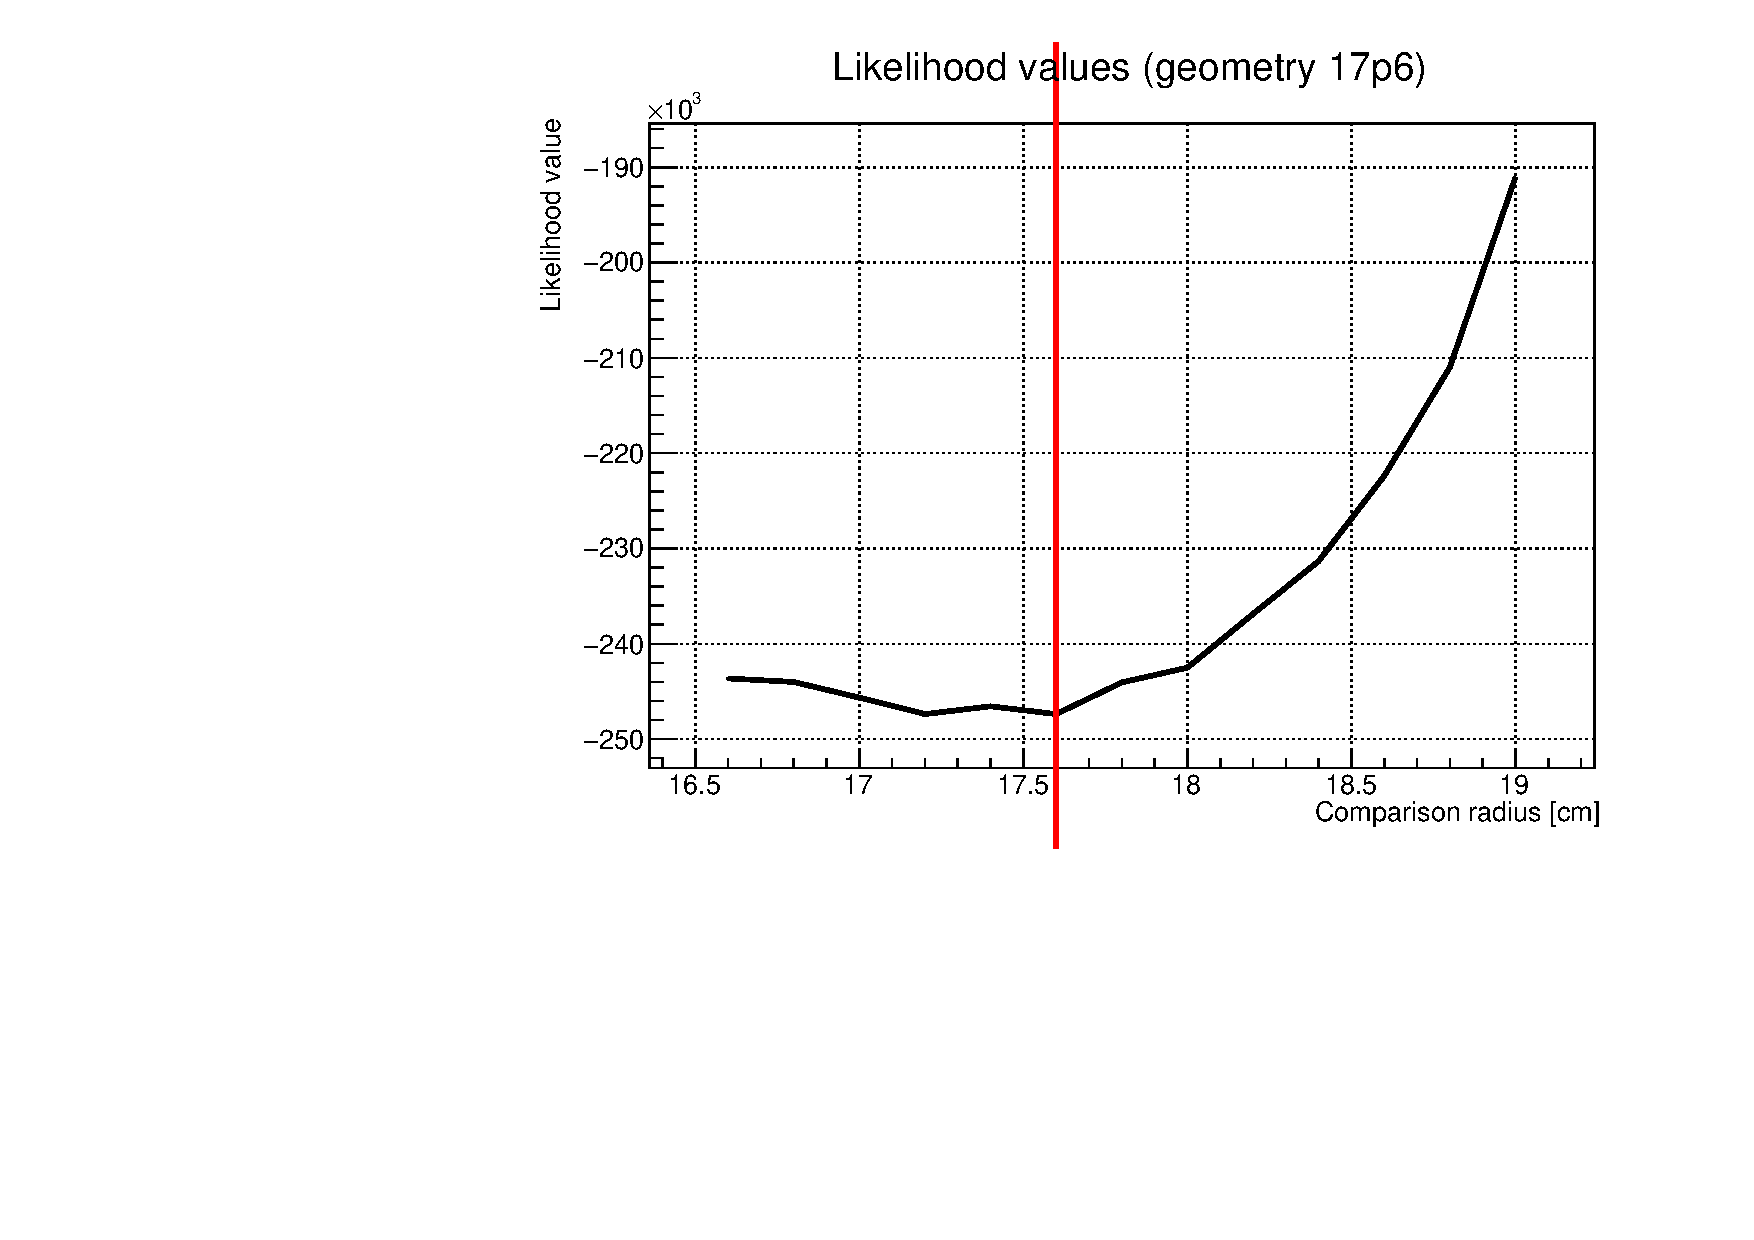
\includegraphics[width=6cm, height=4.6cm]{figs/likelihood100LowStat/likelihood17p6.pdf}
\end{minipage} \hfill
\begin{minipage}[b]{.32\textwidth}
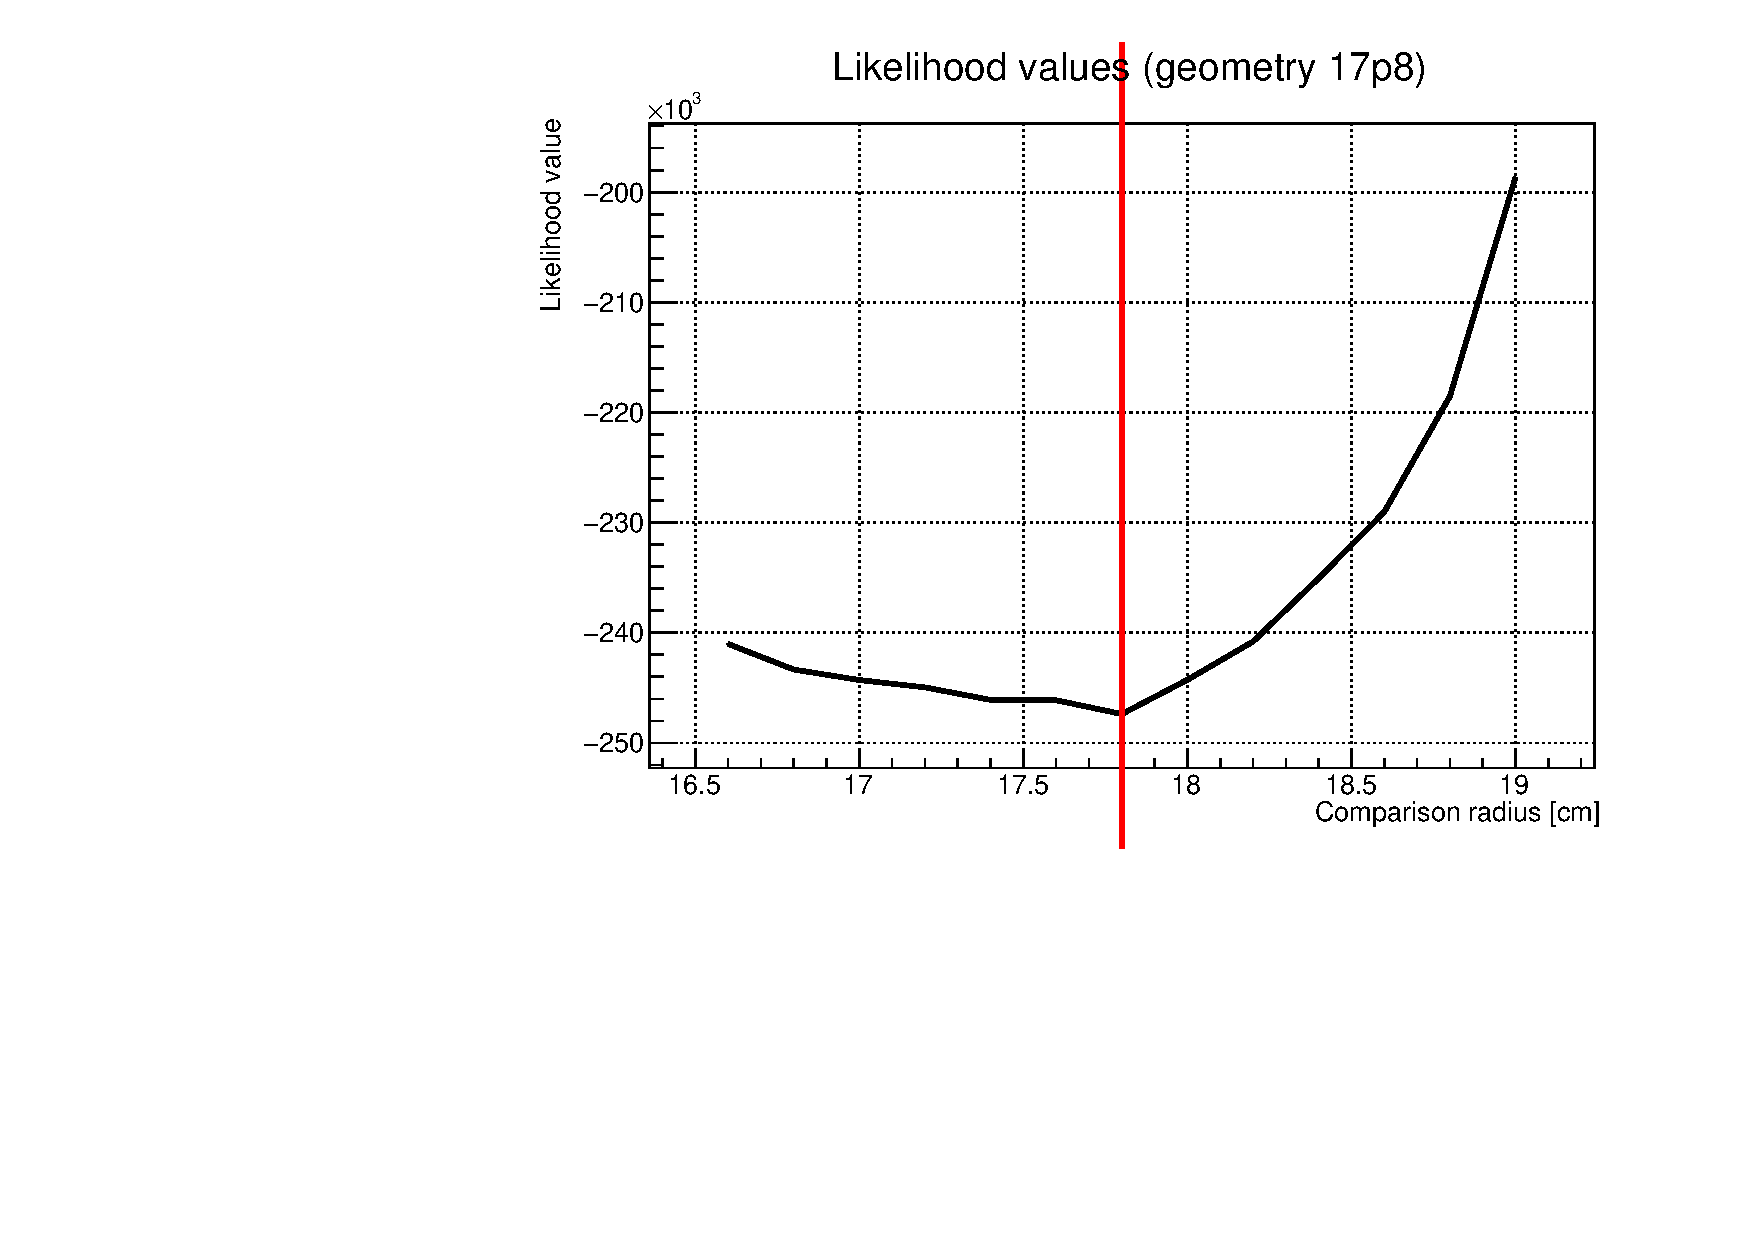
\includegraphics[width=6cm, height=4.6cm]{figs/likelihood100LowStat/likelihood17p8.pdf}
\end{minipage} \hfill \vspace{10pt}

\begin{minipage}[b]{.32\textwidth}
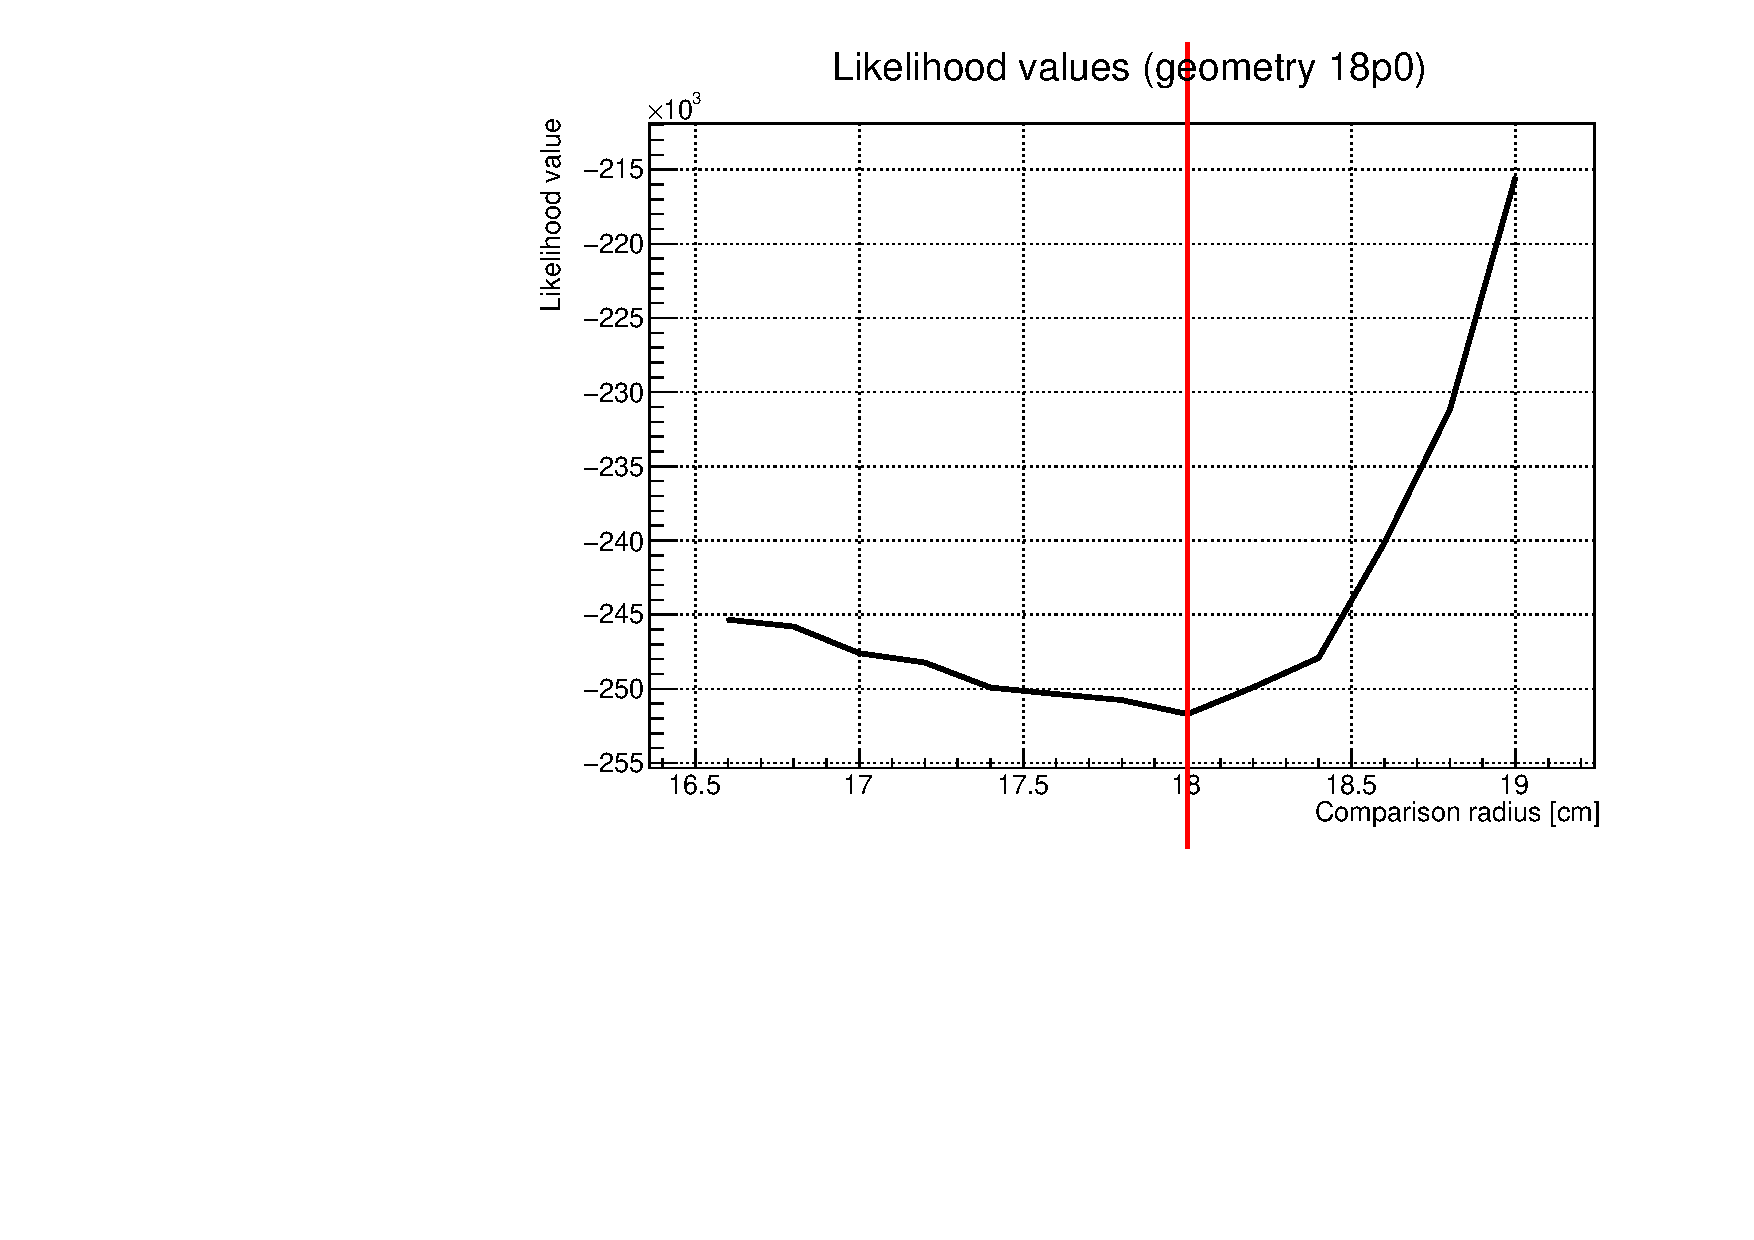
\includegraphics[width=6cm, height=4.6cm]{figs/likelihood100LowStat/likelihood18p0.pdf}
\end{minipage}\hfill
\begin{minipage}[b]{.32\textwidth}
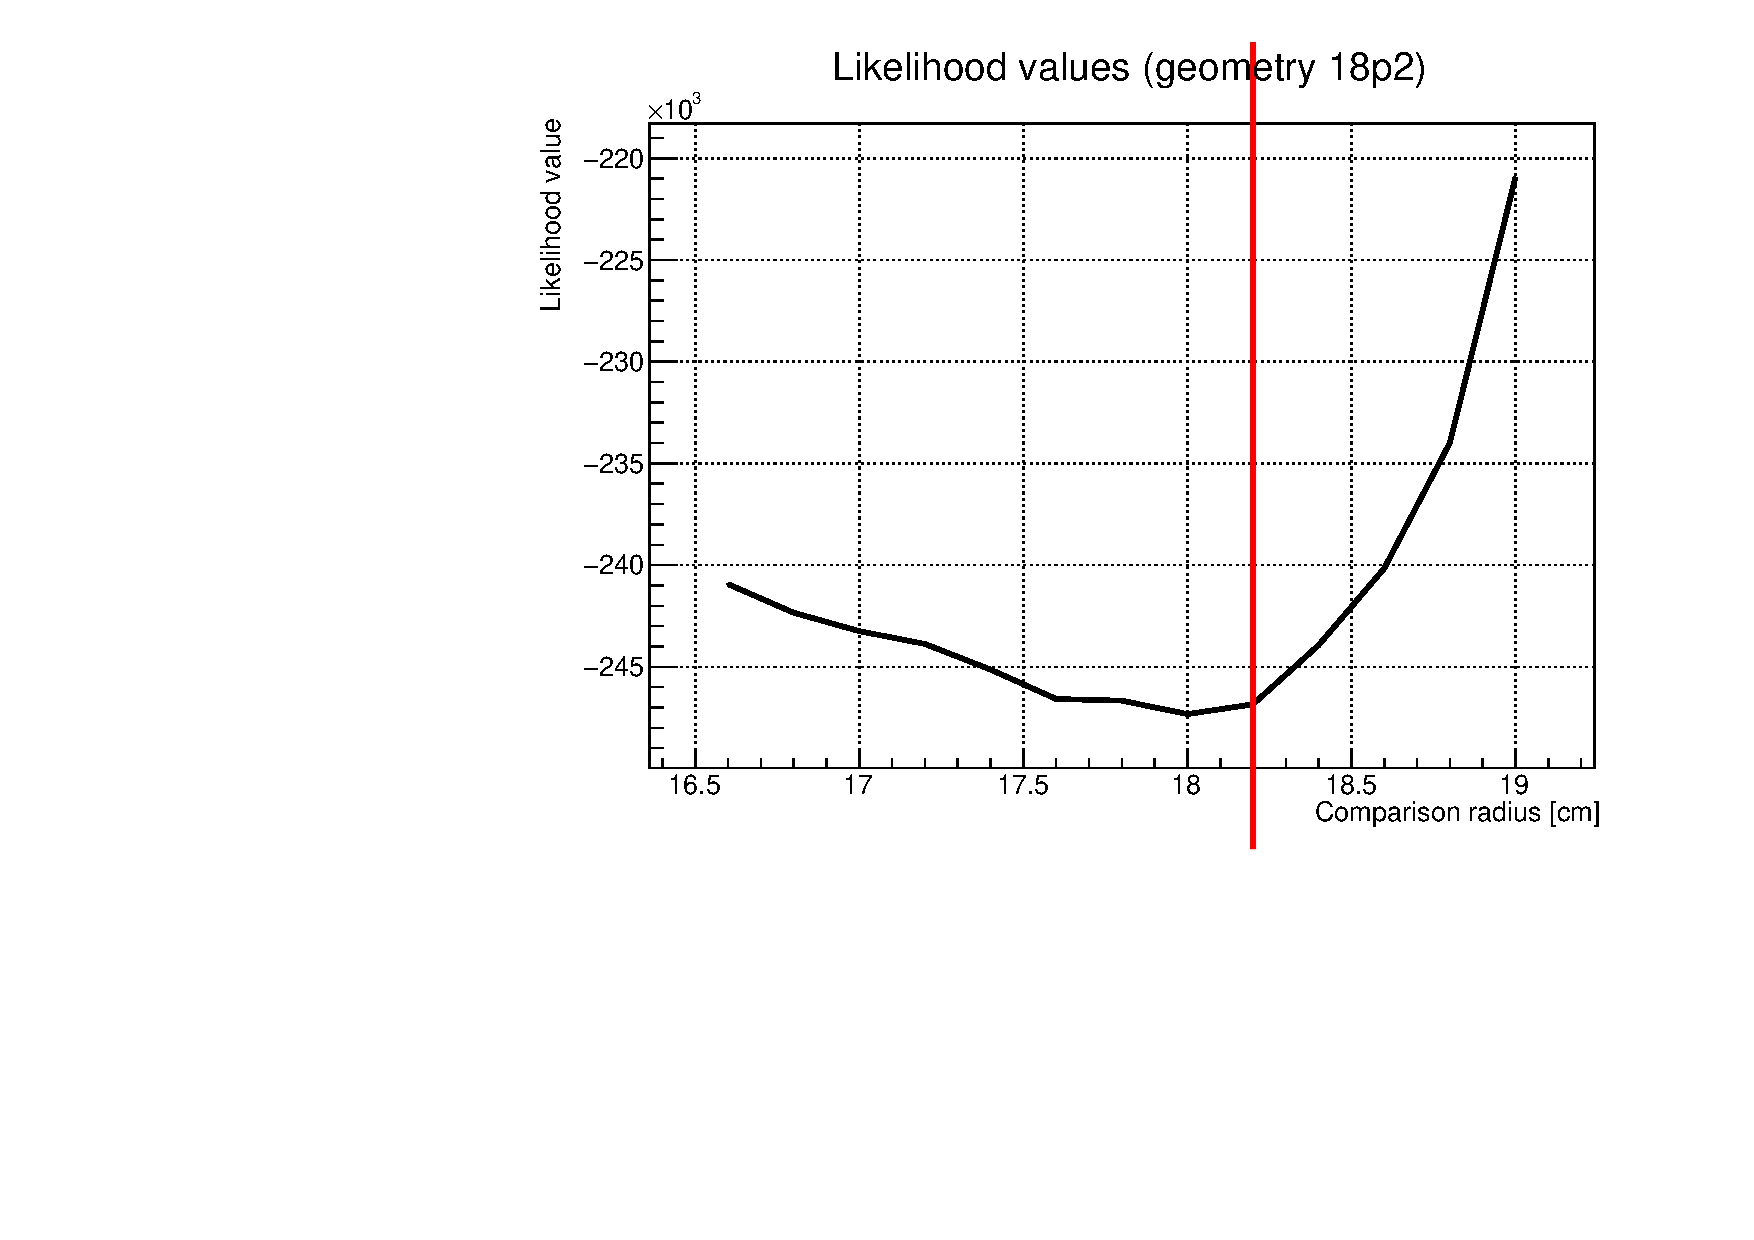
\includegraphics[width=6cm, height=4.6cm]{figs/likelihood100LowStat/likelihood18p2.pdf}
\end{minipage} \hfill
\begin{minipage}[b]{.32\textwidth}
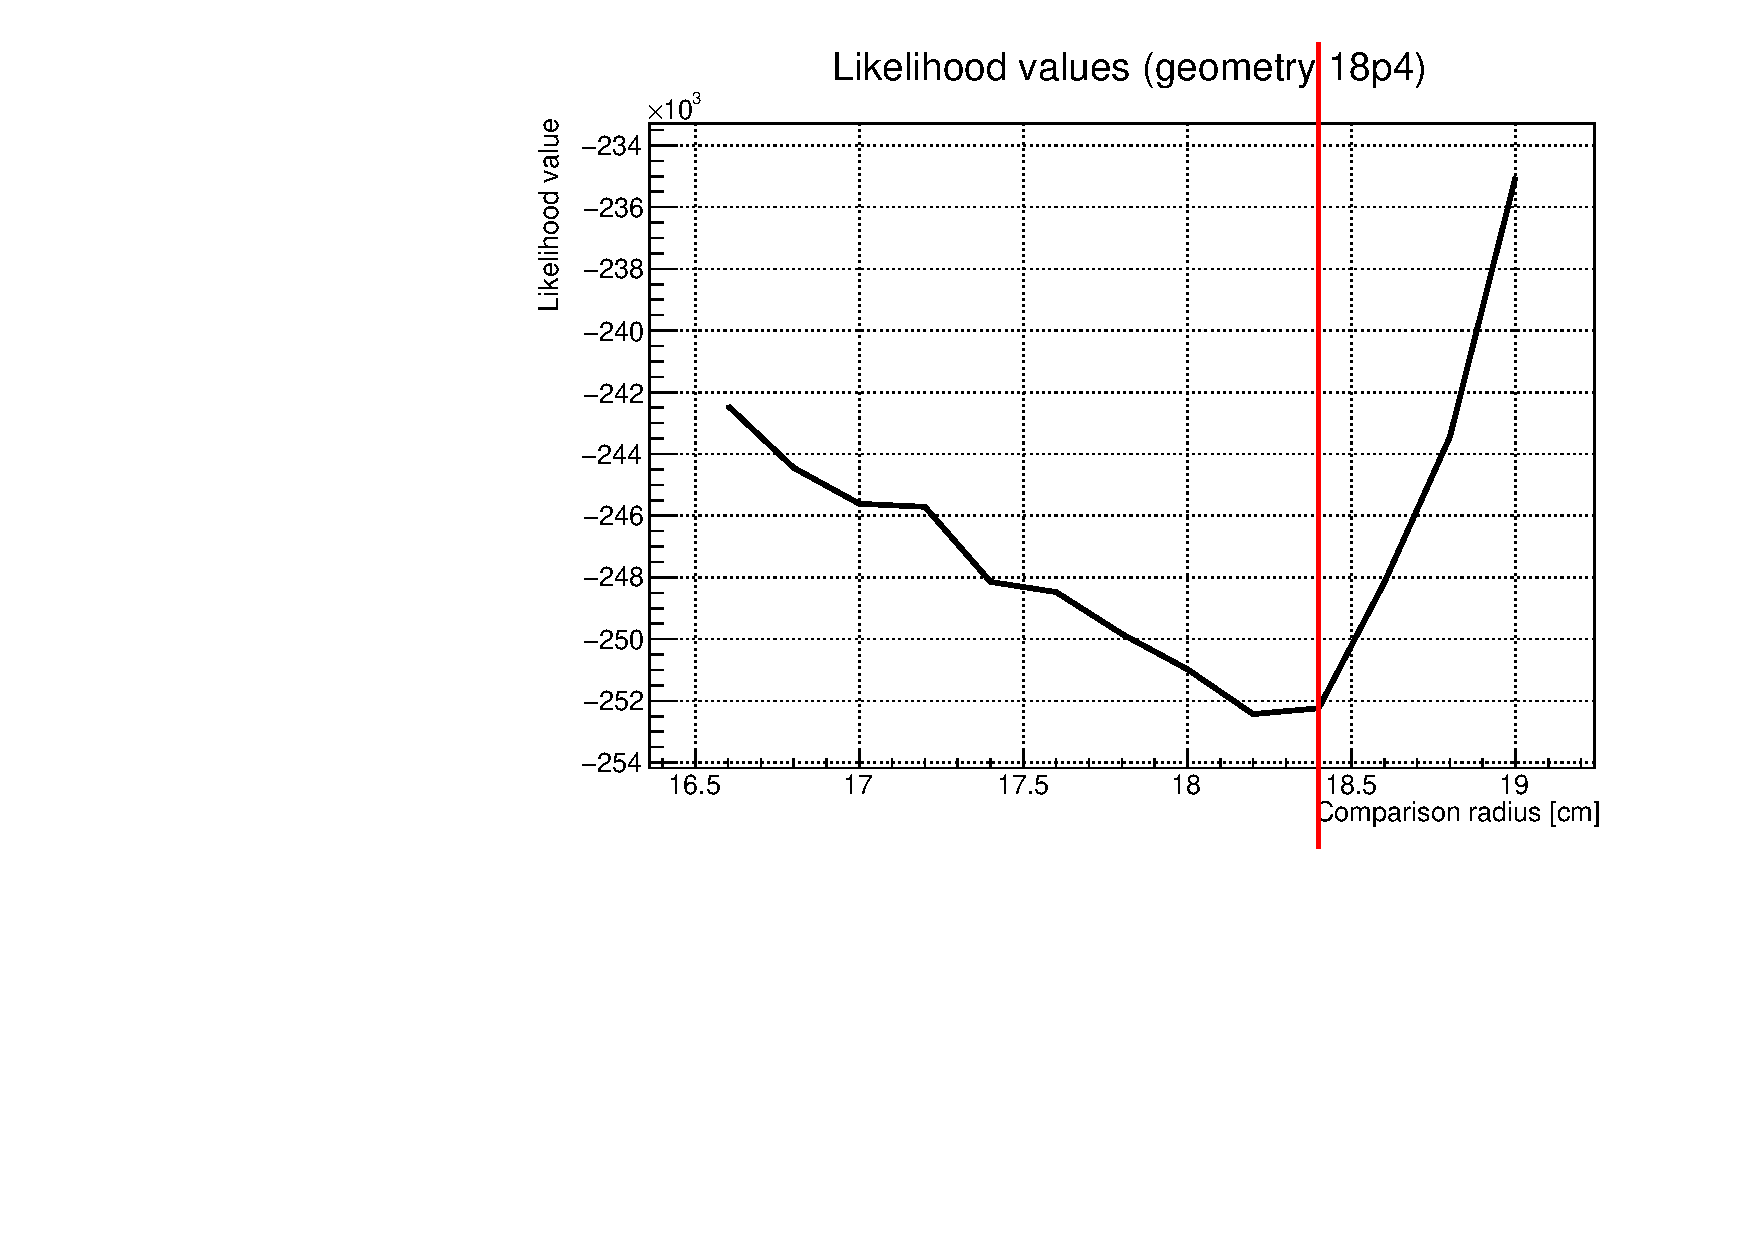
\includegraphics[width=6cm, height=4.6cm]{figs/likelihood100LowStat/likelihood18p4.pdf}
\end{minipage} \hfill \vspace{10pt}

\begin{minipage}[b]{.32\textwidth}
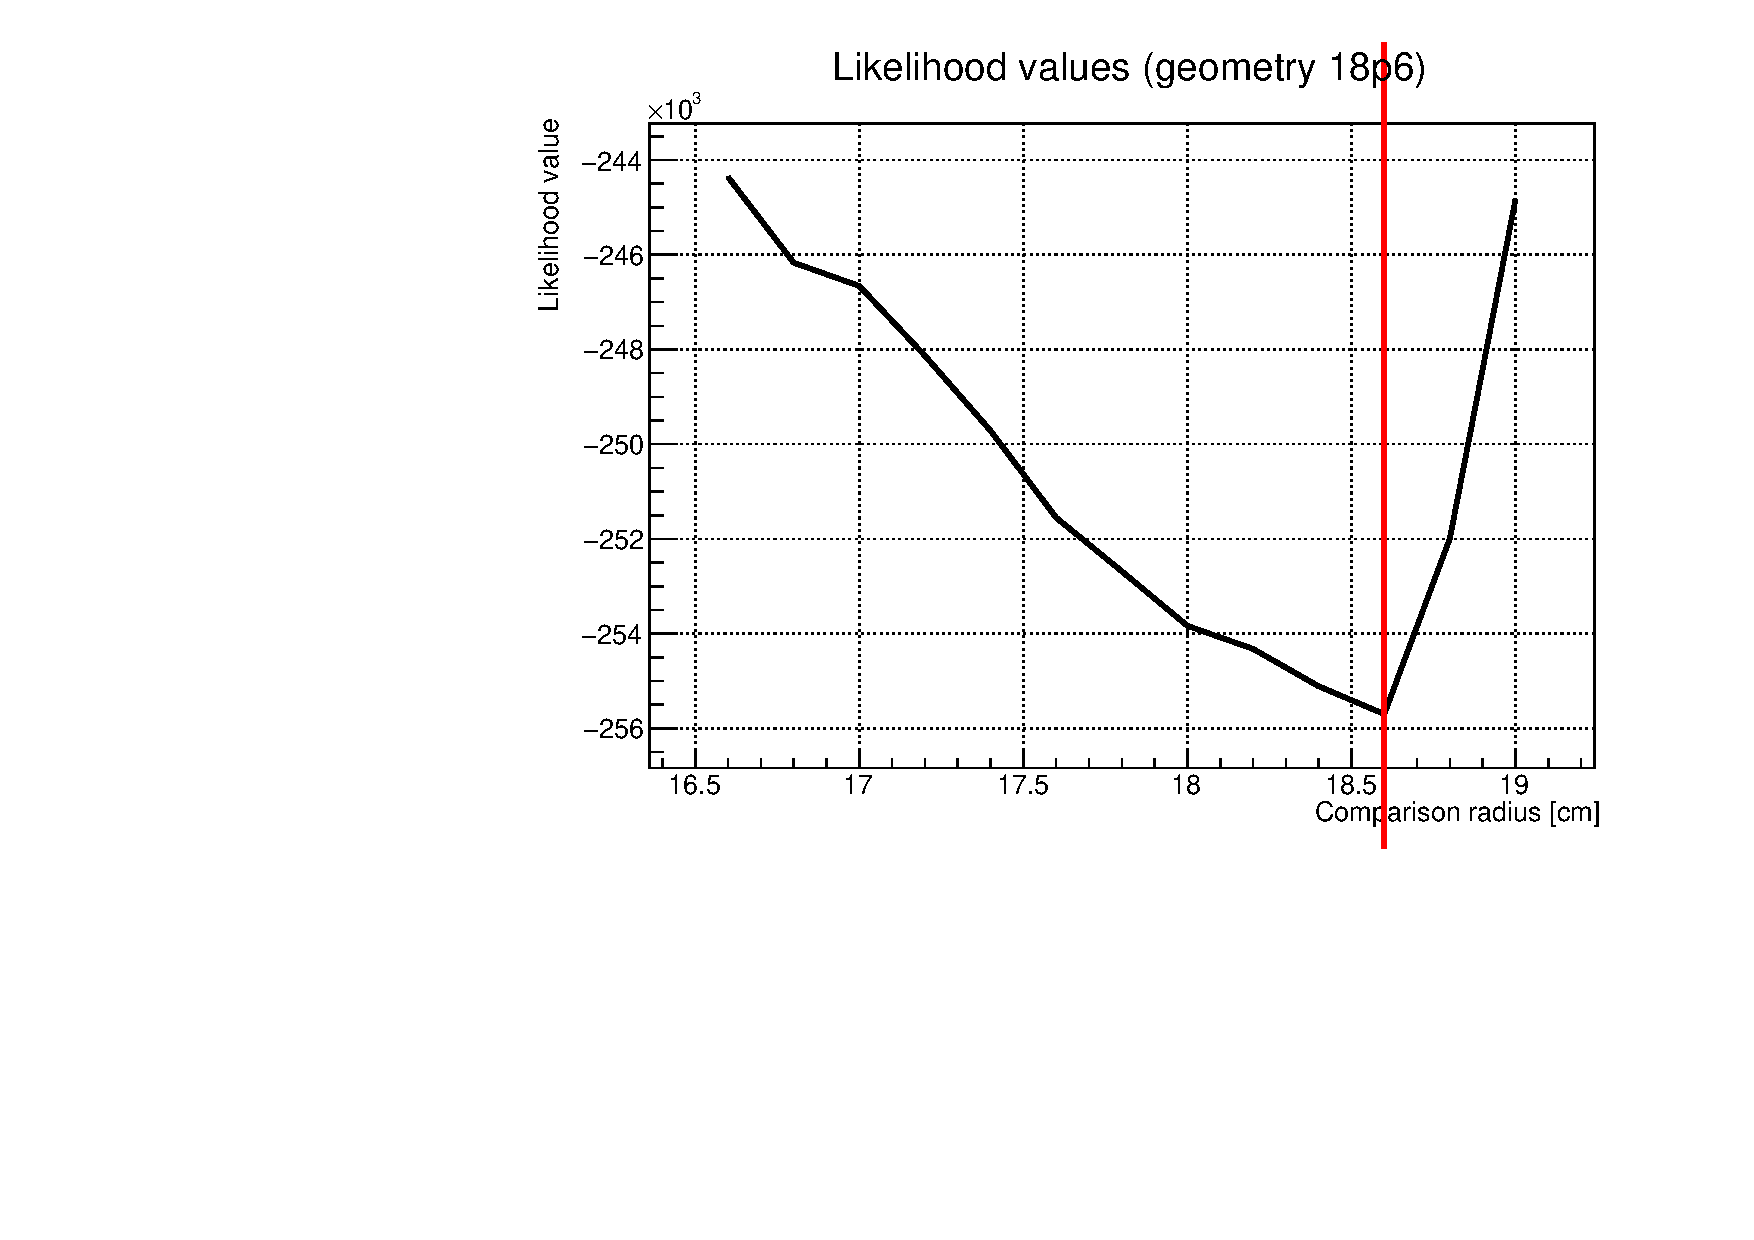
\includegraphics[width=6cm, height=4.6cm]{figs/likelihood100LowStat/likelihood18p6.pdf}
\end{minipage}\hfill
\begin{minipage}[b]{.32\textwidth}
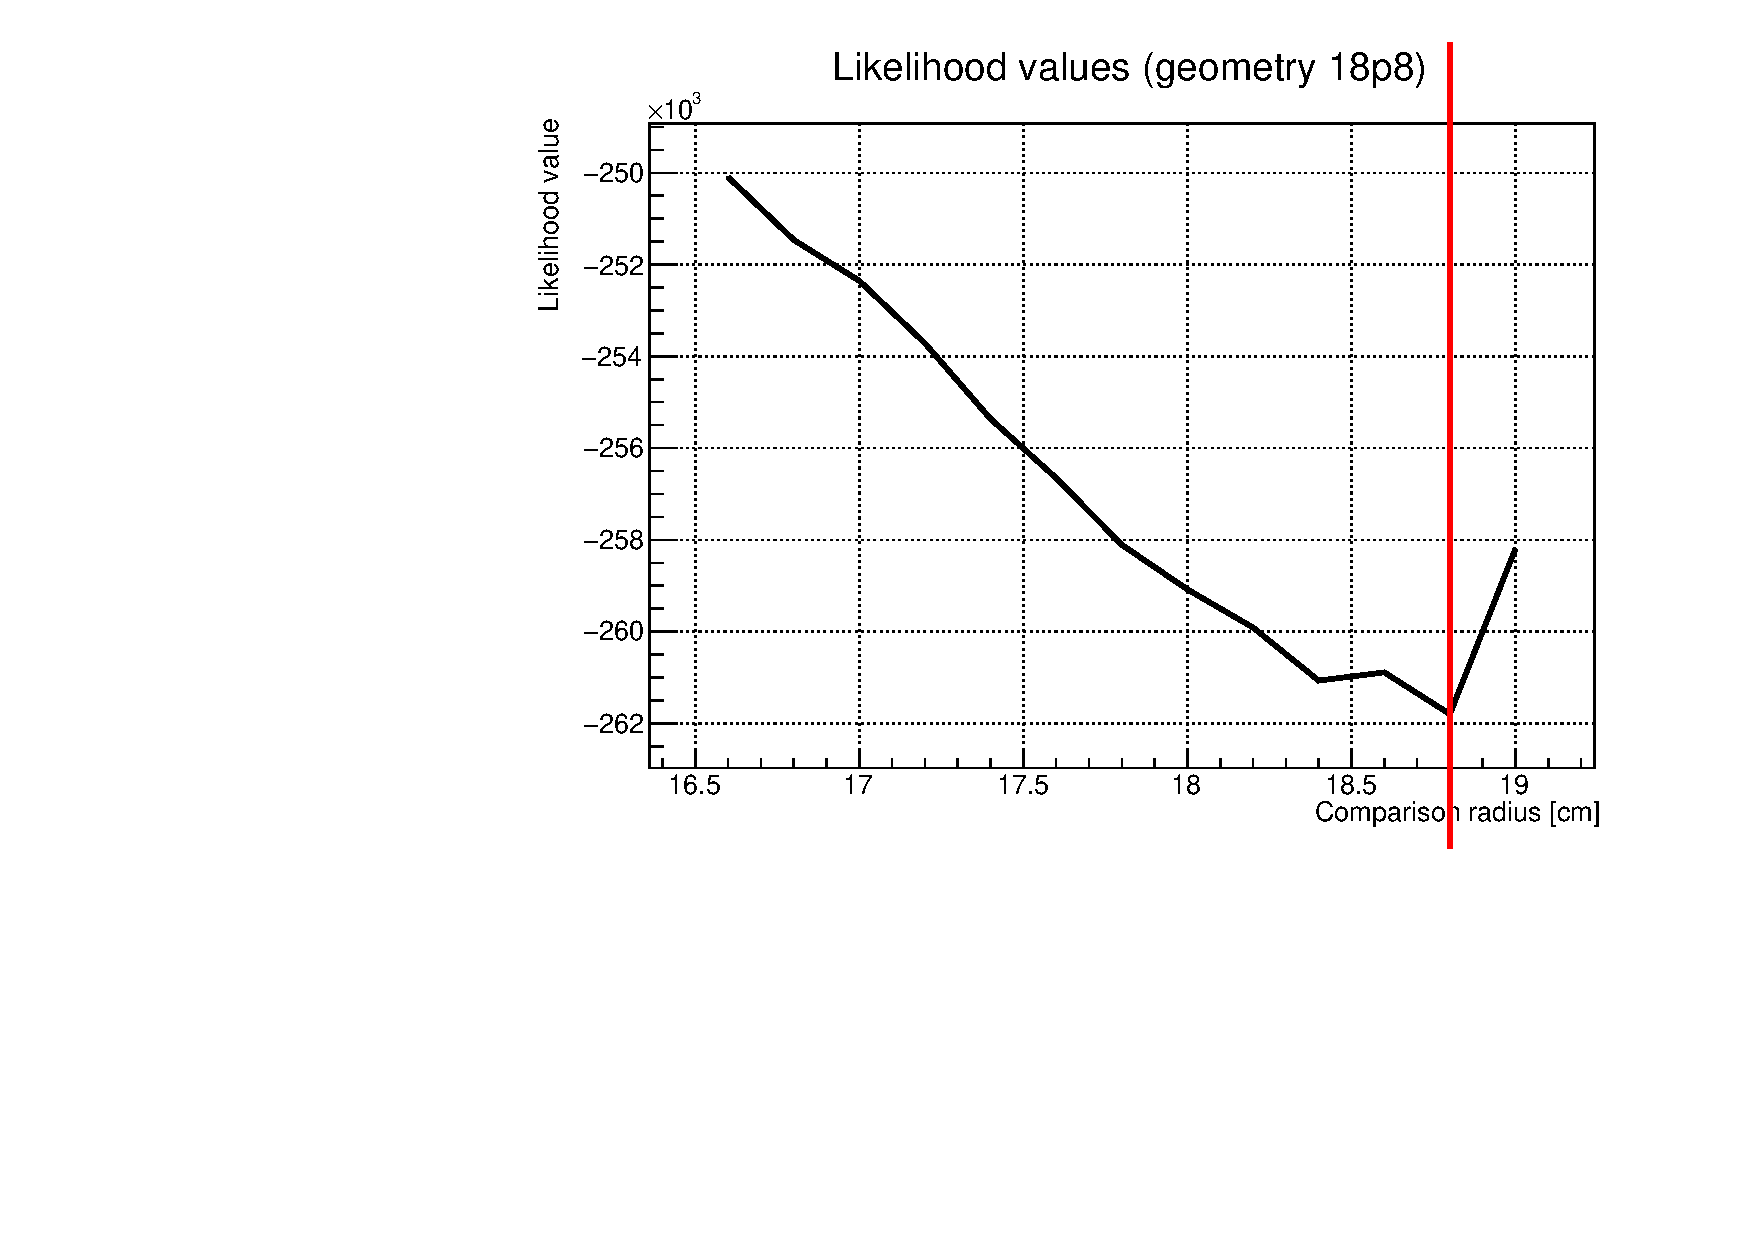
\includegraphics[width=6cm, height=4.6cm]{figs/likelihood100LowStat/likelihood18p8.pdf}
\end{minipage} \hfill
\begin{minipage}[b]{.32\textwidth}
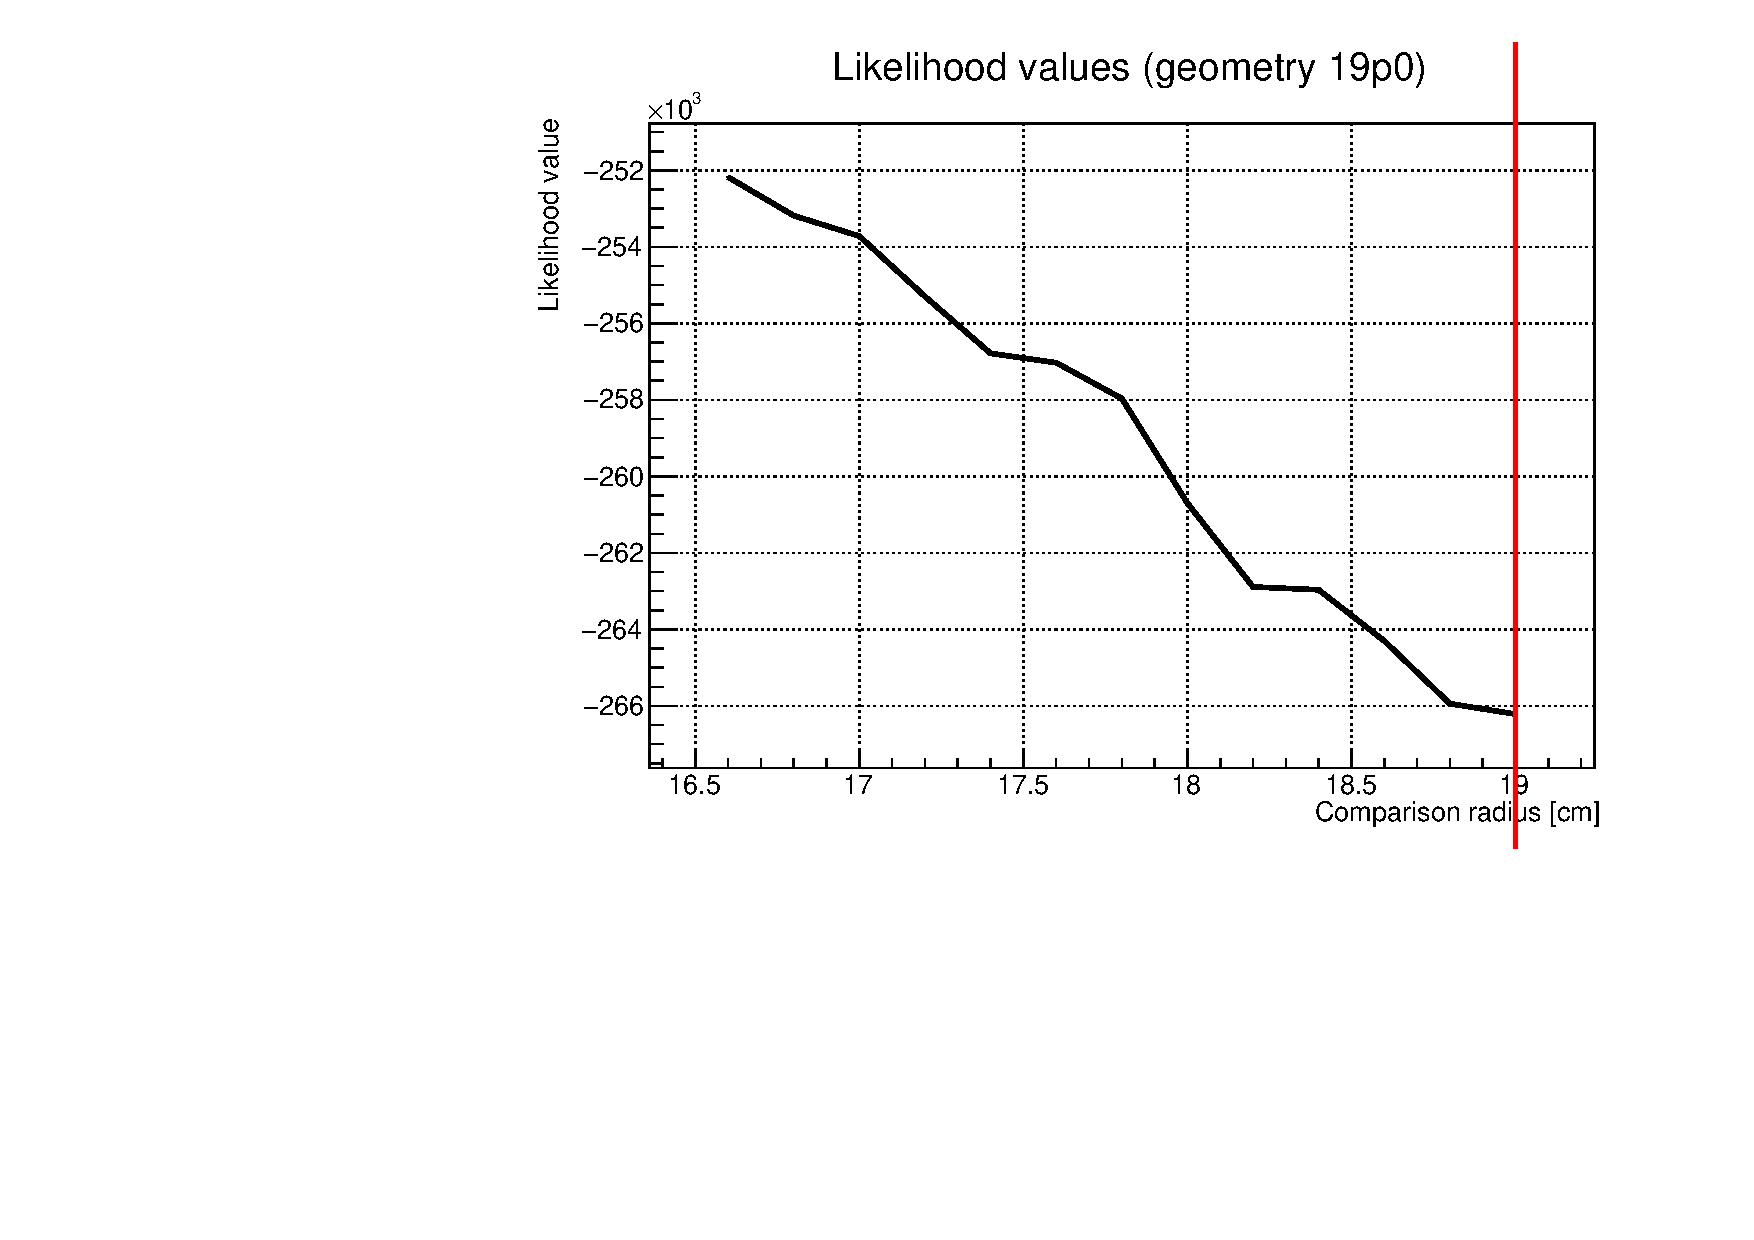
\includegraphics[width=6cm, height=4.6cm]{figs/likelihood100LowStat/likelihood19p0.pdf}
\end{minipage} \hfill
\caption{Likelihood curves obtained by considering different pipe geometries, ranging from 16.8 (on the top left) to 19.0cm of inner radius (on the bottom right), obtained for 100 iterations and 10.000 simulated Monte-Carlo events.}
\label{fig:likelihoods}
\end{figure}

\begin{figure}[htbp]
\centering
\begin{minipage}[b]{.32\textwidth}
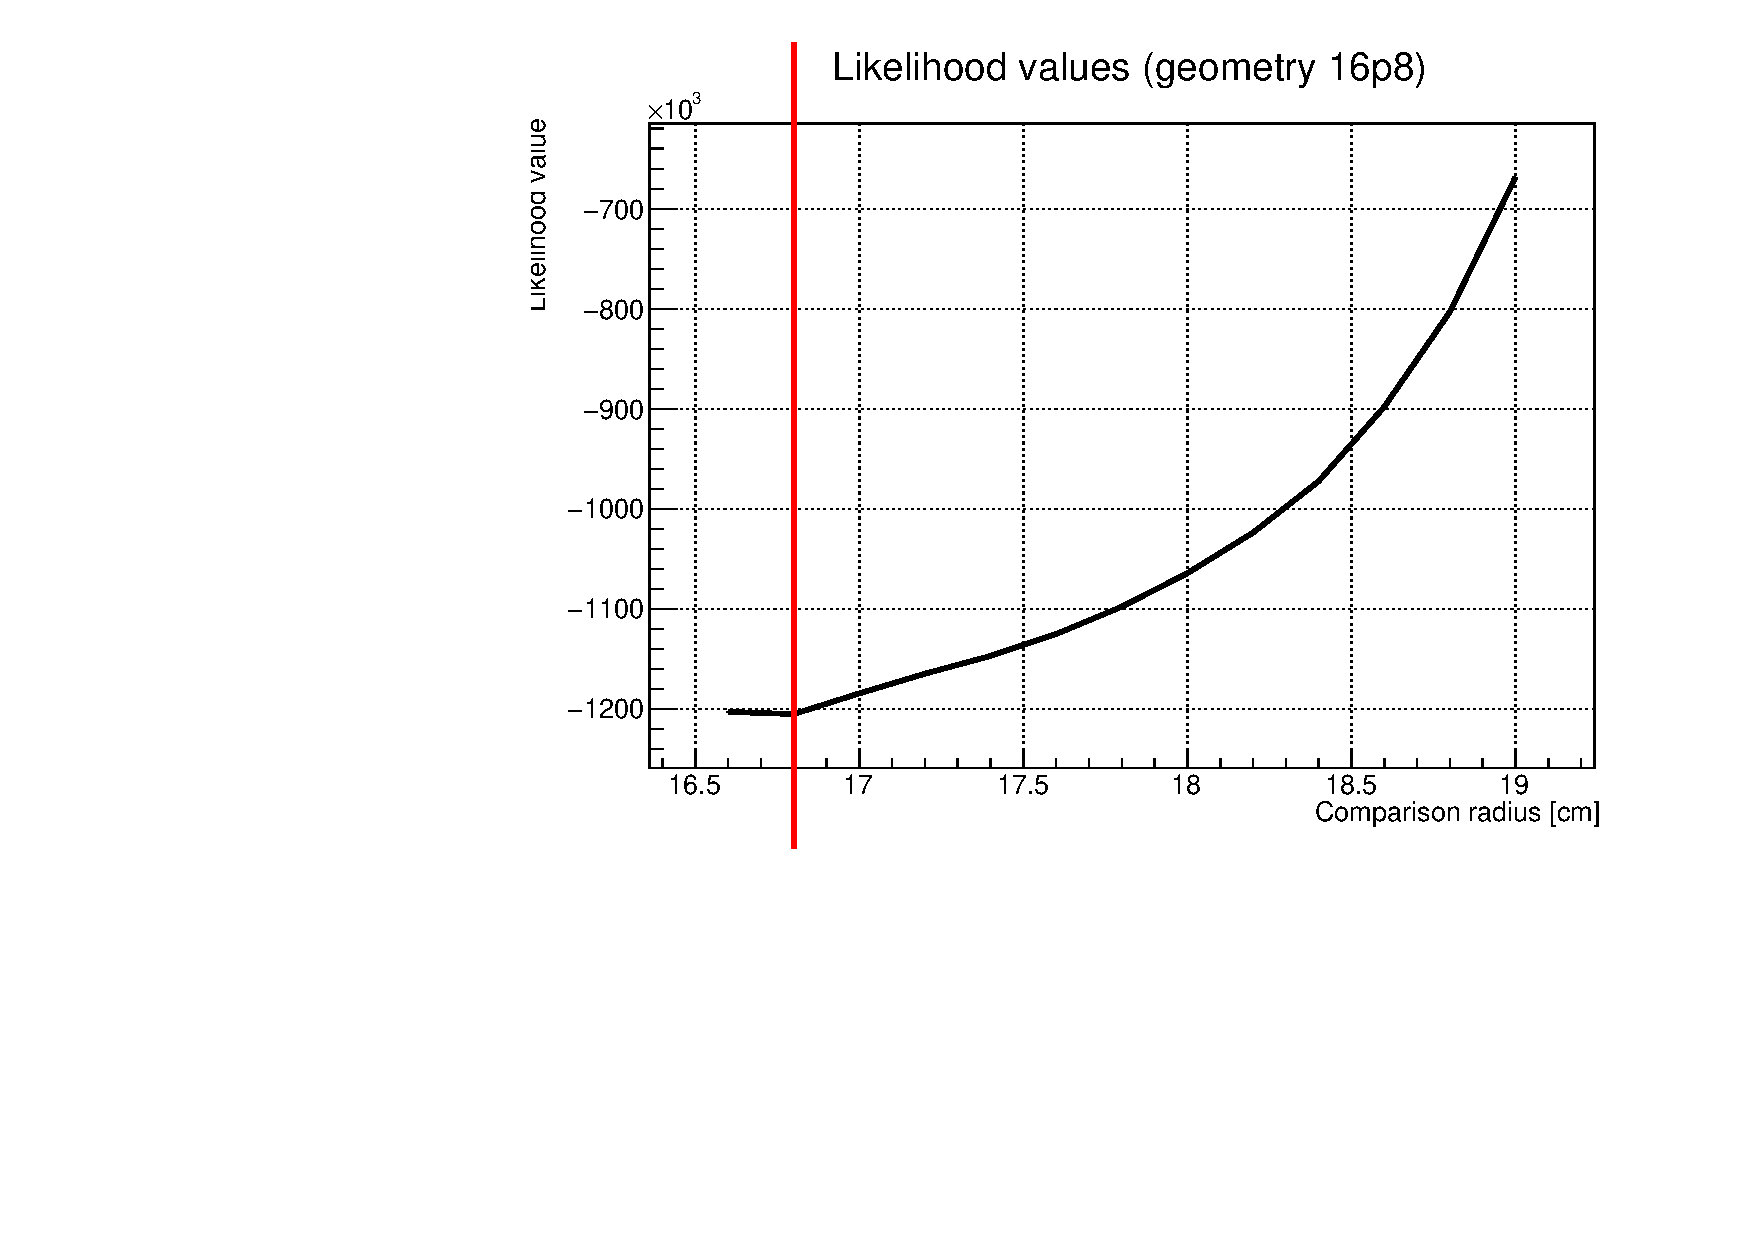
\includegraphics[width=6cm, height=4.6cm]{figs/likelihood100HighStat/likelihood16p8.pdf}
\end{minipage}\hfill
\begin{minipage}[b]{.32\textwidth}
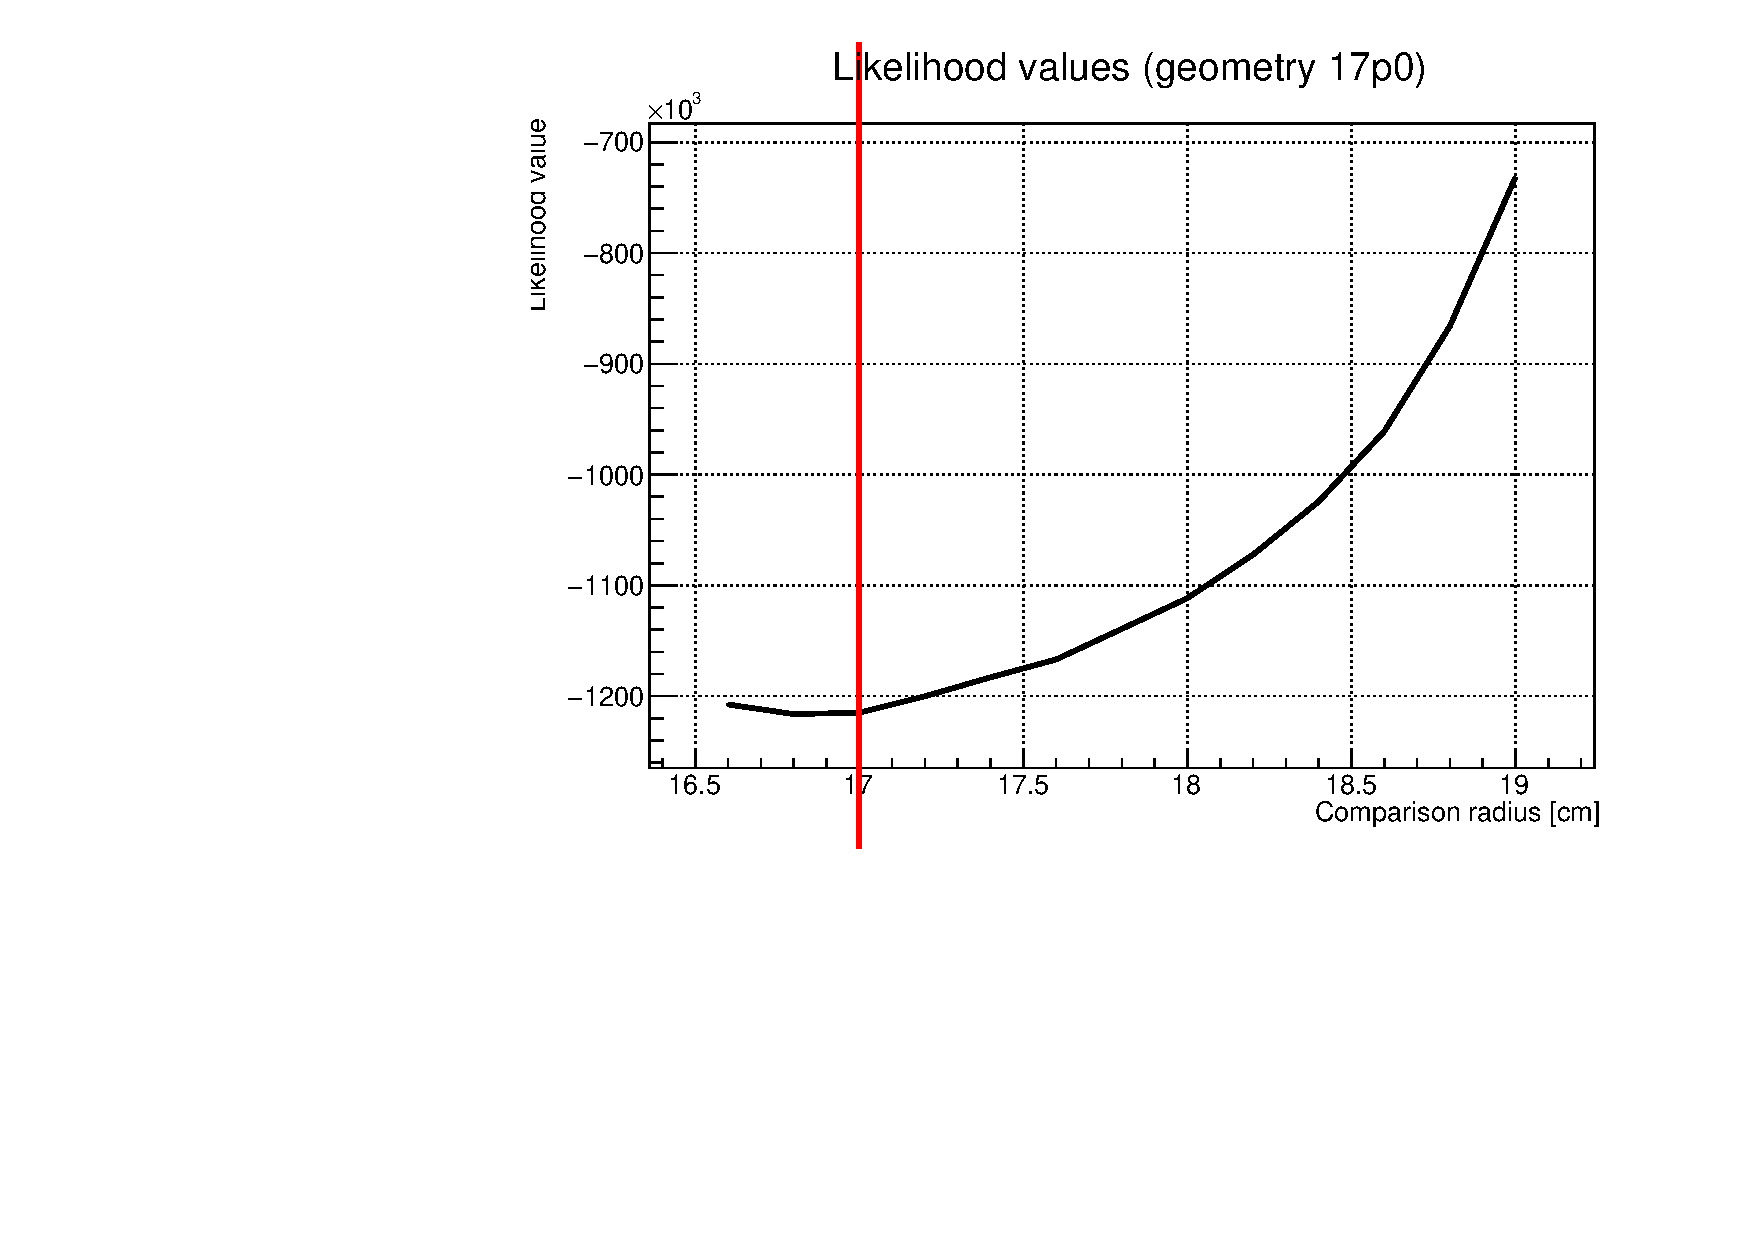
\includegraphics[width=6cm, height=4.6cm]{figs/likelihood100HighStat/likelihood17p0.pdf}
\end{minipage} \hfill
\begin{minipage}[b]{.32\textwidth}
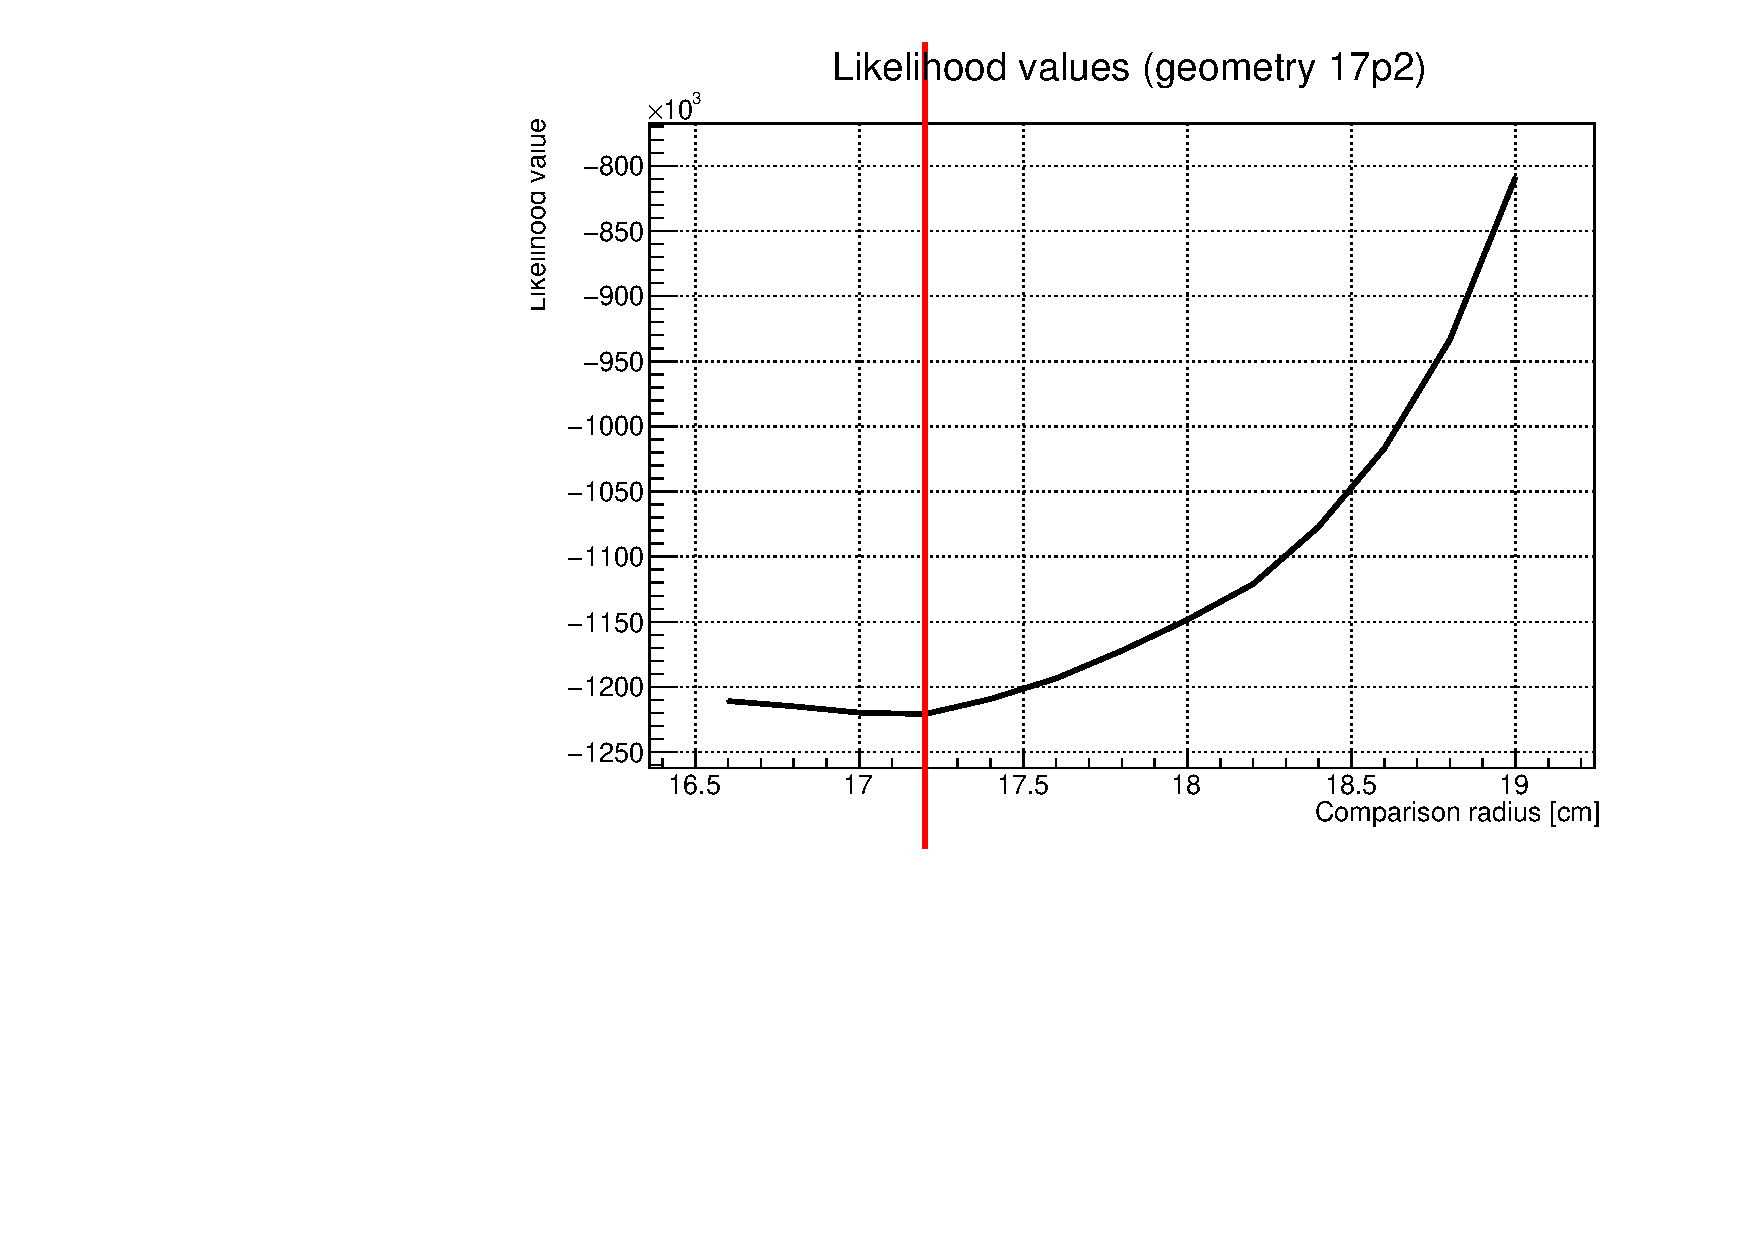
\includegraphics[width=6cm, height=4.6cm]{figs/likelihood100HighStat/likelihood17p2.pdf}
\end{minipage} \hfill \vspace{10pt}

\begin{minipage}[b]{.32\textwidth}
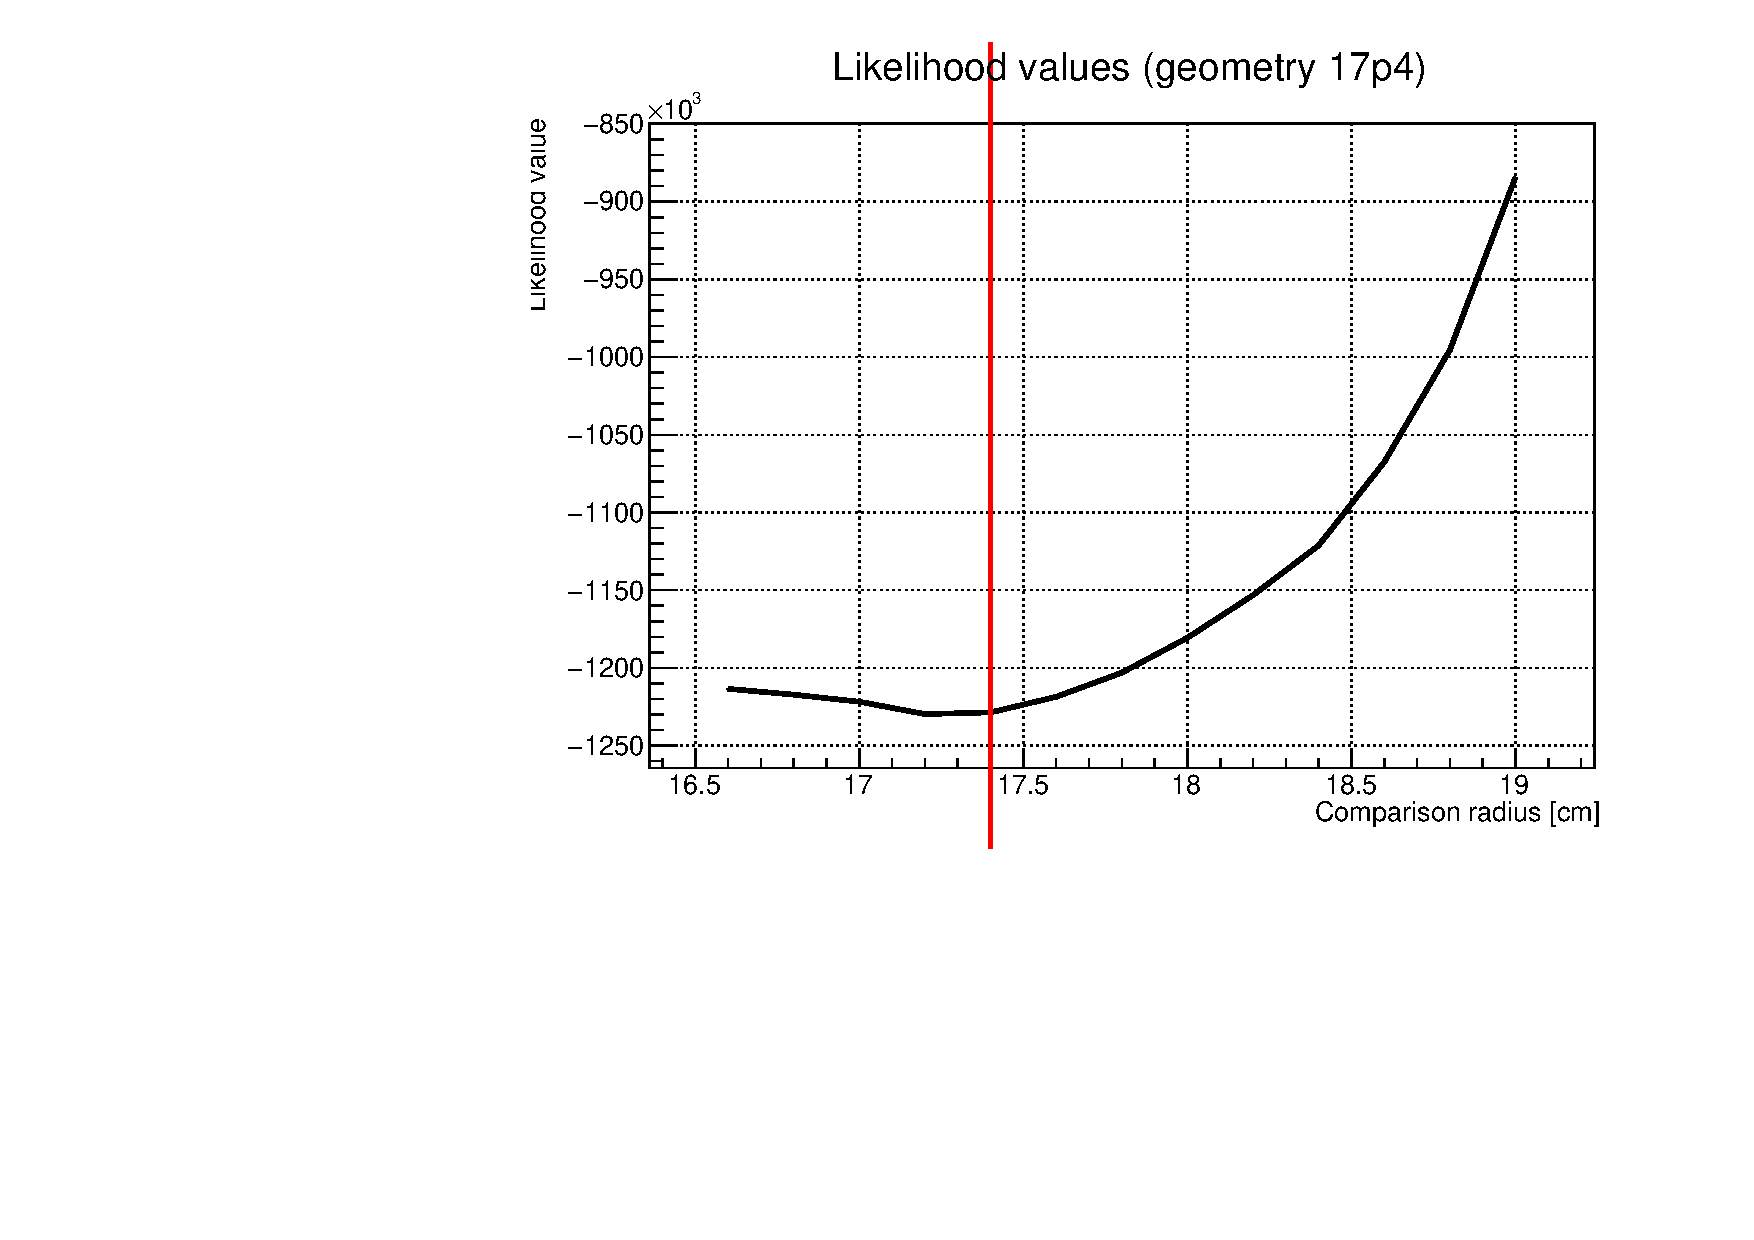
\includegraphics[width=6cm, height=4.6cm]{figs/likelihood100HighStat/likelihood17p4.pdf}
\end{minipage}\hfill
\begin{minipage}[b]{.32\textwidth}
\includegraphics[width=6cm, height=4.6cm]{figs/likelihood100HighStat/likelihood17p6.pdf}
\end{minipage} \hfill
\begin{minipage}[b]{.32\textwidth}
\includegraphics[width=6cm, height=4.6cm]{figs/likelihood100HighStat/likelihood17p8.pdf}
\end{minipage} \hfill \vspace{10pt}

\begin{minipage}[b]{.32\textwidth}
\includegraphics[width=6cm, height=4.6cm]{figs/likelihood100HighStat/likelihood18p0.pdf}
\end{minipage}\hfill
\begin{minipage}[b]{.32\textwidth}
\includegraphics[width=6cm, height=4.6cm]{figs/likelihood100HighStat/likelihood18p2.pdf}
\end{minipage} \hfill
\begin{minipage}[b]{.32\textwidth}
\includegraphics[width=6cm, height=4.6cm]{figs/likelihood100HighStat/likelihood18p4.pdf}
\end{minipage} \hfill \vspace{10pt}

\begin{minipage}[b]{.32\textwidth}
\includegraphics[width=6cm, height=4.6cm]{figs/likelihood100HighStat/likelihood18p6.pdf}
\end{minipage}\hfill
\begin{minipage}[b]{.32\textwidth}
\includegraphics[width=6cm, height=4.6cm]{figs/likelihood100HighStat/likelihood18p8.pdf}
\end{minipage} \hfill
\begin{minipage}[b]{.32\textwidth}
\includegraphics[width=6cm, height=4.6cm]{figs/likelihood100HighStat/likelihood19p0.pdf}
\end{minipage} \hfill
\caption{Likelihood curves obtained by considering different pipe geometries, ranging from 16.8 (on the top left) to 19.0cm of inner radius (on the bottom right), obtained for 100 iterations and 50.000 simulated Monte-Carlo events.}
\label{fig:likelihoods2}
\end{figure}

\begin{figure}[htbp]
\centering
\begin{minipage}[b]{.32\textwidth}
\includegraphics[width=6cm, height=4.6cm]{figs/likelihood250LowStat/likelihood16p8.pdf}
\end{minipage}\hfill
\begin{minipage}[b]{.32\textwidth}
\includegraphics[width=6cm, height=4.6cm]{figs/likelihood250LowStat/likelihood17p0.pdf}
\end{minipage} \hfill
\begin{minipage}[b]{.32\textwidth}
\includegraphics[width=6cm, height=4.6cm]{figs/likelihood250LowStat/likelihood17p2.pdf}
\end{minipage} \hfill \vspace{10pt}

\begin{minipage}[b]{.32\textwidth}
\includegraphics[width=6cm, height=4.6cm]{figs/likelihood250LowStat/likelihood17p4.pdf}
\end{minipage}\hfill
\begin{minipage}[b]{.32\textwidth}
\includegraphics[width=6cm, height=4.6cm]{figs/likelihood250LowStat/likelihood17p6.pdf}
\end{minipage} \hfill
\begin{minipage}[b]{.32\textwidth}
\includegraphics[width=6cm, height=4.6cm]{figs/likelihood250LowStat/likelihood17p8.pdf}
\end{minipage} \hfill \vspace{10pt}

\begin{minipage}[b]{.32\textwidth}
\includegraphics[width=6cm, height=4.6cm]{figs/likelihood250LowStat/likelihood18p0.pdf}
\end{minipage}\hfill
\begin{minipage}[b]{.32\textwidth}
\includegraphics[width=6cm, height=4.6cm]{figs/likelihood250LowStat/likelihood18p2.pdf}
\end{minipage} \hfill
\begin{minipage}[b]{.32\textwidth}
\includegraphics[width=6cm, height=4.6cm]{figs/likelihood250LowStat/likelihood18p4.pdf}
\end{minipage} \hfill \vspace{10pt}

\begin{minipage}[b]{.32\textwidth}
\includegraphics[width=6cm, height=4.6cm]{figs/likelihood250LowStat/likelihood18p6.pdf}
\end{minipage}\hfill
\begin{minipage}[b]{.32\textwidth}
\includegraphics[width=6cm, height=4.6cm]{figs/likelihood250LowStat/likelihood18p8.pdf}
\end{minipage} \hfill
\begin{minipage}[b]{.32\textwidth}
\includegraphics[width=6cm, height=4.6cm]{figs/likelihood250LowStat/likelihood19p0.pdf}
\end{minipage} \hfill
\caption{Likelihood curves obtained by considering different pipe geometries, ranging from 16.8 (on the top left) to 19.0cm of inner radius (on the bottom right), obtained for 250 computations iterations and 10.000 simulated Monte-Carlo events.}
\label{fig:likelihoods3}
\end{figure}

As we can see in these results, the minimum of the likelihood curve is almost always exactly at the place where we expected it to be. This means that with this algorithm, we do manage to reach in most of the cases a precision at least equal to the order of the step chosen, currently set to 2 millimeters. It also seems that increasing the number of simulated events from 10.000 to 50.000 is interesting, as it decreases the small fluctuations observed in the first case, resulting in a smoother curve, even though it also multiplies by a factor 5 the computing time, moving from 20 minutes to produce a single top to more than an hour. On the other hand, moving the number of iterations from 100 to 250 does not seem to have much of an impact.

In any case, these last results show that by using the algorithm developed here, we are capable of determining the actual inner width of a pipe using cosmic muon and without destructing this pipe, the initial objective of this work, with a precision of the order of 1 millimeter for the experimental conditions considered, therefore solving the initial problem set.























\chapter{Conclusions}

In conclusion, this work was designed with one simple objective in mind: using the detectors already built by the company Muon Systems and the muon tomography technique in order to determine the inner properties of a general geometry (considered for this work to be a steel pipe made out of two cylinders, even though the code has been developed to be able to simply add more complex geometries in the future), using several statistical concepts and a general Maximum Likelihood Estimate method to analyze the results obtained. This allowed us to determine the thickness of different pipes using data science and a natural source of energy, without having to destroy the pipes, which is an extremely interesting process that can be useful and applied to many different industries.

The principle of this statistical approach presented here is quite simple: in order to study the inner properties of a steel pipe, we can put a detector above the pipe, measuring the initial position and directions of cosmic muons, and another detector below the volume considered, to compute the actual deviation suffered by the cosmic muons when crossing the gap between the two detectors. Since this deviation in position and angle is expected to be larger when crossing the steel pipe than the air, given the difference in density of these two medium, we expected to be able to estimate the actual width of the pipe crossed from such measurements of the positional and angular deviations. 

Additionally, we defined in the process a brand new Generator in the process, allowing us to generate Monte-Carlo simulations of such cosmic muons and to propagate them across our geometry using the Moli\`ere's theory of multiple scattering. This is interesting in the sense that it allows to remove the dependance on Geatn4, highly realiable but quite slow. This way of generating Monte-Carlo experiments has been thoroughly check within this work. 

At the end of the day, by implementing advanced statistical methods to solve this problem, we managed to estimate the actual width of such steel pipes with a precision of the order of 1 millimeter, therefore solving the problem which was originally presented.

\section{Suggested improvements}

Of course, this work is only a first approach to this particular problem, and many different improvements could be added in the future in order to improve and/or generalize the results obtained:

\begin{itemize}
    \item First of all, as previously stated, this work was focused on a typical approach related to steel pipes typically used in the industry in general. The framework is ready to include additional and more exotic geometries to study them as well, even though this has not been done in this particular work. Even pipes could be quite easily studied in greater details using this framework, by for example considering additional parameters to characterize them, such as a possible dependence of the width of the pipe with respect to the position. Being able to find weak spots in particular locations in the pipe itself would be something of great value for the industry.
    \item Another interesting idea might be to consider ionization as well, therefore performing an absorption muography experiment. In this work, we did not consider the loss of energy suffered by a muon when crossing the volume studied since it is expected to be quite low, but such information could help us increase the precision of the measurements performed.
    \item In this work, we did not consider detector effects even though by interacting with the incident cosmic muons, they have an effect on them, even though this effect is supposed to be quite small. Simulating in a precise way this interaction could also improve the precision of the method.
    \item Another limiting factor is the limited spatial resolution of the detector used, with wires placed every 4 millimeters. Finding techniques to build a detector with an improved spatial resolution is obviously expected to give better results.
    \item A detailed study of the errors associated to the method presented here has not been performed but will be useful for the industry as well.
    \item Finally, our results have been quite limited because of the computing power which was available. Given the fact that the determination of the likelihood required us to do complex and long calculations, with loops of tens of thousands of elements within each other, we had to limit as much as possible several parameters, such as the number of iterations performed to compute the likelihood. Increasing this parameter is expected to give better results, but also increase the computing time. Running this code on more powerful and/or distributed machines is therefore also expected to give better results.
\end{itemize}

%\begin{appendices}
  
%\chapter{Appendix1}
  
%\end{appendices}

\addcontentsline{toc}{chapter}{Bibliography}

\begin{thebibliography}{1}

\bibitem{SM}
\href{https://arxiv.org/abs/hep-ph/0510281}{G. Altarelli,
"The Standard Model of Particle Physics",
CERN-PH-TH/2005-206, 2005}

\bibitem{topQuark} 
\href{https://arxiv.org/abs/hep-ex/9503003}{D0 Collaboration,
"Observation of the Top Quark",
Phys.Rev.Lett.74:2632-2637, 1995}

\bibitem{tauNeutrino} 
\href{https://arxiv.org/abs/hep-ex/0012035}{DONUT Collaboration, 
"Observation of Tau Neutrino Interactions",
Phys.Lett.B504:218-224, 2001}

\bibitem{HiggsDiscovery1} 
\href{https://arxiv.org/abs/1207.7235}{S. Chatrchyan et al.,
"Observation of a new boson at a mass of 125 GeV with the CMS experiment at the LHC",
Phys.Lett.B716:30-61, 2012 [arXiv: 1207.7235]
}

\bibitem{HiggsDiscovery2} 
\href{https://arxiv.org/abs/1207.7214}{G. Aad et al.,
"Observation of a new particle in the search for the Standard Model Higgs boson with the ATLAS detector at the LHC", 
Phys.Lett.B716:1-29, 2012 [arXiv: 1207.7214]}

\bibitem{SMFermions}
\href{https://link.springer.com/chapter/10.1007/978-3-030-24370-8_2#citeas}{S. Manzoni, 
"The Standard Model and the Higgs Boson",
Physics with Photons Using the ATLAS Run 2 Data, Springer Theses, 2019
}

\bibitem{PDGMuons}
\href{http://pdg.lbl.gov/2018/listings/rpp2018-list-muon.pdf}{
"Muon", Particle Data Group, 2018}

\bibitem{cosmicPDG}
\href{http://pdg.lbl.gov/2017/reviews/rpp2017-rev-cosmic-rays.pdf}{
"Cosmic rays", Particle Data Group, 2017}

\bibitem{muonDiscovery}
\href{http://web.ihep.su/dbserv/compas/src/neddermeyer37/eng.pdf}{S.H. Neddermeyer and C.D. Anderson,
"Note on the Nature of Cosmic-Ray Particles", 
Physical Review Vol. 51, 1936}

\bibitem{PDGScat}
\href{http://pdg.lbl.gov/2019/reviews/rpp2019-rev-passage-particles-matter.pdf}{
"Passage of Particles Through Matter", Particle Data Group, 2019}

\bibitem{Moliere}
\href{https://journals.aps.org/pr/abstract/10.1103/PhysRev.89.1256}{H.A. Bethe,
"Moli\`ere's Theory of Multiple Scattering", 
Physical Review Vol. 89, 1953}

\bibitem{Egypt}
\href{https://ui.adsabs.harvard.edu/abs/1970Sci...167..832A/abstract}{L. Alvarez et all.,
"Search for Hidden Chambers in the Pyramid", 
Science, vol. 167 (3919), 1970}

\bibitem{waste}
\href{https://ieeexplore.ieee.org/document/8069918}{L. Frazao et all.,
"High-resolution imaging of nuclear waste containers with muon scattering tomography", 
2016 IEEE Nuclear Science Symposium}

\bibitem{lava}
\href{https://ui.adsabs.harvard.edu/abs/1970Sci...167..832A/abstract}{J. Marteau et all.,
"Muons tomography applied to geosciences and volcanology", 
Nuclear Instruments and Methods in Physics Research Section A: Accelerators, Spectrometers, Detectors and Associated Equipment vol.695 pp23-28, 2012
}

\bibitem{CRY}
\href{https://arxiv.org/pdf/0811.0187.pdf}{M. Holmann et all, "GEANT4 Simulation of a Cosmic Ray Muon Tomography System with Micro-Pattern Gas Detectors for the Detection of High-Z Materials" [arXiv:0811.0187]}

\bibitem{Geant4}
\href{https://www.sciencedirect.com/science/article/pii/S0168900203013688}{S. Agostinelli et all, "Geant4: a simulation toolkit", Nuclear Instruments and Methods in Physics Research Section A, vol. 506 (3), pages 250-303}

\bibitem{PDF}
\href{https://www.math24.net/probability-density-function/}{Math24, "Probability Density Function", as seen in May 2020}

\bibitem{bandwidth}
\href{https://www.hindawi.com/journals/jps/2015/242683/}{S. Chen, "Optimal Bandwidth Selection for Kernel Density Functionals Estimation", Journal of Probability and Statitics vol. 2015 (242683), as seen in June 2020}

\bibitem{scikit}
\href{https://scikit-learn.org/stable/auto_examples/neighbors/plot_kde_1d.html}{Scikit-learn: Machine Learning in {P}ython, "Simple 1D Kernel Density Estimation", as seen in July 2020}

\end{thebibliography}

\end{document}
